\documentclass[11pt]{gsasthesis} % 10,11 and 12pt fonts allowed

%%%%%%%%%%%%%%%% PACKAGES YOU PROBABLY WANT %%%%%%%%%%%%%%%%
% Include packages you want. The gsasthesis style file already includes
% packages "setspace" and "tocbibind".

\usepackage{etex} % extend the number of registers

% GSAS: "all margins should be at least 1 inch."
\usepackage[margin={1.2in}]{geometry}
% If you want asymmetric margins for two-sided documents, use the "twoside"
% option, as in
% \usepackage[top=1in,bottom=1.5in,left=1in,right=1.5in,twoside]{geometry} The
% left and right options become inner and outer margins The default horizontal
% latex margin ratio is 2:3. The default vertical top:bottom margin ratio is 2:3
% also. You can also set it directly by passing the hmarginratio option to the
% geometry package, as in
% \usepackage[top=1in,left=1in,vmarginratio=2:3,hmarginratio=2:5,twoside]{geometry}

% Appendix package. Not necessary, but it does make managing appendices easier
\usepackage[titletoc]{appendix}

%%%%%%%%%%%%%%%% PACKAGES MAY WANT %%%%%%%%%%%%%%%%

% sideways tables and figures
\usepackage{rotating}

% tables that spill over multiple pages
\usepackage{longtable}

% references
\usepackage{natbib}

\usepackage{comment}

\usepackage{multirow, booktabs}
\usepackage{amsmath}
\usepackage{amssymb}
\usepackage{amsfonts}
\usepackage{makecell}

\usepackage{enumitem}

\usepackage{graphicx}
\usepackage{soul}
\usepackage[normalem]{ulem}
\usepackage{subcaption}

\newcolumntype{L}[1]{>{\raggedright\let\newline\\\arraybackslash\hspace{0pt}}m{#1}}
\newcolumntype{C}[1]{>{\raggedright\let\newline\\\arraybackslash\hspace{0pt}}m{#1}}

\usepackage{CJKutf8}
\usepackage{pifont}
\newcommand{\xmark}{\ding{55}}

\usepackage{rotating}
\usepackage{pdflscape}

% fonts that are nicer than defaults
\usepackage[sc]{mathpazo}
%\usepackage{courier}
\usepackage[mono=false]{libertine}  % I personally favour this font

% Use 8-bit encoding that has 256 glyphs, pretty please
\usepackage[utf8]{inputenc}
\usepackage[T1]{fontenc}

% babel is required for blindtext, which generates random text
\usepackage[english]{babel}
\usepackage{blindtext}

% math support
\usepackage{amsmath}

% Slightly tweak font spacing for aesthetics
\usepackage{microtype}



% You need the footmisc package with the stable option if you want to have
% footnotes inside section titles, for example to say that a particular chapter
% has been co-authored with someone. The multiple option ensures that there is a
% comma between two consecutive footnotes
\usepackage[stable,multiple]{footmisc}


% Nicer captions
\RequirePackage[font=small,format=plain,labelfont=bf,textfont=it]{caption}
\addtolength{\abovecaptionskip}{1ex}
\addtolength{\belowcaptionskip}{1ex}

% Add a period to the end of an abbreviation unless there's one
% already, then \xspace.
\makeatletter
\DeclareRobustCommand\onedot{\futurelet\@let@token\@onedot}
\def\@onedot{\ifx\@let@token.\else.\null\fi\xspace}

\def\eg{\emph{e.g}\onedot} \def\Eg{\emph{E.g}\onedot}
\def\ie{\emph{i.e}\onedot} \def\Ie{\emph{I.e}\onedot}
\def\cf{\emph{cf}\onedot} \def\Cf{\emph{Cf}\onedot}
\def\etc{\emph{etc}\onedot} \def\vs{\emph{vs}\onedot}
\def\wrt{w.r.t\onedot} \def\dof{d.o.f\onedot}
\def\iid{i.i.d\onedot} \def\wolog{w.l.o.g\onedot}
\def\etal{\emph{et al}\onedot}
\makeatother

\usepackage{nicefrac}
\usepackage[table,dvipsnames]{xcolor}
\usepackage{subcaption}
\usepackage{physics}
\usepackage{algorithm}
\usepackage{algorithmic}
\usepackage{bm}


%%%%%%%%%%%%%%%% COMPULSORY FIELDS %%%%%%%%%%%%%%%%

\title{Learning Depth and Motion from Visual Geometry: Unifying Stereo, Semantic, and Temporal Information} % needs to match title on DAC
\author{GUAN, Tongfan} % full name as it appears on your GSAS record, needs
                          % to match name on DAC
\degreename{Doctor of Philosophy}
\degreefield{Mechanical and Automation Engineering} % Official name of subject as listed in GSAS
                                % handbook
\department{Mechanical and Automation Engineering} % official name of department
\degreemonth{March} % Month of Defense (i.e. month when DAC was signed)
\degreeyear{2026} % Year the DAC was signed
\principaladvisor{Professor AA}

% Optionally, you can add a second advisor, but you can't have three
%\secondadvisor{Professor George Secondary}



\begin{document}

%%%%%%%%%%%%%%%% FRONTMATTER %%%%%%%%%%%%%%%%

\pagenumbering{roman} % GSAS wants roman page numbers for frontmatter

% the following four pages are required in that order. The first two pages are
% not allowed to have page numbers, this is taken care of in the class file.
\thesistitlepage
%\copyrightpage
\committeepage
\begin{abstract}
Recovering accurate 3D structure and camera motion from visual observations is a foundational challenge in computer vision and embodied robotics.
This capability underpins a wide range of applications,  from autonomous navigation and robotic manipulation to augmented reality.
Yet, depth and motion are not directly observable from images and must instead be inferred from underlying geometric relationships.
In natural visual perception, multiple sources of geometric information are available, including stereo correspondences across viewpoints, semantic and structural context from monocular observations, and temporal dynamics induced by motion over time.
While each source provides complementary strengths, effectively unifying these heterogeneous representations within a unified learning framework remains an open challenge.

This thesis investigates how neural networks can learn visual geometry from stereo, semantic, and temporal information to enable robust depth and motion perception.
We begin by mastering the first cue, \ie, explicit stereo correspondence, through a neural Markov Random Field formulation for stereo matching.
This approach embeds structured correspondence reasoning directly into the learning process and establishes a principled foundation for correspondence-based depth estimation.
Building on this foundation, we address the challenge of incorporating semantic context. 
We propose a cross-modal framework that bidirectionally aligns monocular and stereo representations within a shared latent geometric space.
This alignment facilitates knowledge transfer between distinct depth cues and highlights the critical role of semantic understanding in resolving geometric ambiguity.
These insights naturally motivate a transition from explicit correspondence modeling toward more holistic and unified representations.

To this end, we develop a unified architecture based on a single-stream Vision Transformer that directly regresses depth from visual inputs, whether a stereo pair or a single image.
This model demonstrates that geometric principles can be implicitly captured through global reasoning, without the need for explicit cost-volume construction or carefully engineered matching pipelines.
Finally, we extend this unified philosophy to the temporal domain to tackle the inherent coupling of camera ego-motion and scene geometry in monocular video. 
Moving beyond conventional visual representations, we propose a geometry-native Transformer that operates directly on estimated optical flow fields and monocular depth priors.
At its core lies a novel Transformer block that decouples global rigid motion from local structural parallax, steering the network toward a physically consistent geometric consensus while suppressing interference from dynamic objects.
Through joint reasoning over temporal motion fields and monocular depth priors, the proposed approach seamlessly resolves degenerate kinematic configurations, such as pure camera rotation or nearly forward translation, that typically challenge classic optimization methods like bundle adjustment.
The result is a framework that accurately and simultaneously recovers camera pose and scene geometry, even under severe kinematic degeneracies and in complex dynamic environments.

Together, these contributions establish a unified perspective on learning from visual geometry. By systematically integrating stereo correspondence, semantic context, and temporal dynamics, this thesis demonstrates that robust depth and motion perception can be achieved through a coherent framework that leverages complementary geometric structure across space, modality, and time.
In doing so, it advances the development of geometry-centric visual perception systems toward greater robustness, generality, and physical fidelity.
\end{abstract}

\begin{cabstract}


\end{cabstract}

% Center headings for table of contents, LOT, and LOF and make them smaller so
% that "Abstract", "Acknowledgments" and "Contents" all look alike. Comment out
% if you want the default. If you want more control, use the "tocloft" package.
\renewcommand{\contentsname}{\protect\centering\protect\Large Contents}
\renewcommand{\listtablename}{\protect\centering\protect\Large List of Tables}
\renewcommand{\listfigurename}{\protect\centering\protect\Large List of Figures}

\tableofcontents % Table of contents

% The rest of the front matter: Lists of tables, figures, dedication and
% acknowledment is optional. Comment out whatever you don't like
\listoftables
\listoffigures
\begin{acknowledgments}
  Acknowledgement here.   
  
  %I would like to thank my thesis committee members for their valuable and constructive comments. Furthermore, I want to express my gratitude to the professors in the Department of Systems Engineering and Engineering Management.  
\end{acknowledgments}
%\begin{dedication}
%  To my parents and my girl friend. 
%\end{dedication}


%%%%%%%%%%%%%%%% MAIN BODY %%%%%%%%%%%%%%%%
\pagenumbering{arabic} % reset page numbering and switch to arabic

% Introductory chapter. Comment out if you don't have an intro chapter, but I
% think most committees expect you to have one.
% Don't number the intro chapter, but add to to the table of contents
%\addcontentsline{toc}{chapter}{Introduction}
\chapter{Introduction}\label{ch:intro}
\section{Background}
The ability to perceive the three-dimensional (3D) structure of the surrounding world and one's own movement within it is a cornerstone of visual intelligence.
For biological organisms, this capability is essential to survival, enabling navigation through space, manipulation of objects, and interaction with dynamic environments.
For artificial systems, it is equally critical: robots must localize and map their surroundings to navigate autonomously; augmented reality devices must register virtual content with the physical world; and autonomous vehicles must perceive pedestrians, obstacles, and road geometry to operate safely.
Despite the diversity of these applications, they converge on a common computational problem: recovering structure and motion from sensor observations.
Among available sensing modalities, vision is particularly attractive due to its low cost, high resolution, and passive nature, making it applicable across a broad spectrum of real-world scenarios.

Yet, this problem is fundamentally challenging due to the limited observability of three-dimensional structure in images.
Images are two-dimensional (2D) projections of the 3D world.
During this projection, the depth dimension is collapsed and motion becomes entangled with scene structure.
As a result, the pixels themselves contain no direct measurement of how far a surface lies or how the camera is moving.
A single point in an image could correspond to a nearby object or a distant one; a moving pixel could result from camera motion, object motion, or both.
The physical world must instead be inferred from \textbf{visual geometry}, which is the set of geometric relationships that govern the interaction between scene structure, camera motion, and image formation.
Although revealed through multiple complementary sources of information, these relationships are implicit, often ambiguous, and frequently corrupted by noise, occlusion, and dynamic elements in real-world environments.
Stereo correspondence, given calibrated cameras, admits a unique geometric solution in principle, yet remains challenging in practice due to textureless regions, occlusions, and reflective surfaces.
Monocular depth, by contrast, is fundamentally ill-posed: a single image provides no direct geometric constraints, requiring the injection of learned priors to resolve uncertainty.
Temporal motion introduces its own complexities, intertwining camera ego-motion with scene structure in ways that must be disentangled.
The central question of this thesis is therefore: How can we design neural architectures that reliably recover depth and motion by reasoning about the geometric structure inherent in visual data, despite the distinct challenges posed by each observational setting?

The human visual system offers important insight into this problem.
It seamlessly integrates multiple complementary sources of geometric information, adaptively weighting different cues depending on their reliability and availability in a given context~\cite{ban2012integration}.
Such integration is thought to arise from shared internal representations that unify diverse sensory signals, including binocular disparity and motion parallax, into a coherent percept of the three-dimensional world.
Neuroimaging evidence showed that visual area V3B/KO exhibited more discriminative responses when both cues concurrently signaled depth than when either cue was presented alone.
Moreover, information provided by one cue alone was diagnostic of depth indicated by the other, suggesting a shared neural representation that transcends cue-specific coding~\cite{ban2012integration}.
These findings point to a cortical architecture that favors cue fusion over independent processing streams, providing a biological inspiration for addressing the challenges of robust depth and motion estimation through unified geometric representations.

In contrast, despite substantial progress in recent years, existing computational approaches to depth and motion estimation remain largely fragmented across different observational settings.
Stereo matching~\cite{scharstein2002taxonomy,hirschmuller2005accurate}, monocular depth estimation~\cite{eigen2014depth,Ranftl2022}, and structure-from-motion~\cite{schoenberger2016sfm,pan2024glomap} have typically been studied in isolation, each relying on distinct intermediate representations that limit their ability to transfer knowledge across modalities or to generalize under challenging conditions.
Methods are tailored to specific observational settings rather than unified by a common representational framework.
As a result, they often struggle in scenarios where individual cues are weak, ambiguous, or conflicting.
This separation motivates a closer review of how existing methods represent and combine visual evidence across stereo, monocular, hybrid, and temporal settings.
The following section therefore first examines the prior art along these lines before returning to the contributions of this thesis.

\noindent\textbf{Spatial Geometry (Stereo Correspondence).} When a scene is observed from two distinct viewpoints simultaneously, the relative displacement, or disparity, of corresponding points provides a direct geometric signal for depth.
In a standard rectified binocular setup, where images are aligned such that corresponding points lie on the same horizontal line, the relationship between disparity $d$ and depth $z$ is given by $z=f\cdot b / d$, where $f$ is the focal length and $b$ is the baseline distance between the two cameras~\cite{hartley2003multiple}.
This simple triangulation makes stereo correspondence a well-posed route to depth, grounded in explicit geometric principles.
However, the practical difficulty lies in establishing reliable correspondences.
The cue fails in textureless regions where matching is ambiguous, at occlusions where points are visible in only one view, and under specularities where appearance varies with viewpoint.
Stereo correspondence therefore provides a geometrically precise but brittle starting point, motivating the integration of additional cues.

\noindent\textbf{Cognitive Geometry (Semantic Context).} A single image does not provide explicit correspondence, yet humans are able to infer depth from it with remarkable accuracy.
This capability arises from internalized prior knowledge about the structure of the world: objects such as cars exhibit characteristic physical scales, the sky is typically distant, and road surfaces provide strong perspective cues as they recede.
Such semantic and structural context, learned from experience, offers powerful constraints for resolving geometric ambiguities in scenarios where correspondence-based cues are weak or unreliable.
Integrating this cognitive geometry with explicit spatial geometry is therefore essential for achieving robust depth perception.

\noindent\textbf{Temporal Geometry (Motion and Structure).} While binocular and monocular static images provide powerful depth cues, the most general and ubiquitous source of visual geometry is temporal motion.
When a camera moves through the world, the resulting image sequence provides geometric constraints through motion parallax, whereby nearby objects exhibit larger apparent motion than distant ones.
This temporal signal inherently couples camera ego-motion with scene structure, offering rich observations from which both can be recovered simultaneously.
However, this coupling also introduces fundamental challenges: separating motion induced by the camera from that arising from independently moving objects is inherently ambiguous, and certain camera motion patterns, such as pure rotation or forward translation, lead to degenerate geometric configurations.
Effective reasoning over temporal information therefore requires models that can disentangle these factors while maintaining consistency with the underlying geometric structure.
As the most general and ubiquitous source of visual geometry, temporal motion forms a critical foundation for unified depth and motion perception.

Together, stereo correspondence, semantic context, and temporal motion define the three complementary pillars of visual geometry that inform this thesis.
These complementary sources of geometric information form the conceptual foundation of this thesis.
Yet, existing computational approaches largely treat these pillars in isolation, fragmenting the representation of geometry across disparate pipelines rather than exploiting their synergies.
This separation leaves significant room for more integrated geometric representation learning.

\noindent\textbf{Relevance to Robotics.} In robotic systems, visual geometry provides the foundation for state estimation and action: metric depth supports localization, mapping, navigation, and obstacle avoidance, while semantic structure helps robots interpret and interact with their surroundings.
The contributions of this thesis address successive requirements of this perception stack.
NMRF improves structured stereo correspondence; structure-aware depth completion enhances the reliability of geometric supervision; BridgeDepth combines monocular semantic priors with stereo constraints; DispViT learns a shared geometry-semantic representation, and GeNT extends this perspective to temporal depth and motion for streaming local mapping.
The thesis therefore focuses on computer-vision models as the geometric perception layer of robotics, while leaving downstream planning and control outside its scope.

\section{Related Works}

This section reviews existing approaches to depth and motion estimation from visual geometry, organized according to the thesis narrative from spatial correspondence, to monocular semantic priors, to hybrid monocular-stereo reasoning, and finally to temporal motion.
This ordering first establishes the strengths and limits of each source of evidence, then exposes why a progressive move toward shared geometric representation learning is needed.

\subsection{Stereo Matching: Spatial Geometry}

Stereo matching estimates depth from a pair of rectified image by finding correspondences between left and right views.
The fundamental relationship $z=f\cdot b / d$ links disparity $d$ to depth $z$, making stereo a geometrically well-posed problem.
However, the practical challenge lies in establishing reliable correspondences under real-world conditions such as textureless regions, occlusions, specular reflections, and repetitive patterns.

\noindent\textbf{Classical approaches} formulate stereo matching as an energy minimization problem, combining a data term (matching cost) with a smoothness prior.
Early approaches rely on local window-based matching~\cite{scharstein2002taxonomy}, while global methods introduced Markov Random Fields (MRFs)~\cite{szeliski2008comparative} to enforce spatial consistency.
Grounded in principled probabilistic modeling, MRF-based formulation dominated pre-deep-learning stereo methods, as evidenced by their prevalence on benchmarks like Middlebury~\cite{scharstein2002taxonomy}.
Within the MRF framework, stereo matching is cast as a labeling problem: each pixel $o$ receives a disparity label $z_o$, and the set of all labels is $\{z_o\}$. The joint probability over labels and observations ${\mathbf{x}_o}$ takes the form:
\begin{equation}
	p(\{z_o\},\{\mathbf{x}_o\})\propto \prod_o \Phi(z_o,\mathbf{x}_o) \prod_{(o,p)} \Psi(z_o,z_p),
	\label{eq:mrf-tra}
\end{equation}
where $\Phi$ (unary) and $\Psi$ (pairwise) are non‑negative potential functions, and $(o,p)$ indexes neighboring pixel pairs.
Maximum a posteriori (MAP) inference corresponds to minimizing the negative log-likelihood of this distribution.
%Taking the negative logarithm turns Maximum A Posteriori (MAP) inference into an energy minimization problem.
Semi‑Global Matching (SGM)~\cite{hirschmuller2007stereo} remains a popular solver which strikes a favorable trade-off between accuracy and efficiency, approximating 2D smoothness via multiple 1D dynamic programming passes.
While these classical techniques are interpretable and geometrically grounded, they struggle in ill-posed regions where the data term is ambiguous.

 \noindent\textbf{Learning-based stereo matching.} The introduction of convolutional neural network (CNNs) marked a turning point for stereo matching.
 Early work by Žbontar and LeCun~\cite{zbontar2016stereo} replaced hand-engineering feature extraction with learned patch similarities, whereas DispNetC~\cite{mayer2016large} demonstrated the feasibility of end-to-end disparity regression.
 A dominant subsequent paradigm formalizes disparity estimation as 3D cost volume processing: GC-Net~\cite{kendall2017end} pioneered end-to-end learning with 3D convolutions, and PSMNet~\cite{chang2018pyramid} incorporated spatial pyramid pooling to aggregate multi‑scale contextual information.
 Many follow‑up studies~\cite{guo2019group,cheng2019learning,xu2022attention,shen2022pcw} further refined cost volume construction and aggregation, achieving incremental performance gains.
 However, the substantial memory and computational overhead of 3D cost volumes remains a limitation for practical deployment.
 An alternative direction, initiated by RAFT-Stereo~\cite{lipson2021raft}, reformulates stereo matching as iterative refinement using a recurrent unit that queries a pre-computed 4D correlation volume.
 This design offers better generalization across different disparity ranges.
 CREStereo~\cite{li2022practical,jing2023uncertainty} and IGEV~\cite{xu2023iterative} extended this recurrent framework with cascade refinement and geometric encoding.
 More recent advances, such as DNLR~\cite{zhao2023high}, Selective-Stereo~\cite{wang2024selective}, and Mocha-Stereo~\cite{chen2024motif}, employ adaptive feature recalibration to recover high-frequency details.
 Despite their strong accuracy, these methods remain computationally expensive due to their reliance on dense correlation volumes and multi-stage refinement.
 In parallel, Transformer-based approaches have been explored for stereo correspondence.
 %A separate line of work explores Transformers for correspondence.
 Rather than building explicit cost volumes or iterative refinement, these methods leverage cross-view attention to establish correspondence in a global, single-pass manner.
 Li~\etal~\cite{li2021revisiting} revisit stereo matching using a Transformer architecture that applies self-attention within each view and cross-attention between views to directly produce disparity.
 Guo~\etal~\cite{guo2022context} extend this framework by incorporating contextual information through a hybrid transformer-CNN design.
 Weinzaepfel~\etal~\cite{weinzaepfel2023croco} propose CroCo, a cross-view Transformer pre-trained on large-scale datasets, which demonstrates strong generalization to stereo matching without task-specific architecture modifications.
 More recently, Min~\etal~\cite{min2025s} introduce a unified Transformer framework that performs simultaneous feature extraction and matching through stacked cross-view attention blocks.
 These Transformer-based approaches offer an alternative to both cost volume and recurrent paradigms, trading explicit geometric modeling for flexible, data-driven global matching.
 
\noindent\textbf{Bridging classical models and deep learning}. A parallel line of research seeks to integrate the structure reasoning of classical graphical models with the representational power of deep networks. 
In traditional MRF formulation, unary and pairwise potentials are hand-crafted based on stereo domain knowledge, \eg, intensity consistency and piecewise‑planar assumptions~\cite{Taniai18,bleyer2011patchmatch}.
A major shift occurred with MC‑CNN~\cite{zbontar2016stereo}, which replaces the hand‑crafted unary potential with a siamese network that extracts patch features and computes matching costs via a fully‑connected network.
Chen \etal~\cite{chen2015deep} accelerated this idea by substituting the fully‑connected layer with a dot product, achieving a 100× speedup with negligible accuracy loss.
Instead of comparing isolated patch pairs, Luo \etal~\cite{luo2016efficient} match a left patch against a horizontal strip in the right image, producing a distribution over all disparities. Nevertheless, these approaches still retain hand‑crafted pairwise potentials and rely on the message‑passing scheme of Semi‑Global Matching (SGM)~\cite{hirschmuller2007stereo}.
Because tuning SGM’s penalty parameters $P_1$, $P_2$ for disparity discontinuities is difficult, subsequent work introduced learnable variants.
For instance, \cite{seki2017sgm} trains a network to output pixel‑wise parameters $P_1(o)$ and $P_2(o)$. Similarly, PBCP~\cite{seki2016patch} determines these penalties from a CNN‑estimated confidence map. A more integrated approach appears in Hybrid CNN‑CRF~\cite{knobelreiter2017end}, which performs full‑image feature matching and enables end‑to‑end learning of both unary/pairwise CNNs and SGM message passing.
GANet~\cite{Zhang2019GANet} introduces a learnable approximation of SGM, where a guidance weight matrix learned from data substitutes the originally hand‑crafted parameters.
More recent work by Knobelreiter et al.~\cite{knobelreiter2020belief} formulates Belief Propagation (BP) as a differentiable module with supervision on marginal distributions, thereby removing the need for hand‑designed message‑passing rules.
Despite these advances, many methods remain limited by partially hand‑crafted inference mechanisms or restricted modeling capacity for complex spatial interactions.
This leaves room for a stereo formulation in which structured inference, representation learning, and geometric regularization are integrated more fully within a neural architecture.

\subsection{Monocular Depth Estimation: Cognitive Geometry}
Monocular depth estimation aims to infer scene geometry from a single image, a fundamentally ill-posed problem due to the absence of explicit geometric constraints.
Unlike stereo matching, where depth can be recovered through correspondence and triangulation, monocular estimation relies entirely on learned priors about scene structure, object scale, and perspective.
Early learning-based approaches~\cite{eigen2014depth,lee2019big} formulated depth estimation as a direct regression problem using convolutional neural networks.
While these methods demonstrate promising results under controlled conditions, they often suffer from poor generalization across datasets due to domain shifts and intrinsic scale ambiguity.
Specifically, absolute depth cannot be uniquely determined from a single image without additional assumptions, limiting the robustness of purely supervised regression models.

Recent advances have shifted toward learning more transferable representations by leveraging large-scale and diverse training data.
A remarkable achievement is the formulation of depth estimation as relative scene understanding, where models are trained to capture ordinal relationships and structural consistency rather than absolute metric depth.
MiDaS~\cite{ranftl2021vision} exemplifies this paradigm by aggregating supervision from multiple datasets, achieving strong zero-shot generalization across domains.
Subsequent works further enhance robustness by incorporating semantic-aware representations and large-scale pretraining.
For instance, methods built upon foundation models such as DINOv2~\cite{oquab2023dinov2} exploit rich visual representations to improve structural reasoning, while others leverage pseudo-labeling strategies to mitigate the impact of noisy real-world annotations~\cite{yang2024depth,depth_anything_v1}.
Another emerging direction formulates monocular depth estimation as a generative process.
Diffusion-based approaches~\cite{ke2023repurposing,fu2024geowizard,he2024lotus} model depth as a latent variable conditioned on the input image and iteratively refine predictions through denoising.
By leveraging generative priors learned from large-scale image data, these methods improve structural coherence and robustness in complex scenes.
Representative models such as Marigold~\cite{ke2023repurposing} demonstrate the effectiveness of this formulation in capturing fine-grained geometric details.
In parallel, efforts have been made to recover metric depth by incorporating camera-aware modeling.
Approaches including UniDepth~\cite{piccinelli2024unidepth} and Metric3D~\cite{yin2023metric3d,bochkovskii2024depth} introduce mechanisms to account for camera intrinsics and canonicalize scene representations, partially alleviating scale ambiguity and enabling more consistent metric predictions across diverse imaging conditions.
Despite these advances, monocular depth estimation remains inherently dependent on learned priors rather than explicit geometric constraints.
While such priors enable strong generalization and semantic understanding, they may fail in out-of-distribution scenarios or when prior assumptions are violated.
This limitation highlights the complementary nature of monocular and stereo cues, motivating approaches that can integrate semantic priors with geometric constraints rather than relying on either source alone.

\subsection{Hybrid Stereo and Monocular Depth Estimation}
Despite their complementary strengths, stereo matching and monocular depth estimation each exhibit inherent limitations: stereo methods remain vulnerable to matching ambiguity, while monocular approaches depend heavily on learned priors and suffer from scale ambiguity.
This has motivated a line of work that seeks to combine these two sources of information for more robust depth estimation.

Early hybrid approaches incorporate monocular priors into stereo pipelines to assist correspondence estimation, particularly in textureless or ambiguous regions.
%To address these challenges, hybrid approaches~\cite{li2024local,bae2022multi} incorporate monocular priors to assist correspondence estimation, particularly in regions with weak or ambiguous textures.
For example, MaGNet~\cite{bae2022multi} integrates single-view depth distributions with multi-view geometry by parameterizing per-pixel depth as Gaussian distributions and enforcing consistency between monocular predictions and multi-view matching scores.
This probabilistic formulation improves robustness in challenging regions such as textureless surfaces and dynamic objects.
Similarly, LoS~\cite{li2024local} leverages local structure cues derived from monocular depth and refines them iteratively within a GRU-based framework, enhancing disparity initialization, and subsequent refinement.
More recent work, \eg, MonSter~\cite{cheng2025monster}, further explores this integration through a dual-branch architecture, where monocular and stereo predictions are explicitly aligned for cross-branch interaction.
A key component is the scale-and-shift alignment that reconciles affine-invariant monocular depth with binocular disparity, allowing monocular predictions to serve as explicit priors in ill-posed regions. % is to align the monocular depth estimation with binocular disparity in a scale-and-shift adjustment step.
%The aligned monocular depth map is then applied as an explicit prior to assist stereo matching in ill-posed regions.
%This iterative mutual enhancement between the two independent branches allows MonSter to evolve coarse monocular priors into fine-grained, pixel-level geometry.
Bartolomei~\etal~\cite{bartolomei2024stereo} introduce StereoAnywhere, another dual-branch framework that combines geometric constraints with monocular depth foundation models through novel cost volume fusion, achieving strong zero-shot generalization in challenging scenarios such as reflective and transparent surfaces.
To address the discrepancy between affine-invariant monocular depth and metric disparity, Yao~\etal~\cite{yao2025diving} propose a binary local ordering representation to unify relative and absolute depth representations and a pixel-wise linear regression module for adaptive alignment.

%Another line of research explores distillation across modalities.
%Here, monocular depth models are trained using supervision derived from stereo matching, or stereo models are augmented with priors learned from large-scale monocular datasets.
%Such strategies improve generalization by transferring knowledge across modalities, effectively allowing monocular networks to benefit from geometric constraints or stereo networks to leverage semantic priors.
%Several recent methods have advanced this direction by leveraging vision foundation models (VFMs) pre-trained on large-scale monocular data.
%For instance, Yao~\etal~\cite{yao2025diving} investigate the fusion of VFM monocular priors for generalized stereo matching, addressing key challenges such as the misalignment between affine-invariant relative monocular depth and the absolute depth of disparity, as well as the over-confidence issue in iterative update structures.
%They propose a binary local ordering map to unify relative and absolute depth representations and a pixel-wise linear regression module for adaptive alignment.
%In these approaches, monocular depth models are trained using stereo-derived supervision, or stereo models are augmented with priors learned from large-scale monocular datasets.
%Such strategies improve generalization and robustness by transferring knowledge across modalities.
%However, they often rely on asymmetric training procedures or loosely coupled fusion mechanism.
Despite these advances, most existing methods maintain separate processing pathways for monocular and stereo inputs, with interaction occurring primarily at late stages or through heuristic constraints.
As a result, the underlying geometric structure shared across modalities is not fully exploited during representation learning.
This limitation motivates the development of approaches that enable tighter integration through shared latent representations and continuous cross-modal interaction.
Rather than treating monocular and stereo estimation as separate modules with ad-hoc fusion, a unified framework should learn to dynamically balance geometric correspondence and semantic priors within a single inference process.
Such a formulation would allow the model to exploit geometric precision where stereo correspondence is reliable, while seamlessly falling back on semantic priors when stereo cues are ambiguous.
This gap motivates tighter latent interaction and, ultimately, unified geometry-semantic representations that can encode correspondence and scene understanding together.

\subsection{Depth and Motion from Video: Temporal Geometry}
The preceding discussions on monocular and stereo depth estimation highlights the complementary roles of learned priors and geometric constraints in recovering scene structure.
While stereo provides explicit correspondence-based triangulation and monocular models contribute strong semantic and contextual priors, both operate primarily on limited-view settings.
Monocular video naturally extends field-of-view by introducing dense temporal observations, effectively providing a continuous stream of multi-view constraints as the camera moves through the scene.
This temporal setting not only reinforces geometric reasoning through parallax but also enables joint estimation of scene depth and camera motion within a unified framework.
However, it also introduces fundamental challenges, including the entanglement between camera ego-motion and scene structure, the presence of independently moving objects, and degenerate motion patterns such as pure rotation.

\noindent\textbf{Classical geometric approaches.} Traditional structure-from-motion (SfM) and visual SLAM systems address this problem through iterative optimization of camera parameters and 3D structure with respect to reprojection or photometric error.
Representative systems such as ORB-SLAM~\cite{murAcceptedTRO2015} and COLMAP~\cite{schoenberger2016sfm} achieve high accuracy by minimizing multi-view reprojection error.
Despite their effectiveness, these pipelines rely on hand-crafted feature extraction and non-convex optimization, making them brittle in textureless regions, under rapid motion, or when parallax is limited.
Furthermore, the common assumption of predominantly static scenes restricts their applicability in dynamic real-world environments.

\noindent\textbf{Learning-based depth and motion estimation.} A major advance was the introduction of self-supervised learning from monocular video via view synthesis.
Pioneering work by Zhou~\etal~\cite{zhou2017unsupervised}, followed by Monodepth2~\cite{godard2019digging}, demonstrated that depth and ego-motion can be learned jointly by minimizing photometric error between adjacent frames.
This paradigm removes the need for ground-truth annotations and enables training on large-scale video data.
Nevertheless, these methods typically rely on assumptions such as static scenes and Lambertian reflectance, and consequently struggle with dynamic objects, occlusions, and non-Lambertian effects.

\noindent\textbf{Differentiable optimization-based SLAM.} More recent approaches integrate deep learning with classical geometric optimization.
DROID-SLAM~\cite{teed2021droid} introduced a differentiable dense bundle adjustment (BA) framework, where camera poses and per-pixel depth are iteratively refined through a recurrent update unit.
By embedding BA into a fully differentiable architecture, the method combines the representational capacity of neural networks with the geometric consistency of optimization-based pipelines.
This hybrid design significantly improves robustness and accuracy. %, while enabling end-to-end learning of priors for initialization and iterative refinement.
Building upon this formulation, MegaSaM~\cite{li2025megasam} extends DROID-SLAM to address the more challenging setting of casual monocular videos with dynamic scene content.
It introduces two key enhancements to improve robustness under degenerate conditions.
First, it incorporates monocular depth priors (\ie, from DepthAnything~\cite{yang2024depth} and UniDepth~\cite{piccinelli2024unidepth}) to provide informed constraints for BA optimization, which is particularly critical in low-parallax scenarios, such as near-pure rotational motion or forward camera translation, where correspondence constraints alone become insufficient.
Second, MegaSaM learns per-pixel motion probability maps that are used to adaptively downweight dynamic or non-rigid regions within the BA objective, effectively disentangling camera motion from independently moving objects.
Together with carefully designed training and inference strategies, MegaSaM significantly enhances the robustness and accuracy of camera pose estimation in real-world videos with unconstrained motion and complex dynamics.
However, BA-centered systems are primarily organized around trajectory consistency, and the optimized depth state is not necessarily designed as the final high-accuracy dense depth product.
MegaSaM reflects this separation by using a separate offline video-depth optimization procedure for its final depth output rather than relying only on the BA depth state.
Subsequent work has explored improving the quality of motion reasoning. 
For instance, Wang~\etal~\cite{wang2025spatialvid} refine the motion probability maps produced by MegaSaM through prompting SAM2~\cite{ravi2025sam} to obtain sharper and more coherent motion masks.
This refinement improves the delineation of dynamic regions, leading to more reliable separation between static structure and independently moving objects during optimization.

\noindent\textbf{Feed-forward geometry transformers.} Beyond optimization-based pipelines, a fundamentally different paradigm has recently emerged: feed-forward geometry prediction.
DUSt3R (Dense and Unconstrained Stereo 3D Reconstruction)~\cite{wang2024dust3r} reformulates pairwise 3D reconstruction as direct regression of point maps, without requiring explicit camera calibration or pose estimation.
Built upon Vision Transformer (ViT), the model predicts dense 3D structure for image pairs in a shared reference frame.
Multi-view reconstruction is then achieved via an optimization-based global alignment procedure.
This formulation unifies monocular and multi-view settings and enables downstream tasks, such as depth estimation, relative pose recovery, and correspondence estimation, through simple post-processing, without task-specific retraining.
Subsequent works have extended this feed-forward paradigm along multiple directions.
MASt3R~\cite{leroy2024grounding} improves robustness to extreme viewpoint changes by grounding matching in 3D space.
Spann3R~\cite{wang20253d} introduces spatial memory to support incremental reconstruction over sequences, bridging toward SLAM-like operation.
CUT3R~\cite{wang2025continuous} further enables continuous, online reconstruction from streaming inputs via persistent latent states.
For dynamic scenes, MonST3R~\cite{zhang2025monstr} extends the framework to model time-varying geometry without requiring explicit motion segmentation.
The culmination of this line of work is VGGT (Visual Geometry Grounded Transformer)~\cite{wang2025vggt}, which generalizes feed-forward reconstruction to jointly predict a comprehensive set of geometric quantities, including camera intrinsics and extrinsics, depth maps, point maps, and point tracks, from arbitrary number of input views in a single forward pass.
Unlike earlier methods that rely on pairwise predictions or post-hoc alignment, VGGT directly produces globally consistent geometry without explicit optimization.
It achieves state-of-the-art performance across a wide range of 3D vision tasks while maintaining high computational efficiency.
Moreover, its learned geometric representations transfer effectively to downstream tasks such as point tracking and novel view synthesis.

Together, differentiable SLAM and feed-forward geometry transformers clarify the need for temporal representations that retain explicit geometric measurements while benefiting from learned global aggregation.
Optimization-centered systems such as DROID-SLAM and MegaSaM show that learned priors can make dense geometric optimization more robust, but they are mainly organized around pose accuracy and still require separate treatment when high-quality depth is the target.
Feed-forward systems such as DUSt3R and VGGT show that Transformers can learn powerful geometric priors from RGB views, but they are generally offline multi-view predictors; even when adapted to streaming use, repeated large-model inference can introduce latency, and dense depth quality remains a separate empirical question.
This suggests a complementary route: temporal models should keep the physical measurements that couple depth and ego-motion visible to the network, while still using learned representations to organize motion, reliability, camera geometry, and monocular structure.
The reviewed literature therefore leads to the thesis argument that robust depth and motion perception requires neural systems that integrate complementary geometric evidence across spatial, semantic, and temporal settings.

\section{Contributions}
Motivated by the gaps identified above, the central contribution of this thesis is a progressive framework that unifies spatial stereo evidence, monocular semantic priors, and temporal motion cues for robust depth and motion perception.
Rather than presenting independent methods for separate tasks, the contributions follow a logical progression: explicit stereo correspondence first establishes a structured geometric anchor; monocular priors are then aligned with this stereo evidence; geometry and semantics are subsequently encoded into a shared representation;  and finally, temporal motion parallax is integrated as an additional form of geometric evidence.
The key contributions are summarized as follows.

\begin{itemize}[leftmargin=*]
    \item \textbf{Learning MRF potentials from data for structured stereo inference.} Conventional MRF-based stereo models formulate matching with hand-crafted unary and pairwise potentials.
    This thesis introduces \emph{Neural Markov Random Fields (NMRF)}, which learns these potentials from data while retaining structured message-passing inference.
    The resulting data-driven yet geometry-aware formulation provides a foundation for integrating complementary cues in later chapters.
    \item \textbf{Aligning monocular semantic priors with stereo geometric evidence.} Monocular models capture semantic structure, whereas stereo provides metric geometry. Their complementarity motivates a unified representation.
    This thesis introduces \emph{BridgeDepth}, which aligns the two modalities through bidirectional interaction in a shared latent space.
    This interaction enables semantic context to guide ambiguous stereo regions, while stereo evidence grounds monocular predictions in metric geometry.
    \item \textbf{Unifying geometry and semantics in a shared representation.} Beyond aligning separate pathways, this thesis investigates whether a unified representation can jointly encode scene semantics and metric geometry.
    \emph{DispViT} is introduced as a single-stream Vision Transformer that decodes disparity from a shared binocular representation.
    Disparity estimation serves as the primary geometric readout, while reference-view semantic segmentation acts as an auxiliary probe to verify semantic preservation within the representation.
    This contribution advances the thesis from aligning distinct modalities to achieve a genuine geometry-semantic unification.
    \item \textbf{Extending unified visual geometry to temporal evidence.} Building on the progression from structured stereo inference to unified geometry-semantic representations, this thesis turns to temporal evidence in monocular video.
    Whereas feed-forward reconstruction methods typically operate on visual representations and leave geometric relationships implicit, \emph{GeNT} (Geometry-Native Transformer) operates directly on geometric primitives, including optical flow, optical-flow confidence, and monocular depth priors.
    GeNT thus completes the thesis progression toward unified visual geometry learning by extending the same representational perspective from spatial stereo and semantic cues to temporal motion for local mapping.
\end{itemize}
Collectively, these contributions advance a cumulative argument: robust depth and motion perception emerges from the progressive organization of spatial, semantic, and temporal evidence into increasingly unified geometric representations.

\section{Thesis Outline}
The remainder of this thesis follows a progression from structured stereo inference to unified geometry-semantic and temporal representation learning.
Rather than treating the chapters as isolated studies, it builds a cumulative argument in which each stage strengthens the representation of visual geometry and broadens the evidence available to the model.
Chapter~\ref{ch:nmrf} establishes the stereo foundation by learning disparity inference over compact hypotheses, and Chapter~\ref{ch:pseudo-label} strengthens this foundation through structure-aware depth completion for more reliable supervision.
Taken together, these two chapters establish the stereo foundation on which the later unification of modalities can build.
They also make clear that reliable geometric structure alone is not enough when the scene requires complementary semantic context.

Building on this foundation, Chapter~\ref{ch:bridgedepth} aligns monocular semantic priors with stereo geometric evidence in a shared latent space, while Chapter~\ref{ch:dispvit} moves toward a single-stream geometry-semantic representation that decodes disparity and exposes semantic organization through an auxiliary readout.
This transition marks a shift from improving stereo geometry in isolation to learning a representation in which geometry and semantics are encoded together.
Chapter~\ref{ch:geont} extends the same perspective to monocular video with GeNT, which uses optical flow, flow confidence, camera model, and monocular depth priors for streaming local mapping.
Chapter~\ref{ch:conclusion} concludes the thesis by synthesizing the findings, limitations, and future directions for robust depth and motion perception.


\chapter{Neural Markov Random Field for Stereo Matching}\label{ch:nmrf}
\section{Introduction}
Accurate depth estimation remains a central problem in robotic perception, underpinning tasks such as navigation, mapping, and interaction.
As discussed in Chapter~\ref{ch:intro}, recent advances have explored a spectrum of approaches, ranging from classical geometric optimization and self-supervised learning from monocular video to emerging feed-forward geometry Transformers.
Despite these developments, stereo matching continues to play a uniquely important role due to its ability to provide metrically grounded depth through explicit geometric constraints.

However, stereo matching itself presents a long-standing challenge: the need to resolve ambiguous correspondences in the presence of textureless regions, repetitive patterns, occlusions, and reflective surfaces.
Traditional methods address this problem through carefully designed regularization schemes, often formulated as Markov Random Fields (MRFs), where spatial smoothness and discontinuity-preserving priors are explicitly encoded and optimized.
While these approaches offer strong geometric interpretability, they typically rely on hand-crafted potentials and computationally expensive inference procedures.
In contrast, modern learning-based stereo methods achieve remarkable performance by leveraging deep neural networks to learn matching costs and regularization implicitly.
Yet, this implicit formulation often sacrifices interpretability and struggles to robustly enforce global consistency, particularly in challenging regions where local evidence is weak or ambiguous. 
This tension between explicit structured reasoning and learned representations motivates the approach presented in this chapter. 
We revisit the classical MRF formulation for stereo matching and propose to bridge it with modern deep learning.
Specifically, we introduce a \emph{Neural Markov Random Field (NMRF)}, in which both the unary and pairwise potentials are parameterized by neural networks, while the structured inference framework that enforces global consistency is preserved.

By integrating learnable representations with principled probabilistic modeling, the proposed NMRF combines the strengths of classical and deep stereo methods: it retains the structured reasoning of MRF-based approaches while benefiting from the expressive power of neural networks.
This design enables robust disparity estimation in challenging scenarios, including occluded regions and complex geometric boundaries.
More broadly, this work reflects a recurring theme of this thesis: the integration of geometric structure with learned representations.
While later chapters explore learning unified geometric representations, the NMRF framework acts as an earlier but important step in this direction, emphasizing structured reasoning over learned features within the stereo matching problem.

The remainder of this chapter is organized as follows.

\section{Neural MRF Formulation}\label{sec:mrf-model}
Given a rectified stereo image pair, consisting of a left image $I^L$ and a right image $I^R$, binocular stereo matching aims to estimate a dense disparity map $D: \Omega \mapsto \mathbb{R}^+$, where where $\Omega \subset \mathbb{Z}^2$ denotes the pixel coordinate domain.
For a pixel $\mathbf{p} = (i,j)$ in the left image, its corresponding point in the right image appears at $\mathbf{p}' = (i, j-d)$ under the rectified epipolar geometry, where $d > 0$ is the disparity.
The depth is then recovered as $f \cdot b / d$, with $f$ the focal length and $b$ the baseline distance.

We formulate stereo matching as a discrete labeling problem, where each pixel $o$ in $I_L$ is assigned a candidate disparity draw from a finite set $L_o \subset \mathbb{R}^+$.
Classical MRF-based approaches minimize an energy function over assignments $\{z_o \mid z_o \in L_o\}$ and rely on pairwise smoothness terms to regularize the solution.
However, such formulations typically model interactions using simple functions of disparity differences (\eg, $|z_o - z_p|$), which limits their ability to capture richer contextual and geometric relationships~\cite{szeliski2008comparative}.
To address this limitation, we propose a Neural Markov Random Field (NMRF).
In our framework, each candidate label is associated with an embedding vector $\mathbf{z}_v \in \mathbb{R}^d$. 
This representation enables the model to encode not only disparity values but also higher-level geometric and contextual information.

Formally, we construct a graph $\mathcal{G} = (\mathcal{V}, \mathcal{E})$ over all candidate labels, where each node $v \in \mathcal{V}$ corresponds to a pixel–disparity pair.
The joint distribution over observed features $\{\mathbf{x}_v\}$ and latent embeddings $\{\mathbf{z}_v\}$ is defined as
\begin{equation}
	p(\{\mathbf{x}_v\}, \{\mathbf{z}_v\}) \propto \prod_{v \in \mathcal{V}} \Phi(\mathbf{x}_v, \mathbf{z}_v)\prod_{(u,v)\in \mathcal{E}} \Psi(\mathbf{z}_u, \mathbf{z}_v),
\end{equation}
where $\Phi(\mathbf{x}_v, \mathbf{z}_v)$ denotes a unary potential relating the observed feature $\mathbf{x}_v$ to its latent representation, and $\Psi(\mathbf{z}_u, \mathbf{z}_v)$ encodes pairwise compatibility between neighboring labels.

The graph structure incorporates two distinct types of interactions.
First, \emph{intra-pixel} (self) edges connect all candidate labels belonging to the same pixel, enforcing competition among alternative disparity hypotheses.
Second, \emph{inter-pixel} (neighbor) edges connect labels across spatially adjacent pixels within a local $M \times M$ window, encouraging spatial consistency.
Unlike conventional stereo MRFs that often neglect intra-pixel interactions, we explicitly model both types using separate potential functions, $\Psi_{\tt{self}}$ and $\Psi_{\mathrm{neigh}}$, respectively.
Intuitively, $\Psi_{\mathrm{neigh}}$ promotes agreement between compatible disparities across neighboring pixels, while $\Psi_{\mathrm{self}}$ suppresses conflicting assignments at the same pixel. This distinction introduces a useful inductive bias that improves solution quality.
In contrast to traditional MRF formulations where $\Phi$ and $\Psi$ are manually designed, the proposed NMRF learns these interactions implicitly through the latent embeddings $\{\mathbf{z}_v\}$. The learning objective drives the embeddings to be consistent with the ground truth disparity map.

\section{Neural MRF Inference}\label{sec:mrf-inference}
\subsection{Embedding Mean-Field Inference}
Exact inference of the posterior $p(\{\mathbf{z}_v\} \mid \{\mathbf{x}_v\})$ is computationally intractable due to the densely connected structure of the graph.
To enable efficient inference, we adopt a mean-field approximation, in which the joint posterior is factorized into a product of independent marginal distributions:
\begin{equation}
	p(\{\mathbf{z}_v\} \mid \{\mathbf{x}_v\}) \approx \prod_{v} q_v(\mathbf{z}_v \mid \mathbf{x}_v).
\end{equation}
The optimal set of marginals $\{q_v\}$ are obtained by minimizing the Kullback–Leibler (KL) divergence between the approximate and true posteriors~\cite{dai2016discriminative}.

Under this approximation, each marginal distribution must satisfy a fixed-point condition~\cite{hamilton2020graph}:
\begin{equation}
	\log q_v(\mathbf{z}_v) = c_v + \log \Phi(\mathbf{x}_v, \mathbf{z}_v) + \sum_{u \in \mathcal{N}(v)} \int_{\mathbb{R}^d} q_u(\mathbf{z}_u)\log \Psi(\mathbf{z}_u, \mathbf{z}_v) \mathrm{d}\mathbf{z}_u,
	\label{eq:fixed-point}
\end{equation}
where $c_v$ is a normalization constant and $\mathcal{N}(v)$ denotes the set of neighboring nodes of $v$.
This equation highlights that the marginal at each node depends not only on the local observation $\mathbf{x}_v$ but also on the distributions of its neighbors.
To obtain a tractable implementation, we represent each marginal distribution using a finite-dimensional embedding.
Assuming the existence of an injective feature map $\phi(\cdot)$, we define
\begin{equation}
	\mu_v = \int_{\mathbb{R}^d} q_v(\mathbf{z}_v)\phi(\mathbf{z}_v)\mathrm{d}\mathbf{z}_v \in \mathbb{R}^d,
\end{equation}
which serves as a compact representation of $q_v$.
The fixed-point updates can then be approximated in the embedding space through an iterative message passing procedure:
\begin{equation}
	\mu_v^{t} = \tilde{f}\big(\mathbf{x}_v, \mu_v^{t-1}, \{\mu_u^{t-1}\}_{u \in \mathcal{N}(v)}\big),
	\label{eq:em-update}
\end{equation}
where $\tilde{f}$ is a vector-valued message passing function that encapsulates the complex, nonlinear dependencies induced by the potential functions $\Phi$, $\Psi$, and the feature map $\phi$.
This formulation naturally leads to a message passing mechanism, in which inference is implemented as iterative refinement of node embeddings.

\subsection{Inference with Neural Message Passing}
Mean-field inference is analytically tractable only for restricted classes of potential functions, such as those belonging to the exponential family.
In our setting, however, the potential functions $\Phi$, $\Psi$, as well as the feature map $\phi$, are not specified a priori and must be learned from data.
As a result, the exact functional form of the update operator $\tilde{f}$ in Equation~\ref{eq:em-update} is unknown and cannot be derived in closed form.
To address this, we parameterize $\tilde{f}$ using a neural network designed to emulate the structure of mean-field updates.
Specifically, the network performs iterative message passing over the graph, where each node updates its embedding by aggregating information from its neighbors and combining the result with its current embedding.
This procedure can be interpreted as a learned approximation to the fixed-point iteration arising from the mean-field formulation.

We initialize the embedding of each node $v$ with its observed feature, \ie, $^{(0)}\mu_v = \mathbf{x}_v$.
Let $^{(\ell)}\mu_v$ denote the embedding at iteration (or layer) $\ell$.
The update from layer $\ell$ to $\ell+1$ consists of two steps: \emph{message aggregation} and \emph{feature transformation}.
Denoting by $\mathbf{m}_{\mathcal{E}^\ell \rightarrow v}$ the aggregated message from the edge set $\mathcal{E}^\ell \in \{\mathcal{E}_{\mathrm{self}}, \mathcal{E}_{\mathrm{neigh}}\}$ into node $v$, the update rule is defined as
\begin{equation}
	\begin{aligned}
		^{(\ell+1)}\hat{\mu}_v &= ^{(\ell)}\mu_v + \mathbf{m}_{\mathcal{E}^\ell \rightarrow v}\\
		^{(\ell+1)}\mu_v &= \mathrm{MLP}\left(^{(\ell+1)}\hat{\mu}_v\right) + ^{(\ell+1)}\hat{\mu}_v,
	\end{aligned}
	\label{eq:msg-passing}
\end{equation}
where the residual connection facilitates stable iterative refinement.
This formulation admits a natural interpretation in the context of mean-field inference. The aggregation term $\mathbf{m}_{\mathcal{E}^\ell \rightarrow v}$ corresponds to the influence of neighboring marginals, analogous to the pairwise interaction term $\Psi(\cdot,\cdot)$ in Equation~\ref{eq:fixed-point}. The subsequent transformation via the MLP plays a role similar to the unary potential $\Phi$, modulating the embedding based on local evidence.
Each layer sequentially aggregates information along the \emph{self} and \emph{neighbor} edges before updating the embedding.
By stacking $N_i$ such layers, the network performs iterative refinement of the embeddings, progressively approximating the mean-field inference.

\subsection{Attentional Message Aggregation}
To model pairwise interactions, we implement the message aggregation operator using an attention mechanism, which naturally captures \emph{affinity} between nodes.
For aggregation along inter-pixel edges $\mathcal{E}_{\mathrm{neigh}}$, each node $v$ aggregates information from its neighboring nodes $\{u : (u,v) \in \mathcal{E}_{\mathrm{neigh}}\}$ through a weighted combination:
\begin{equation}
	\begin{aligned}
		\mathbf{m}_{\mathcal{E}_{\mathrm{neigh}} \rightarrow v}
		&= \sum_{(u,v)\in\mathcal{E}_{\mathrm{neigh}}} \alpha_{uv} \big(\mathbf{v}_u + \mathbf{r}^{\mathrm{v}}_{u-v}\big)\\
		\alpha_{uv}
		&= \mathrm{softmax}_u \Big( \mathbf{q}_v^\top \mathbf{k}_u
		+ \mathbf{q}_v^\top \mathbf{r}^{\mathrm{k}}_{u-v}
		+ \mathbf{k}_u^\top \mathbf{r}^{\mathrm{q}}_{u-v} \Big),
	\end{aligned}
	\label{eq:nmrf_agg}
\end{equation}
where $\mathbf{q}_v$, $\mathbf{k}_u$, and $\mathbf{v}_u$ denote the query, key, and value vectors obtained via linear projections of the node embeddings. The terms $\mathbf{r}^{\mathrm{q}}_{u-v}$, $\mathbf{r}^{\mathrm{k}}_{u-v}$, and $\mathbf{r}^{\mathrm{v}}_{u-v}$ encode the relative position $\mathbf{p}_u-\mathbf{p}_v$ between nodes $u$ and $v$ in three different subspaces.
This attention-based formulation can be interpreted as a learned instantiation of the pairwise potential $\Psi$, where the attention weights $\alpha_{uv}$ quantify the compatibility between candidate labels.
Incorporating relative positional encodings $\mathbf{r}_{u-v}^\mathrm{v}$ in aggregation enables the model to capture both spatial and disparity relationships, which is particularly beneficial in ambiguous regions where geometric context is critical.
Meanwhile, the query $\mathbf{q}_v$ and key $\mathbf{k}_u$ encode content-dependent cues that guide where each node attends within its neighborhood.
Their interactions with the relative positional encodings introduce a \emph{content-adaptive positional bias}, allowing spatial relationships to be modulated according to local appearance. 
This mechanism is particularly important for stereo matching, where ambiguities arising from textureless or repetitive patterns can be mitigated by incorporating geometric priors. Similar forms of positional bias have also been shown to be effective in prior work such as STTR~\cite{li2021revisiting}.

Concretely, the relative position $\mathbf{p}_u - \mathbf{p}_v$ is defined in a 3D space comprising pixel offsets $(\Delta i, \Delta j)$ and disparity difference $\Delta d$. 
Directly encoding this quantity for all label pairs is computationally prohibitive due to its quadratic complexity. 
Instead, we adopt an efficient approximation. 
The spatial offsets $(\Delta i, \Delta j)$, constrained within a local $M \times M$ window, are encoded using a learnable lookup table $\mathbf{P} \in \mathbb{R}^{3 \times (2M-1) \times (2M-1) \times D}$, where the leading dimension corresponds to the query, key, and value embeddings, respectively. 
For the disparity component, we encode the absolute disparity using a sinusoidal representation, which is concatenated with the node embedding prior to linear projections.
For intra-pixel edges $\mathcal{E}_{\mathrm{self}}$, all nodes correspond to the same spatial location, and thus the spatial offsets vanish. 
In this case, the relative positional encoding terms related to $(\Delta i, \Delta j)$ are omitted, resulting in a simplified aggregation that focuses on competition among disparity candidates.

\section{Network Architecture}

\begin{figure}[!t]
	\centering
	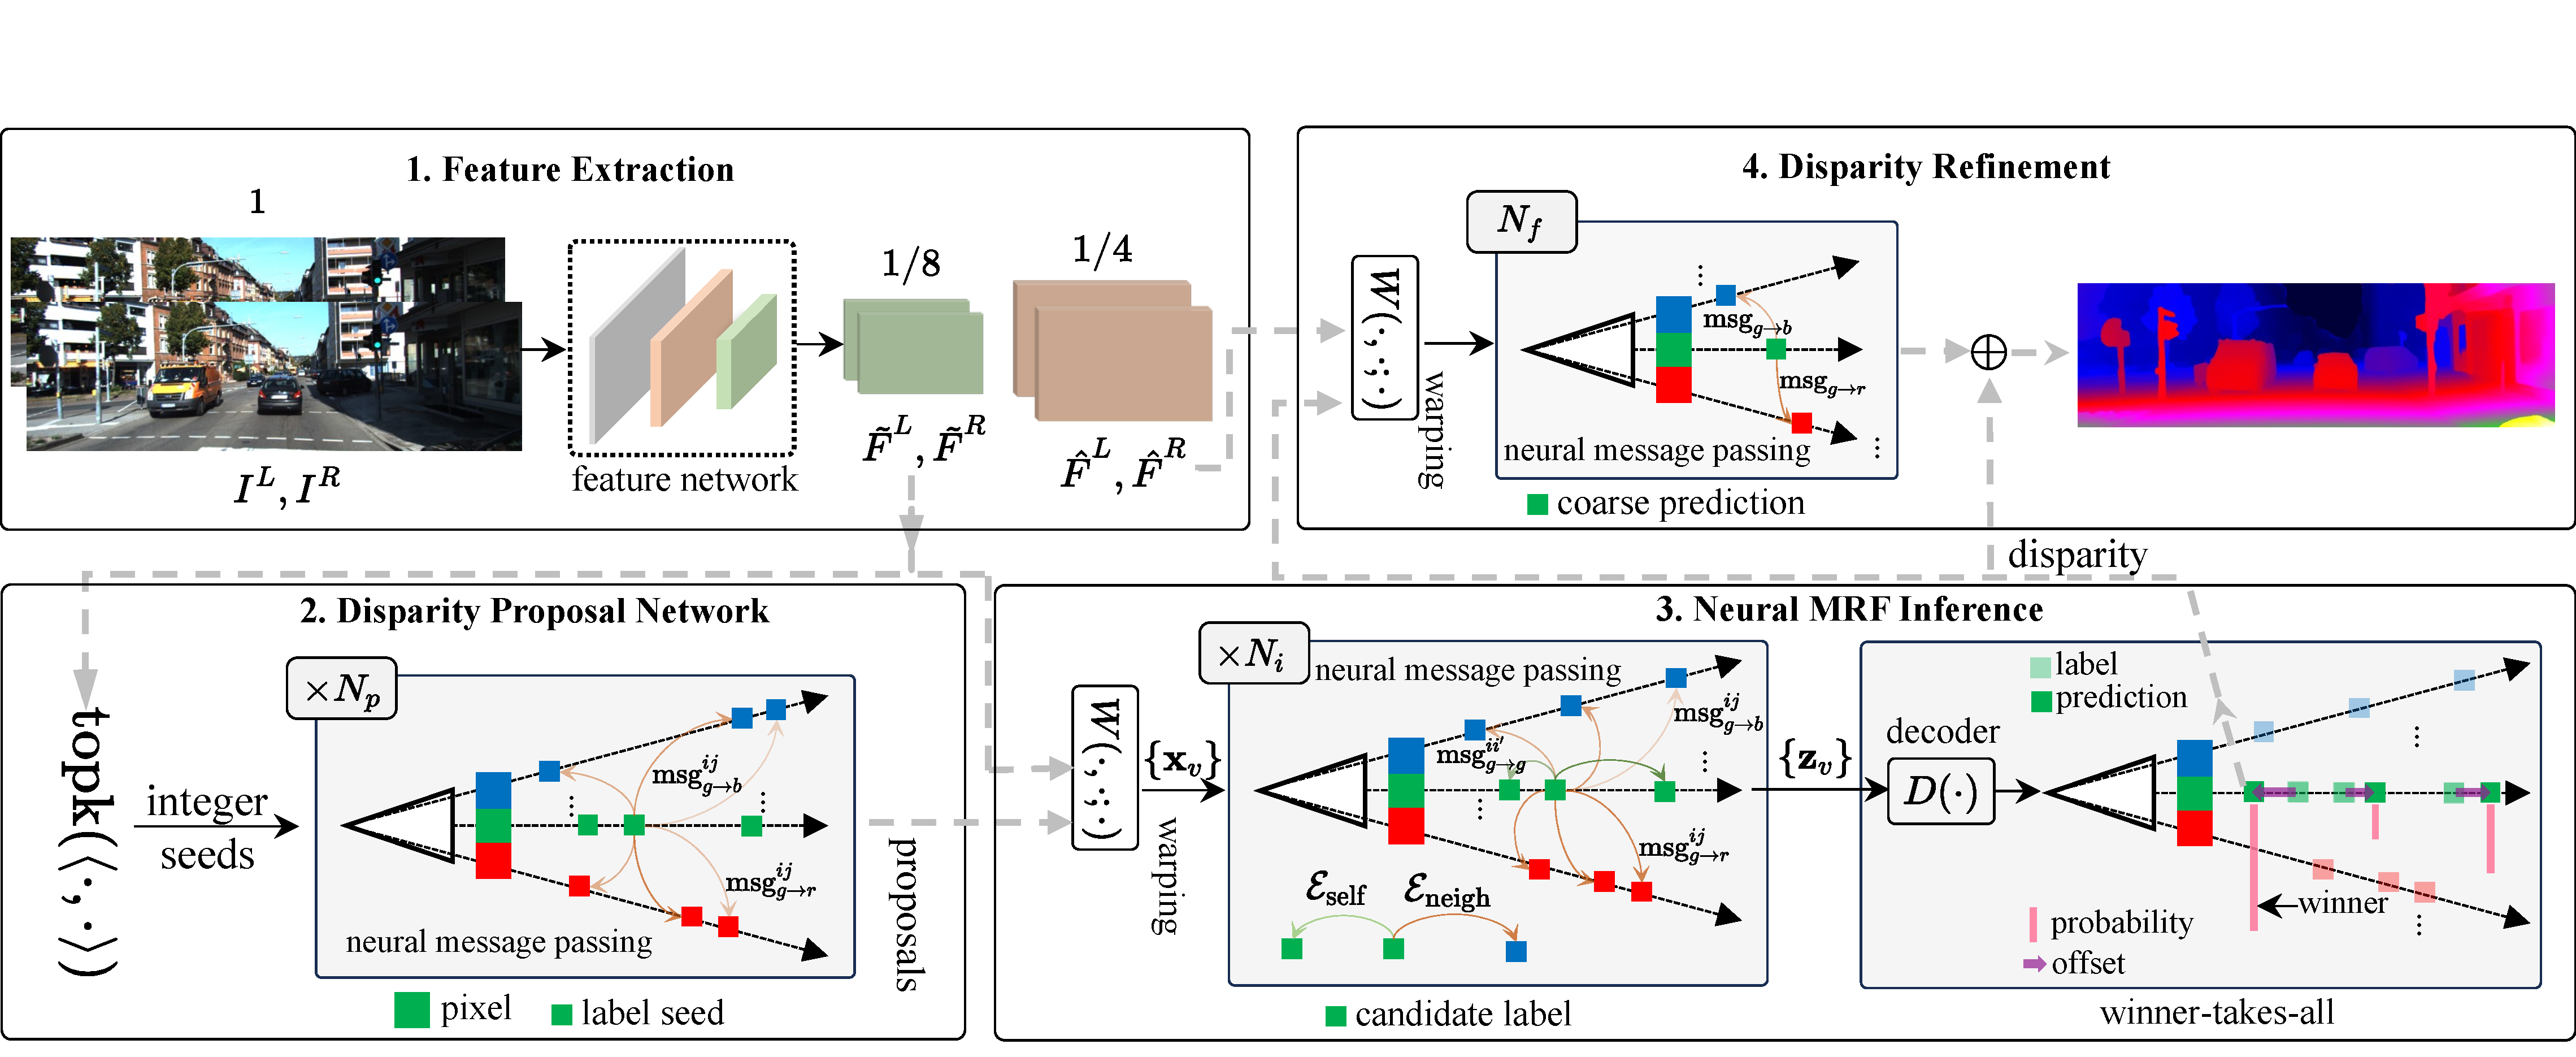
\includegraphics[width=0.99\linewidth]{fig/nmrf/overview.pdf}
	\vspace{-0.3em}
	\caption{\textbf{Architecture of the proposed NMRF model.} The pipeline consists of four submodules. \textbf{1.} A feature extraction network processes the input stereo pair and produces both coarse- and fine-level feature maps. 
		\textbf{2.} A disparity proposal network prunes the search space by selecting the top-$k$ candidate disparity modals for each pixel, which are further refined through $N_p$ iterations of neural message passing, yielding $k$ candidate disparity labels per pixel.
		\textbf{3.} These candidates are organized into a probabilistic graph, where each node represents a candidate label and edges connect labels across neighboring pixels. Distinct potential functions are employed for intra- and inter-pixel interactions. The latent embeddings $\{\mathbf{z}_v\}$  for each pixel are then decoded into posterior probabilities and offsets, from which the most likely label is selected as the coarse disparity estimate.
		\textbf{4.} A subsequent refinement applies a lightweight neural MRF with a single label per pixel, where the inferred embeddings are used to predict residual corrections for the final disparity.}
		\label{fig:nmrf_overview}
		\vspace{-0.2em}
\end{figure}
This section presents the implementation of the Neural Markov Random Field (NMRF) framework introduced in Sections~\ref{sec:mrf-model} and~\ref{sec:mrf-inference}.
An overview of the full architecture is shown in Figure~\ref{fig:nmrf_overview}.
This model follows a  two-stage design. 
In the first stage, an NMRF is applied at a coarse spatial resolution ($\nicefrac{1}{8}$ of the input image size) to produce an initial disparity estimate (Section~\ref{sec:nmrf_inference_network}).
To ensure computational tractability, we introduce a Disparity Proposal Network that significantly prunes the search space (Section~\ref{sec:dpn}).
In the second stage, the coarse predictions is refined at a higher resolution ($\nicefrac{1}{4}$ of the input size) features using a lightweight NMRF. 
Both stages are supported by a shared feature extraction network that provides both coarse- and fine-level features.

\subsection{Feature Extraction}\label{sec:nmrf_backbone}
Given a rectified stereo pair $(I^L, I^R)$, we employ a Siamese feature extractor to compute hierarchical feature representations.
Specifically, coarse-level features at $\nicefrac{1}{8}$ resolution are denoted as $\tilde{F}^L$ and $\tilde{F}^R$, while fine-level features at $\nicefrac{1}{4}$ resolution are denoted as $\hat{F}^L$ and $\hat{F}^R$.
These features play a critical role in stereo matching, especially in addressing challenges posed by occlusions, textureless regions, and varying lighting conditions.
However, achieving more expressive feature representations typically entails increased computation overhead.
To address the latency requirements of diverse applications, two feature network variants are introduced to balance performance and efficiency.

\begin{figure}[!t]
	\centering
	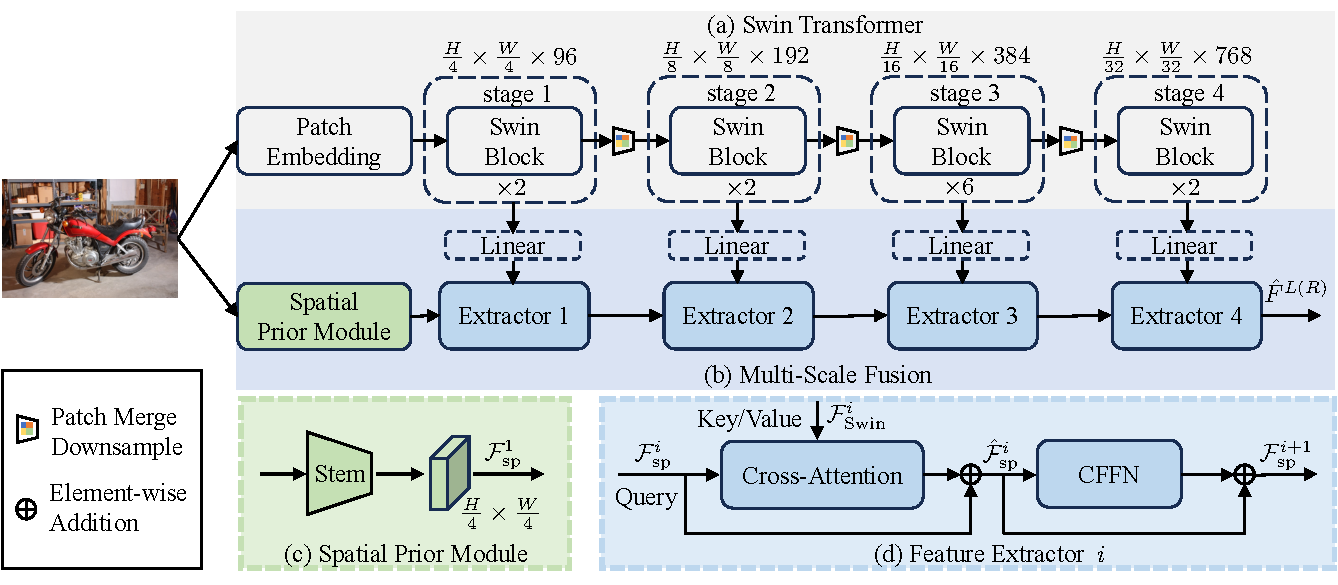
\includegraphics[width=0.99\linewidth]{fig/nmrf/backbone.pdf}
	\vspace{-0.3em}
	\caption{\textbf{Architecture of the performant feature network.} (a) The Swin-Tiny backbone, which produces hierarchical multi-scale features. (b) The multi-scale feature fusion strategy, which incorporates two key designs, including (c) a spatial prior module that captures local spatial contexts from the input image, and (d) a feature extractor that combines multi-scale features using the resolution-independent deformable attention~\cite{zhu2020deformable}.}
	\label{fig:nmrf_backbone}
	\vspace{-1.2em}
\end{figure}

\noindent\textbf{ResNet feature network.} For efficiency-critical settings, we adopt a lightweight convolutional backbone.
The input images $I^{L(R)} \in \mathbb{R}^{3 \times H \times W}$ are first downsampled to half resolution using a $7 \times 7$ convolution.
Feature extraction is then performed using a sequence of six residual blocks: two blocks at $\nicefrac{1}{2}$ resolution with 64 channels, followed by two blocks at $\nicefrac{1}{4}$ resolution with 96 channels, and two additional blocks at $\nicefrac{1}{4}$ resolution with 128 channels.
A final $1 \times 1$ convolution projects the features to obtain the fine-level representations $\hat{F}^L, \hat{F}^R \in \mathbb{R}^{256 \times \frac{H}{4} \times \frac{W}{4}}$.
The coarse-level features $\tilde{F}^L$ and $\tilde{F}^R$ are subsequently obtained by applying stride-2 average pooling to the fine-level features.
Instance normalization is used throughout the network to improve generalization performance~\cite{lipson2021raft}.

\noindent\textbf{Vision Transformer backbone}
To prioritize accuracy, we further explore feature extraction based on pre-trained vision transformers. Prior work~\cite{zhang2024exploring} has shown that transformer-based backbones, such as Swin~\cite{liu2021Swin} and Twins~\cite{chu2021twins}, provide stronger representations for stereo matching by leveraging rich instance-level semantics.
Motivated by this, we adopt an ImageNet-pretrained Swin-Tiny backbone and enhance it with a multi-scale feature fusion mechanism based on deformable attention, following ViT-Adaptor~\cite{chen2022vision} and Deformable Neck~\cite{zhang2024exploring}.
As illustrated in Figure~\ref{fig:nmrf_backbone}, the Swin backbone produces hierarchical features at multiple resolutions, which are progressively fused into a unified representation.

To strengthen local spatial modeling, we incorporate the Spatial Prior Module from ViT-Adaptor~\cite{chen2022vision}, which generates an initial feature map $\mathcal{F}_{\mathrm{sp}}^1$ containing fine-grained structural information.
This feature serves as the query in a sequence of deformable cross-attention layers.
At each stage, the spatial features are updated by attending to the corresponding Swin features:
\begin{align}
	\hat{\mathcal{F}}_{\mathrm{sp}}^i &= \mathcal{F}_{\mathrm{sp}}^i + \mathrm{Attention}\big(\mathrm{norm}(\mathcal{F}_{\mathrm{sp}}^i), \mathrm{norm}(\mathcal{F}_{\mathrm{Swin}}^i)\big)\\
	\mathcal{F}_{\mathrm{sp}}^{i+1} &= \hat{\mathcal{F}}_{\mathrm{sp}}^i + \mathrm{CFFN}\big(\mathrm{norm}(\hat{\mathcal{F}}_{\mathrm{sp}}^i)\big),
\end{align}
where $\mathcal{F}_{\mathrm{sp}}^i$ acts as the query, and $\mathcal{F}_{\mathrm{Swin}}^i$ provides the key and value. 
The convolutional feed-forward network (CFFN) uses a reduced expansion ratio of 0.25 to limit computational overhead.
The outputs from multi-scale fusion are used as the fine-level representations $\hat{F}^L, \hat{F}^R \in \mathbb{R}^{128 \times \frac{H}{4} \times \frac{W}{4}}$, while coarse-level features $\tilde{F}^L, \tilde{F}^R$ are obtained via average pooling.

\subsection{Disparity Proposal Network}\label{sec:dpn}
Direct inference over the full disparity space is computationally prohibitive for the proposed NMRF inference (Section~\ref{sec:mrf-inference}) due to the large number of candidate labels per pixel. 
To make inference tractable, we introduce a Disparity Proposal Network (DPN) that adaptively reduces the search space by selecting a compact set of reliable disparity candidates for each pixel. 
The DPN first identifies a sparse collection of promising disparity hypotheses and subsequently refines them through neural message passing, yielding $K$ high-quality disparity proposals per pixel.

\noindent\textbf{Top-$K$  Label Seeds.}
For a pixel $o=(i,j)$, the initial matching score for an integer disparity $d \in [0, d_{\mathrm{max}}]$ is computed via feature correlation:
\begin{equation}
	\mathbf{C}(i,j,d)=\langle \tilde{F}^L(i,j), \tilde{F}^R(i,j-d)\rangle.
\end{equation}
Rather than densely evaluating all disparity candidates during subsequent inference, we first identify a sparse set of representative disparity modals. 
Specifically, local maxima along the disparity dimension are detected using one-dimensional max pooling with kernel size $3$, corresponding to a local neighborhood of $[-1,1]$. 
A \verb|topk| operation is then applied to select the $k$ most confident modals.
Each selected modal is represented as a \emph{label seed} $(\mathbf{p}, \mathbf{d})$, consisting of a 3D position $\mathbf{p}$ and an associated matching descriptor $\mathbf{d}$. The position is defined as
\begin{equation}
	\mathbf{p}_v := (i,j,d),
\end{equation}
which encodes the pixel coordinates together with the candidate disparity. 
The matching descriptor is designed to capture both local matching evidence and disparity-aware geometric cues:
\begin{equation}
	\mathbf{d}_v=
	\mathrm{Linear}
	\Big(
	\delta_1\big(L_d(\mathbf{C}(i,j,:))\big)
	\, || \,
	\mathrm{PE}(d)
	\Big),
\end{equation}
where $L_d$ extracts local cost features centered at disparity $d$, following the strategy of RAFT-Stereo~\cite{lipson2021raft}. 
The extracted features are first normalized through a two-layer feed-forward network $\delta_1$, and subsequently concatenated with the sinusoidal positional encoding of disparity $d$. 
A linear projection is then applied to fuse appearance and geometric information into a unified representation.

\begin{figure}[!t]
	\centering
	\begin{subfigure}[t]{0.25\linewidth}
		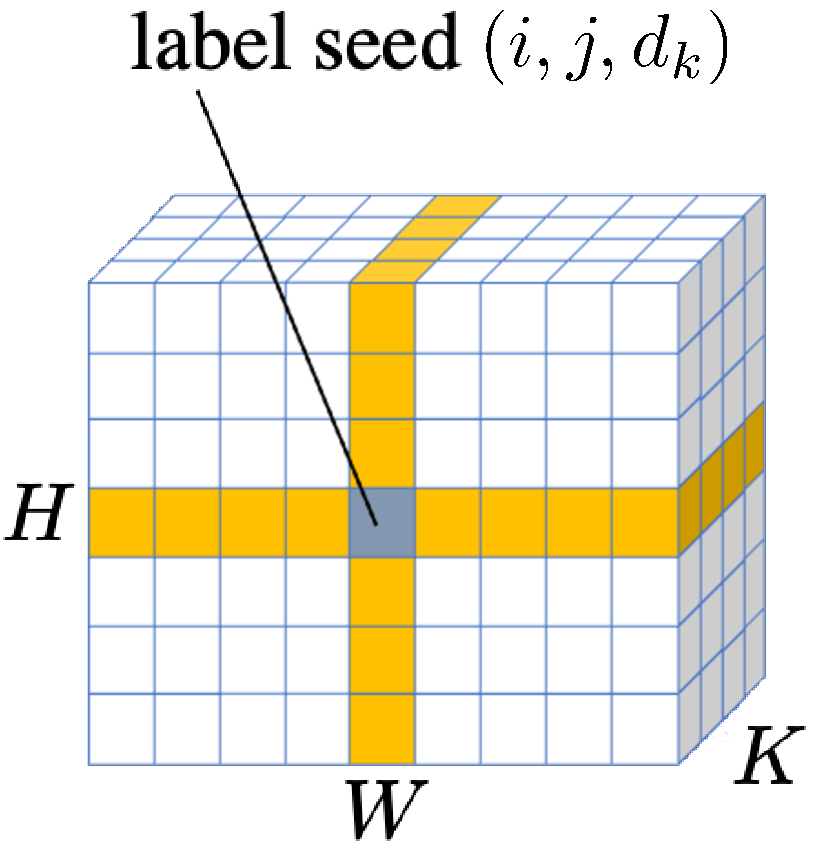
\includegraphics[width=\linewidth]{fig/nmrf/cross-shaped.pdf}
		\caption{}
		\label{fig:cross-shaped}
	\end{subfigure}
	\begin{subfigure}[t]{0.25\linewidth}
		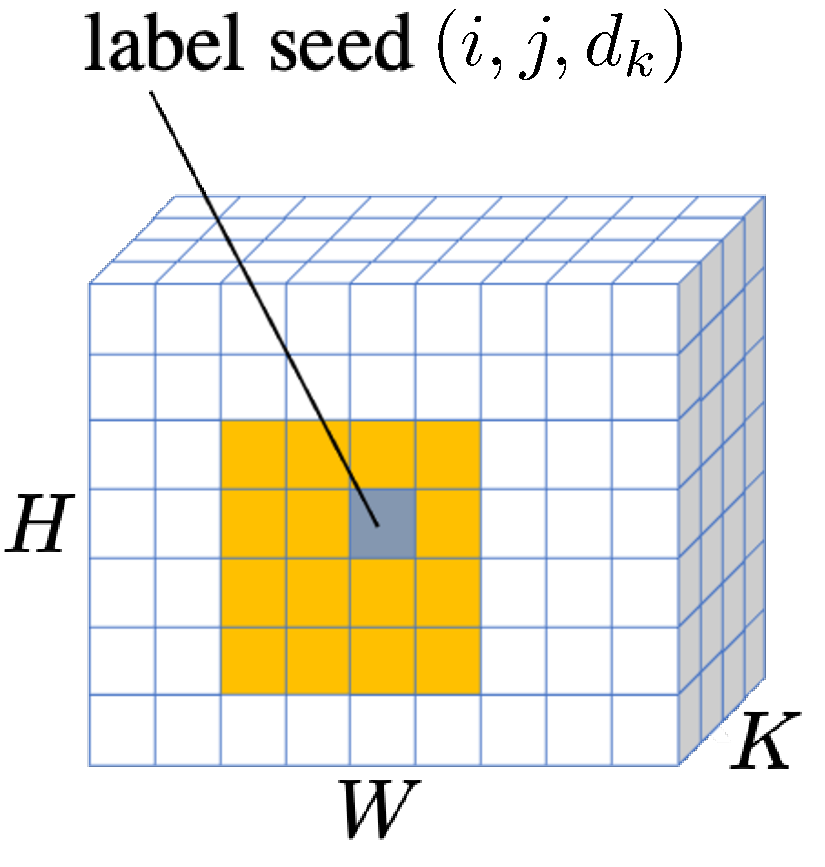
\includegraphics[width=\linewidth]{fig/nmrf/local-window.pdf}
		\caption{}
		\label{fig:local-win}
	\end{subfigure}
	\vspace{-1.0em}
	\caption{(a) Cross-shaped attention window layout, (b) local attention window layout.}  
	\vspace{-1.2em}
\end{figure}

\noindent\textbf{Label seed propagation.}
Although the top-$k$ label seeds provide strong initial hypotheses, they may still fail in challenging regions such as occlusions, reflective surfaces, or weakly textured areas. 
Nevertheless, correctly estimated seeds remain dominant across most parts of the image. 
This observation motivates the use of message passing to propagate reliable disparity cues toward ambiguous regions. 
Specifically, the neural message passing operation defined in Equation~\ref{eq:msg-passing} enables each label seed to incorporate contextual information from neighboring reliable hypotheses, thereby correcting erroneous or unstable disparity proposals.
Long-range interactions are particularly important for resolving large textureless regions and occluded areas. 
To efficiently capture such dependencies, we adopt the cross-shaped window self-attention mechanism of CSWin Transformer~\cite{dong2022cswin}. 
As shown in Figure~\ref{fig:cross-shaped}, a label seed located at $\mathbf{p}_v=(i,j,d)$ aggregates information from other seeds sharing either the same row index $i$ or column index $j$. 
This design enables efficient communication over large spatial extents while maintaining manageable computational complexity.
The propagation follows the \emph{parallel multi-head grouping} strategy and \emph{locally enhanced positional encoding} proposed in CSWin Transformer~\cite{dong2022cswin}.
In contrast to NMRF inference network (Section~\ref{sec:nmrf_inference_network}), the DPN excludes intra-pixel (\emph{self}) edges, since competition among candidate disparities is not required during proposal generation.
After $N_p$ iterations of message passing, the refined seed descriptors are decoded by a three-layer feed-forward network to predict residual corrections with respect to the initial integer disparity hypotheses.

To examine the effectiveness of the proposed cross-shaped attention design, we compare it with a conventional local window attention scheme illustrated in Figure~\ref{fig:local-win}.
For a fair comparison, the local attention window is configured to $8 \times 8$, resulting in a computational cost comparable to that of the cross-shaped attention on the SceneFlow dataset~\cite{mayer2016large} (\ie, $540\times 960$ resolution).
The quantitative comparison is presented in Table~\ref{tab:proposal_attention}.
The results indicate that cross-shaped attention yields more accurate disparity proposals, which can be attributed to its stronger capability for modeling long-range spatial dependencies during label seed propagation.

\subsection{Neural MRF Inference Network}\label{sec:nmrf_inference_network}
As illustrated in Figure~\ref{fig:nmrf_overview}(3), the NMRF inference network estimates the latent embeddings $\{\mathbf{z}_v\}$ from the observed label features $\{\mathbf{x}_v\}$ through $N_i$ iterations of neural message passing.
The resulting embeddings are subsequently decoded to produce disparity predictions.
While the general formulation of neural message passing has been introduced in Section~\ref{sec:mrf-inference}, this section describes the remaining components required for practical stereo inference.

\noindent\textbf{Observed Label Features.}
For each candidate label $v$ in the MRF graph, the observed feature $\mathbf{x}_v$ should jointly encode matching evidence from both stereo views.
Given the coarse-level feature maps $\tilde{F}^L$ and $\tilde{F}^R$, we construct the observed feature for a candidate located at $\mathbf{p}_v := (i,j,\hat{d})$ using a feature warping operation between $\tilde{F}^L(i,j)$ and $\tilde{F}^R(i,j-\hat{d})$:
\begin{align}
	\mathbf{x}_v
	&=
	\mathrm{MLP}
	\left(
	\mathbf{x}_v^{\mathrm{concat}}
	\, || \,
	\mathbf{x}_v^{\mathrm{corr}}
	\right), \nonumber \\
	\mathbf{x}_v^{\mathrm{concat}}(i,j,\hat{d})
	&=
	\delta_2\big(\tilde{F}^L(i,j)\big)
	\, || \,
	\delta_2\big(\tilde{F}^R(i,j-\hat{d})\big), \\
	\mathbf{x}_{v,g}^{\mathrm{corr}}(i,j,\hat{d},g)
	&=
	\frac{N_g}{N_c}
	\left\langle
	\delta_3\big(\tilde{F}_g^L(i,j)\big),
	\delta_3\big(\tilde{F}_g^R(i,j-\hat{d})\big)
	\right\rangle. \nonumber
\end{align}
Here, $\tilde{F}_g^L$ and $\tilde{F}_g^R$ denote the $g$-th feature groups obtained by evenly partitioning the coarse-level features into $N_g$ groups, while $N_c$ represents the total number of feature channels.
The term $\mathbf{x}_v^{\mathrm{concat}}$ captures appearance information through feature concatenation, whereas $\mathbf{x}_v^{\mathrm{corr}}$ measures matching similarity via grouped correlations.
The normalization functions $\delta_2$ and $\delta_3$ are introduced to align the feature distributions of the two components before fusion.
Both functions are implemented using a $3 \times 3$ convolution followed by instance normalization and ReLU activation, together with a subsequent $1 \times 1$ convolution layer.
Since the candidate disparity $\hat{d}$ may take continuous values after proposal refinement, bilinear interpolation is used when sampling the right-view feature map $\tilde{F}^R$.

\noindent\textbf{Disparity estimation.}
After $N_i$ iterations of neural message passing, the refined latent embeddings $\{^{(N_i)}\mu_v\}$ are decoded into disparity predictions.
For each coarse-level pixel, the embedding associated with every candidate label is processed independently to predict both disparity offsets and their corresponding confidence scores.
Specifically, a three-layer feed-forward network with ReLU activations regresses an $8 \times 8$ grid of disparity offsets relative to the candidate label. 
In parallel, a linear projection followed by a softmax operation estimates the posterior probability of each candidate. 
The predicted offsets are added to their associated candidate disparities, producing dense disparity hypotheses at the original image resolution.
Consequently, each input pixel $(i,j)$ is associated with a set of $K$ disparity hypotheses $\mathcal{H}_{ij}$, together with their estimated probabilities. 
The final disparity value is obtained using a winner-takes-all selection strategy, as illustrated in Figure~\ref{fig:nmrf_overview}(3).

\subsection{Disparity Refinement}\label{sec:nmrf_refinement}
The coarse-level NMRF inference already achieves strong performance, as demonstrated in Table~\ref{tab:ablation_comp}.
Nevertheless, fine-scale structures and object boundaries can be further improved through an additional refinement stage operating on higher-resolution features.
To this end, we perform $N_f$ iterations of neural message passing on the fine-level feature representations to refine the disparity estimation.
For computational efficiency, the refinement stage maintains only a single candidate label for each pixel.
The initial label is obtained by downsampling the coarse disparity prediction using stride-4 median pooling with a $4 \times 4$ kernel, producing a robust initialization at the fine feature resolution.
The resulting refinement graph differs from the coarse inference stage in two important aspects.
First, since each pixel contains only one disparity hypothesis, intra-pixel is no longer necessary, and therefore the graph contains no \emph{self} edges.
Second, the posterior probability prediction branch used during coarse inference is removed, as candidate selection is no longer required.
Consequently, the refinement stage focuses solely on propagating contextual information and predicting residual disparity corrections for enhanced structural detail.

\section{Loss Functions}
Our stereo network is trained end-to-end with losses applied to different stages of the pipeline, including label initialization, proposal extraction, multi-label MRF inference, and single-label disparity refinement.
These losses supervise complementary aspects of the model: the initialization loss encourages the cost volume to preserve plausible disparity modals, the proposal loss ensures that the extracted candidate labels cover the ground-truth disparity distribution within the local $8\times 8$ window, the multi-label disparity loss guides probabilistic MRF inference toward accurate hypotheses, and the refinement loss improves the final disparity accuracy.
Let $\Omega$ denote the set of valid pixels.
The overall training objective is defined as
\begin{equation}
	L_{\textsf{total}}
	=
	\lambda_{\textsf{init}} L^{\textsf{init}}
	+
	\lambda_{\textsf{prop}} L^{\textsf{prop}}
	+
	\lambda_{\textsf{disp}} L^{\textsf{disp}}
	+
	\lambda_{\textsf{ref}} L^{\textsf{ref}},
	\label{eq:total_loss}
\end{equation}
where $\lambda_{\textsf{init}}$, $\lambda_{\textsf{prop}}$, $\lambda_{\textsf{disp}}$, and $\lambda_{\textsf{ref}}$ balance the contributions of the four terms.
In our experiments, these weights are set empirically and kept fixed for all datasets unless otherwise specified.

\subsection{Initialization Loss}
The DPN first extracts label seeds from a 3D matching cost volume.
The purpose of the initialization loss is to encourage this cost volume to assign high responses to disparity modals that are likely to explain the local ground truth patch.
At the coarse resolution, each pixel $o$ corresponds to an image patch $\Omega_o$ in the original image.
Since $\Omega_o$ may contain multiple disparity modals, especially near object boundaries or thin structures, we construct a multi-modal target distribution from the valid disparities inside the patch.
Each valid disparity is first scaled to the coarse resolution by a factor of $8$, and then softly scattered to its two neighboring integer disparity bins using linear interpolation.
The scattered contributions from all valid pixels in $\Omega_o$  are accumulated and normalized into a probability distribution $\tilde{p}_o^*(d)$. 
Let $p_o(d)$ be the predicted disparity probability obtained by applying softmax to cost volume along the disparity dimension. 
The initialization loss is defined as the cross entropy between the patch-level soft target distribution and the predicted probability:
\begin{equation}
	L^{\textsf{init}}
	=
	-
	\frac{1}{|\Omega_{\textsf{init}}|}
	\sum_{o\in\Omega_{\textsf{init}}}
	\sum_{d=0}^{d_{\max}}
	\tilde{p}_o^*(d)
	\log p_o(d),
	\label{eq:init-loss}
\end{equation}
where $\Omega_{\textsf{init}}$ denotes the set of coarse-level pixels whose corresponding patch contains at least one valid ground truth disparity.
This soft cross-entropy loss encourages the initial cost volume to preserve the dominant disparity modals inside each local patch while still allowing secondary structures, boundary regions, and thin objects to contribute to seed selection.

\subsection{Proposal Loss}
While the initialization loss supervises the cost volume before seed selection, the proposal loss directly constraints the candidate labels after proposal extraction.
Let $L_o=\{\hat{d}_{o,k}\}_{k=1}^{K}$ be the set of candidate disparities proposed for coarse-level pixel $o$.
Ideally, these candidates should cover the ground-truth disparity values within the corresponding image patch $\Omega_o$.
For each valid pixel $p\in\Omega_o$, we identify the closest candidate label as
\begin{equation}
	\hat{\sigma}(p)
	=
	\arg\min_{k}
	\left| d_p^*-\hat{d}_{o,k} \right|.
	\label{eq:nearest-proposal}
\end{equation} 
The proposal loss is defined by minimizing the distance between each ground truth disparity and its nearest candidate:
\begin{equation}
	L^{\textsf{prop}}
	=
	\sum_o
	\sum_{p\in\Omega_o}
	\rho
	\left(
	d_p^*-\hat{d}_{o,\hat{\sigma}(p)}
	\right),
	\label{eq:l-prop}
\end{equation}
where $\rho(\cdot)$ denotes the Smooth-$L_1$ penalty.
This objective encourages the proposal network to generate a compact yet expressive set of candidate labels that can represent both smooth regions and locally multi-modal disparity structures.

\subsection{Multi-Label Disparity Loss}
After proposal extraction, neural MRF inference estimates a posterior distribution over the candidate disparity hypotheses. 
For pixel $(i,j)$, let $\mathcal{H}_{ij}$ denote the hypothesis set and let $p_{ij}(d')$ be the inferred posterior probability of hypothesis $d'\in\mathcal{H}_{ij}$. 
The multi-label disparity loss minimizes the expected absolute disparity error under this posterior distribution:
\begin{equation}
	L^{\textsf{disp}}
	=
	\sum_{(i,j)\in\Omega}
	\sum_{d'\in\mathcal{H}_{ij}}
	p_{ij}(d')
	\left| d'-d_{ij}^* \right|.
	\label{eq:loss-est}
\end{equation}
This loss favors posterior distributions whose probability mass is concentrated around accurate disparity hypotheses. 
Compared with supervising only the most likely label, the expectation-based formulation provides gradients to all hypotheses and therefore encourages both better probability estimation and more effective hypothesis refinement during neural message passing. 

\subsection{Refinement Loss}

The final refinement module predicts a continuous full-resolution disparity map $d$ from the output of coarse-level neural MRF inference. 
This stage is supervised using a direct regression loss between the refined disparity prediction and the ground-truth disparity map:
\begin{equation}
	L^{\textsf{ref}}
	=
	\sum_{(i,j)\in\Omega}
	\left|
	z_{ij}-z_{ij}^* 
	\right|.
	\label{eq:l-ref}
\end{equation}
This loss encourages the refinement module to recover fine-grained disparity details and sharpen local structures that may be smoothed in coarse-level multi-label inference.

\section{Experiments}
This section evaluates the proposed NMRF stereo framework from three perspectives: benchmark accuracy, cross-domain generalization, and component-level effectiveness.
To accommodate different computational requirements, two model variants are considered.
The efficiency-oriented variant, denoted as \emph{NMRF-light}, adopts the lightweight ResNet backbone introduced in Section~\ref{sec:nmrf_backbone} and maintains two candidate disparity labels for each pixel.
The accuracy-oriented variant denoted as \emph{NMRF-SwinT}, use the Swin Transformer~\cite{liu2021Swin} backbone described in Section~\ref{sec:nmrf_backbone} and retains four candidate labels per pixel.

Experiments are conducted on SceneFlow~\cite{mayer2016large}, KITTI~\cite{geiger2012we,menze2015object}.
SceneFlow is a large-scale synthetic stereo dataset containing 35,454 training pairs and 4,370 testing pairs with image resolution $540\times 960$ and dense ground-truth disparities.
KITTI 2012~\cite{geiger2012we} and KITTI 2015~\cite{menze2015object} are real-world autonomous driving benchmarks whose training sets provide sparse LiDAR-based disparity annotations.
KITTI 2012 contains 194 training pairs and 195 testing pairs, while KITTI 2015 contains 200 training pairs and 200 testing pairs.
For zero-shot evaluation, models trained only on SceneFlow are directly tested on the training splits of KITTI, Middlebury 2014~\cite{scharstein2014high}, and ETH3D~\cite{schops2017multi}.

\begin{table}[!t]
	\small
	\centering
	\caption{\textbf{Quantitative evaluation on SceneFlow test set.} Our NMRF-SwinT outperforms state-of-the-arts on both metrics.}
	\vspace{-0.6em}
	\resizebox{\linewidth}{!}{
	\begin{tabular}{c c c c c c c c c}
		\toprule 
		\textbf{Methods} & GANet~\cite{Zhang2019GANet} &  AANet~\cite{xu2020aanet} & 
		LEAStereo~\cite{cheng2020hierarchical} & ACVNet~\cite{xu2022attention} & IGEV-Stereo~\cite{xu2023iterative} & NMRF-light & NMRF-SwinT\\
		\midrule
		\textbf{EPE} [px] $\downarrow$ & 0.78 & 0.87 & 0.78 & 0.48 & 0.47 & 0.46 & \textbf{0.36}\\
		\textbf{Bad 1.0} [\%] $\downarrow$ &8.7&9.3&7.82&5.02&5.35&4.51&\textbf{3.64}\\
		\bottomrule
	\end{tabular}
	}
	\label{tab:results_sceneflow}
\end{table}

\subsection{Implementation Details}
All models are implemented in PyTorch and trained on NVIDIA RTX 3090 GPUs.
We use the AdamW optimizer together with a one-cycle learning-rate schedule for all training stages.
On SceneFlow, models are trained for 300k iterations with a batch size of 8.
Input images are randomly cropped to $384\times 768$, and the maximum learning rate is set to $5\times10^{-4}$.
Following the common SceneFlow evaluation protocol, pixels with ground-truth disparities larger than 192 are excluded during testing.
For KITTI benchmark submission, the SceneFlow pretrained model is further fine-tuned on the combined training images of KITTI 2012 and KITTI 2015.
Fine-tuning is performed for 39k iterations with a batch size of 4, using random crops of size $304\times 1152$ and a maximum learning rate of $2\times10^{-4}$.
Standard data augmentations are applied, including color jittering, eraser augmentation, and spatial transformation~\cite{lipson2021raft}.
Unless otherwise stated, all variants follow the same optimization and augmentation settings to ensure fair comparison.

\subsection{Benchmark Evaluation}

\begin{table}[!t]
	\small
	\centering
	\caption{\textbf{Evaluation on KITTI 2012 and 2015.} On KITTI 2012, we report the bad-$x$ error, \ie, the percentage of pixels with disparity error larger than $x$ pixels, for both non-occluded regions (noc) and all regions (all), together with the EPE on non-occluded pixels. On KITTI 2015, we report the D1 error for background (BG), foreground (FG), and all pixels. The best result is shown in \textbf{bold}, and the second-best result is \underline{underlined}.}
	\vspace{-0.3em}
	\resizebox{\linewidth}{!}{
	\begin{tabular}{c c c c c c c c c c}
		\toprule
		& \multicolumn{5}{c}{KITTI 2012} & \multicolumn{3}{c}{KITTI 2015} &\\
		\cmidrule(lr){2-6}
		\cmidrule(lr){7-9}
		\textbf{Methods} & \multicolumn{2}{c}{\textbf{bad 2.0}} & \multicolumn{2}{c}{\textbf{bad 3.0}} & \textbf{EPE}  
		& \textbf{BG} & \textbf{FG} & \textbf{ALL} & \textbf{Runtime}\\
		\cmidrule(lr){2-3}
		\cmidrule(lr){4-5}
		& noc [\%] &  all [\%] &  noc [\%] &  all [\%] & noc [px] & \multicolumn{3}{c}{All Areas [\%]} & [s] \\
		\cmidrule(lr){1-6}
		\cmidrule(lr){7-10}
		GCNet~\cite{kendall2017end} & 2.71 & 3.46  & 1.77 & 2.30 & 0.6 &  2.21 & 6.16 &  2.87 & 0.9\\
		PSMNet~\cite{chang2018pyramid} & 2.44 & 3.01 & 1.49 & 1.89  & 0.5 & 1.86 & 4.62 &  2.32 & 0.41\\  
		GwcNet~\cite{guo2019group} & 2.16 & 2.71 & 1.32 & 1.70 & 0.5 & 1.74 & 3.93 & 2.11 & 0.32\\
		GANet-deep~\cite{Zhang2019GANet}  & 1.89 & 2.50 & 1.19 & 1.60 &\textbf{0.4}      &1.48 &3.46 & 1.81 & 1.8 \\
		CSPN~\cite{cheng2019learning} & 1.79 & 2.27 & 1.19 & 1.53 & - & 1.51 & \underline{2.88} & 1.74 & 1.0\\
		RAFT-Stereo~\cite{lipson2021raft} & 1.92 & 2.42 & 1.30 & 1.66 & \textbf{0.4} & 1.58 & 3.05 & 1.82 & 0.38\\
		LEAStereo~\cite{cheng2020hierarchical} & 1.90 & 2.39 & 1.13 & 1.45 & 0.5 & 1.40 & 2.91 & 1.65 & 0.3\\
		ACVNet~\cite{xu2022attention} & 1.83 & 2.35 & 1.13 & 1.47 & \textbf{0.4} & 1.37 & 3.07 & 1.65 & 0.2\\
		IGEV-Stereo~\cite{xu2023iterative} & 1.71 & 2.17 & 1.12 & 1.44 & \textbf{0.4} & 1.38 & \textbf{2.67} & \textbf{1.59} & 0.18\\
		PCWNet~\cite{shen2022pcw} & 1.69 & 2.18 & \underline{1.04} & \underline{1.37} & \textbf{0.4} & 1.37 & 3.16 & 1.67 & 0.44\\
		\cmidrule(lr){1-6}
		\cmidrule(lr){7-10}
		PBCP~\cite{seki2016patch} & 3.63 & 5.01 & 2.36 & 3.45 & 0.7 & 2.58 & 8.74 & 3.61 & 68\\
		LBPS~\cite{knobelreiter2020belief} & - & - & - & - & - & 2.85 & 6.35 & 3.44 & 0.39\\ 
		NMRF-light (Ours) & \underline{1.64} & \underline{2.11} & 1.06 & 1.38 & \textbf{0.4} & \underline{1.30} & 3.29 & 1.63 & 0.05\\
		NMRF-SwinT (Ours) & \textbf{1.42} & \textbf{1.85} & \textbf{0.92} & \textbf{1.20} & \textbf{0.4} & \textbf{1.20} & \textbf{2.67} & \textbf{1.45} & 0.11\\
		\bottomrule
	\end{tabular}
	}
	\vspace{-0.5em}
	\label{tab:results_kitti}
\end{table}

We first compare the proposed models with representative stereo matching methods on SceneFlow finalpass, KITTI 2012, and KITTI 2015.
For SceneFlow, we report average end-point error (EPE) and the percentage of pixels whose disparity error exceeds one pixel, denoted as Bad 1.0.
As shown in Table~\ref{tab:results_sceneflow}, \emph{NMRF-SwinT} achieves superior accuracy under both metrics.
In particular, it reduces the Bad 1.0 error by 53.5\% compared with LEAStereo~\cite{cheng2020hierarchical} and by 32.0\% compared with IGEV-Stereo~\cite{xu2023iterative}.
Since these methods are representative of learned cost-volume aggregation and recurrent ConvGRU refinement, respectively, the comparison suggests that the proposed NMRF formulation provides an effective alternative for accurate disparity reasoning.

We further evaluate the models on the official KITTI 2012 and KITTI 2015 test sets.
The benchmark results are summarized in Table~\ref{tab:results_kitti}.
The proposed method achieves leading accuracy across the reported metrics on both KITTI benchmarks while maintaining competitive runtime.
Notably, the lightweight variant also obtains strong performance, demonstrating that the proposed architecture can be adapted to real-time or near-real-time deployment scenarios.
Compared with earlier learning-based MRF approaches, such as PBCP~\cite{seki2016patch} and LBPS~\cite{knobelreiter2020belief}, the proposed model provides substantially lower error rates, indicating the benefit of integrating structured probabilistic reasoning with modern neural feature learning.

\begin{figure}[!t]
	\centering
	\tabcolsep=0.02cm
	\begin{tabular}{c c}
		\raisebox{0.0em}{\rotatebox{90}{\scriptsize \textsf{NMRF-light} \hspace{0.1em} \textsf{LEAStereo} \hspace{0.6em} \textsf{Left Image}}} & 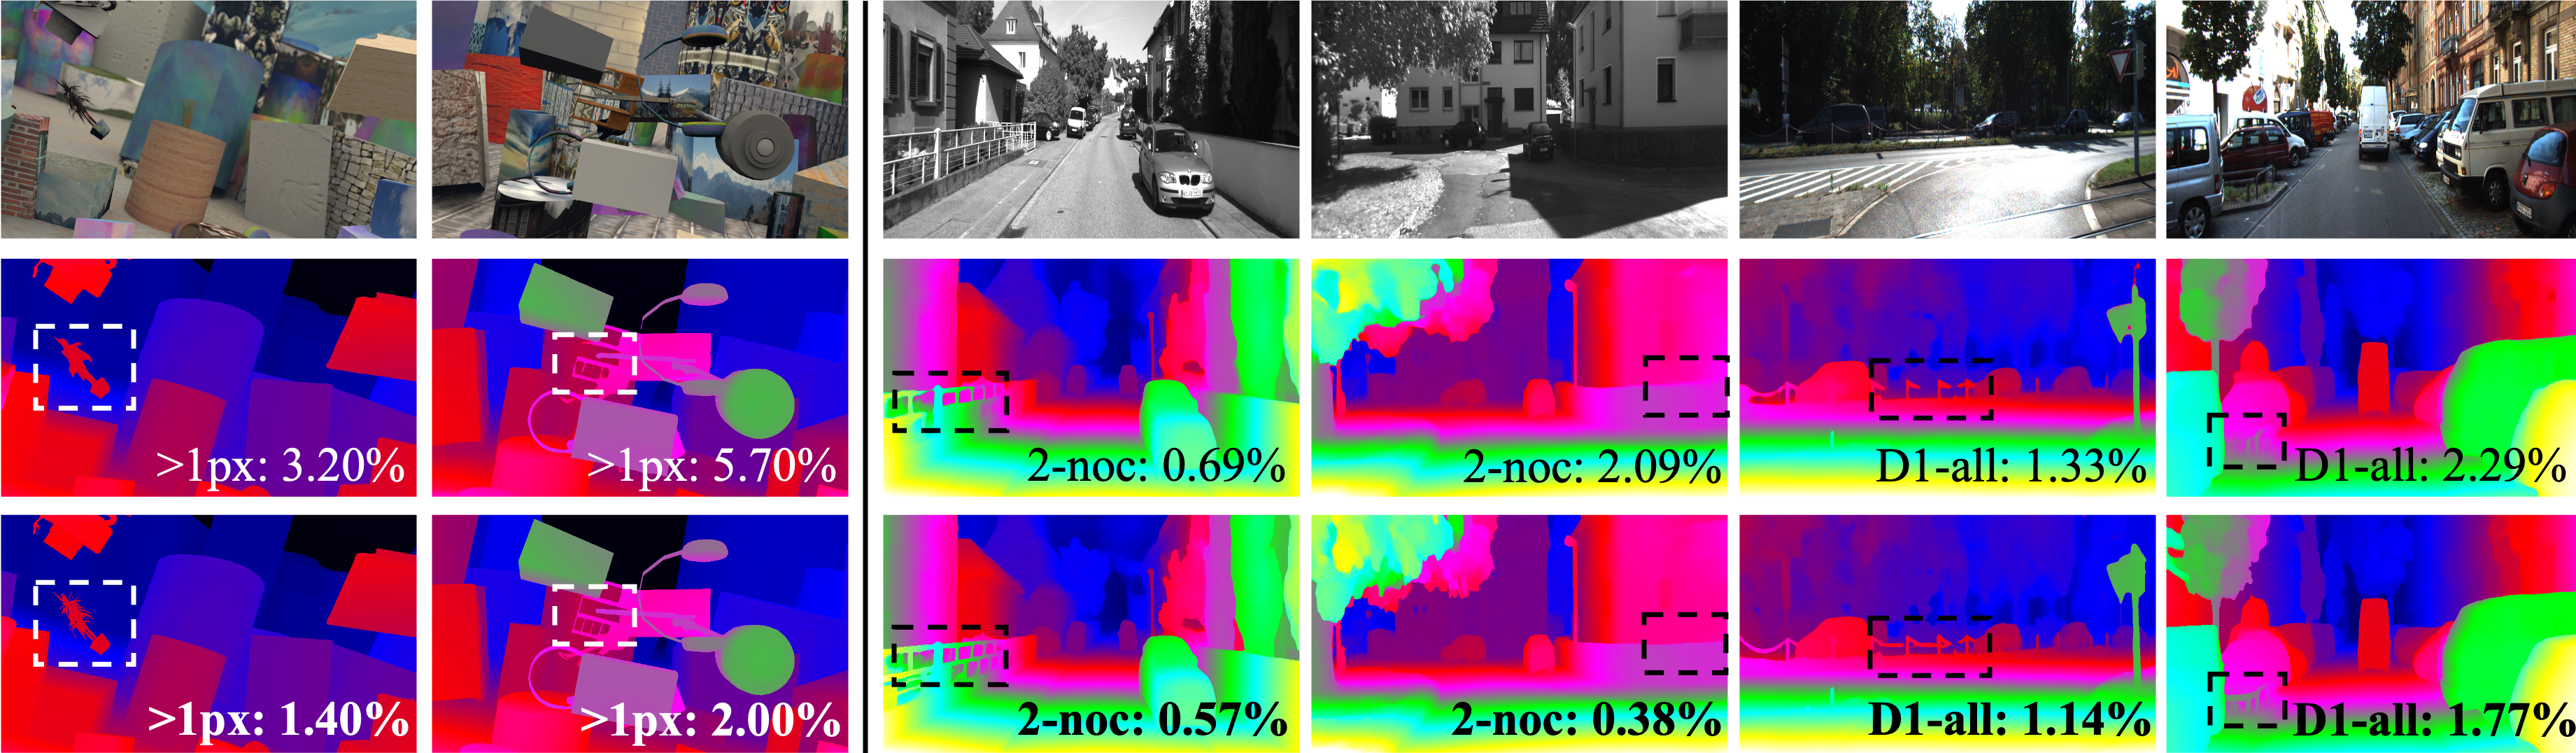
\includegraphics[width=0.97\linewidth]{fig/nmrf/sceneflow_kt.png}\\
	\end{tabular}
	\vspace{-0.8em}
	\caption{\textbf{Qualitative evaluation on SceneFlow~\cite{mayer2016large}, KITTI 2012~\cite{geiger2012we}, and KITTI 2015~\cite{menze2015object}.} Examples are organized from left to right as SceneFlow, KITTI 2012, and KITTI 2015, with two columns shown for each benchmark. The proposed method yields more coherent disparity predictions than LEAStereo~\cite{cheng2020hierarchical}, particularly in low-texture surfaces and regions containing fine geometric details.}
	\label{fig:sceneflow_kt}
	\vspace{-1.0em}
\end{figure}

Qualitative examples are shown in Figure~\ref{fig:sceneflow_kt}.
The predicted disparity maps preserve fine structures while remaining robust in low-texture regions.
To further examine boundary quality, we visualize reconstructed point clouds and compare them with those produced by LEAStereo~\cite{cheng2020hierarchical} and IGEV-Stereo~\cite{xu2023iterative}.
As illustrated in Figure~\ref{fig:nmrf_sharp}, the proposed method produces sharper discontinuities and substantially reduces bleeding artifacts~\cite{tosi2021smd}, which are particularly harmful for downstream 3D reconstruction and robotic perception.

\begin{figure}[!t]
	\centering
	\begin{subfigure}[t]{0.44\linewidth}
		\centering
		\tabcolsep=0.01cm
		\renewcommand*{\arraystretch}{0.35}
		\begin{tabular}{c c}
			\raisebox{0.0em}{\rotatebox{90}{\scriptsize \textsf{LEAStereo~\cite{cheng2020hierarchical}}}} 
			& 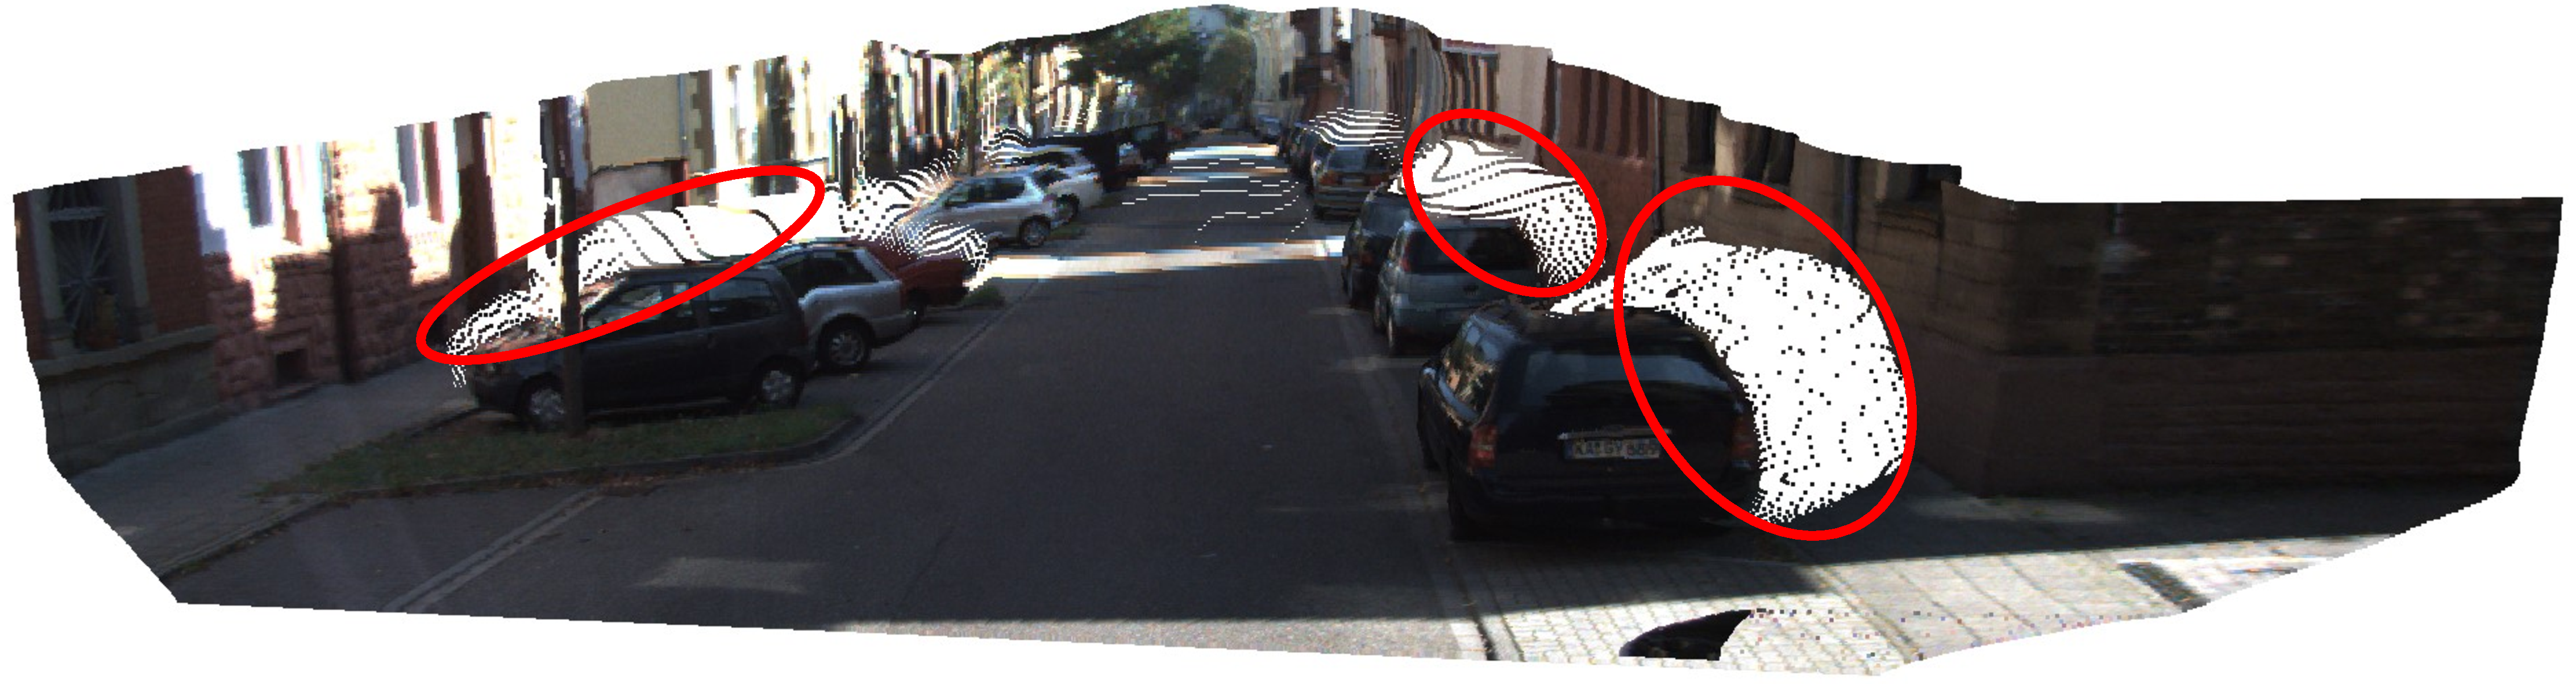
\includegraphics[width=0.88\linewidth]{fig/nmrf/leastereo.pdf} \\
			
			\raisebox{0.5em}{\rotatebox{90}{\scriptsize \textsf{IGEV~\cite{xu2023iterative}}}} 
			& 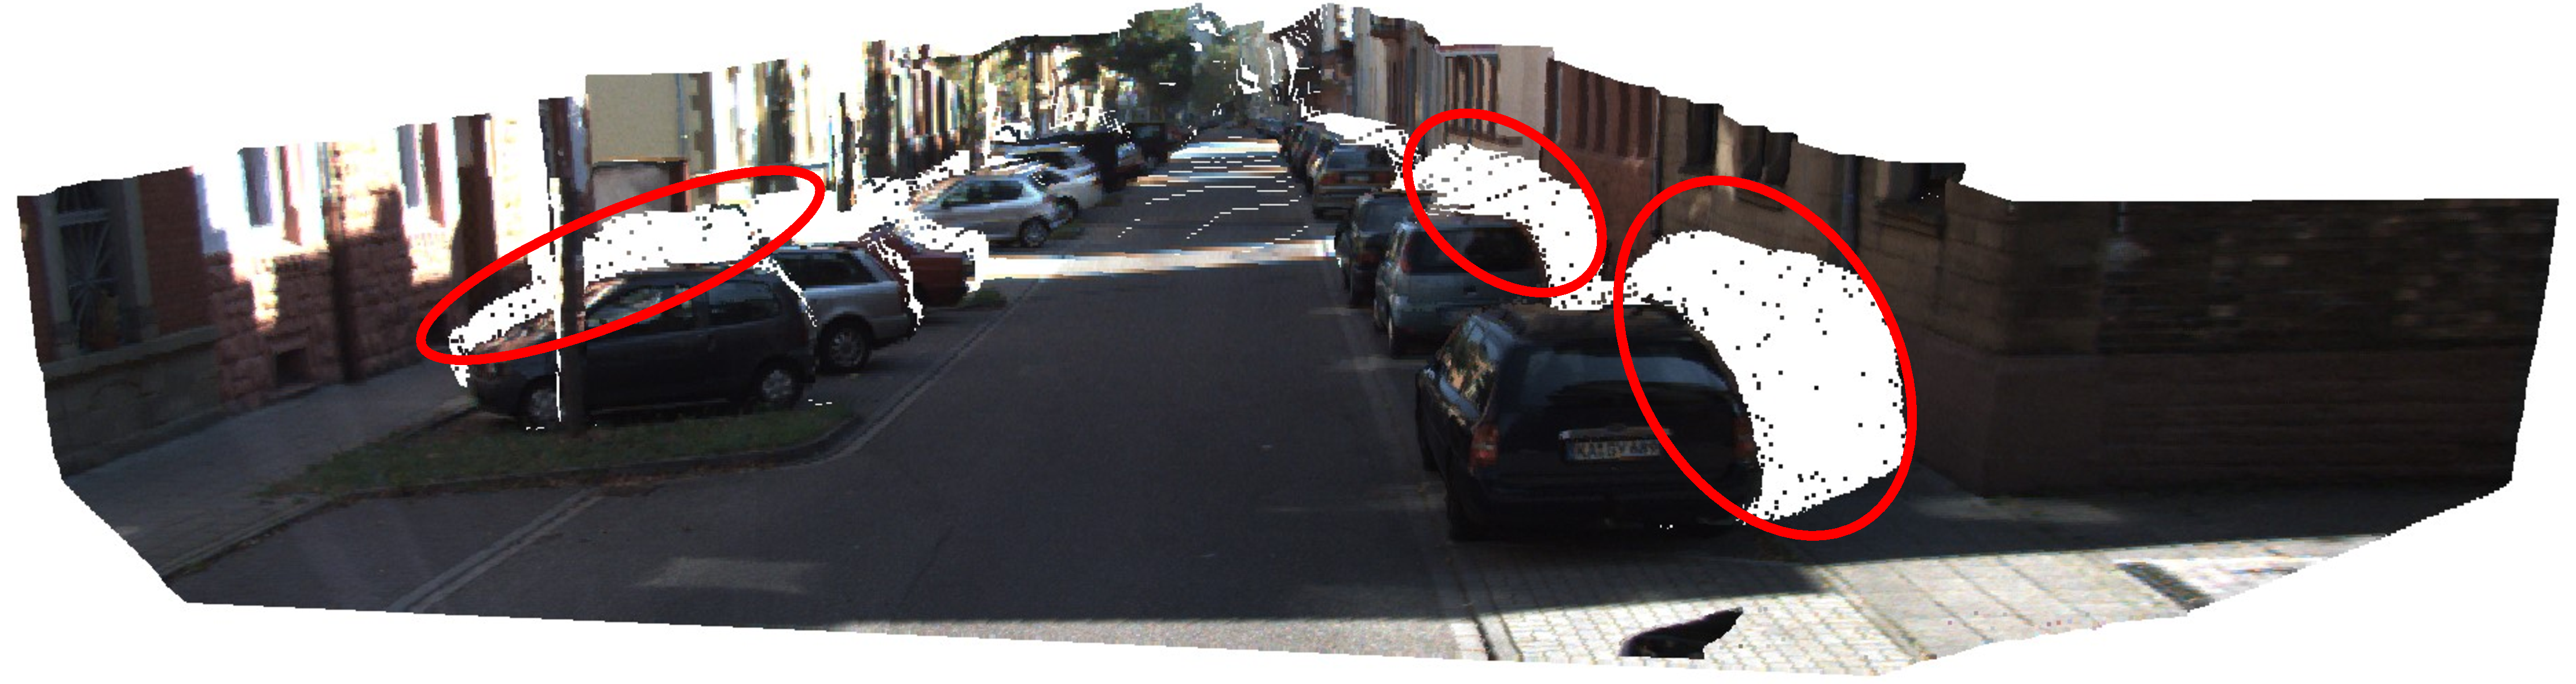
\includegraphics[width=0.88\linewidth]{fig/nmrf/igev.pdf} \\
			
			\raisebox{1.2em}{\rotatebox{90}{\scriptsize \textsf{Ours}}} 
			& 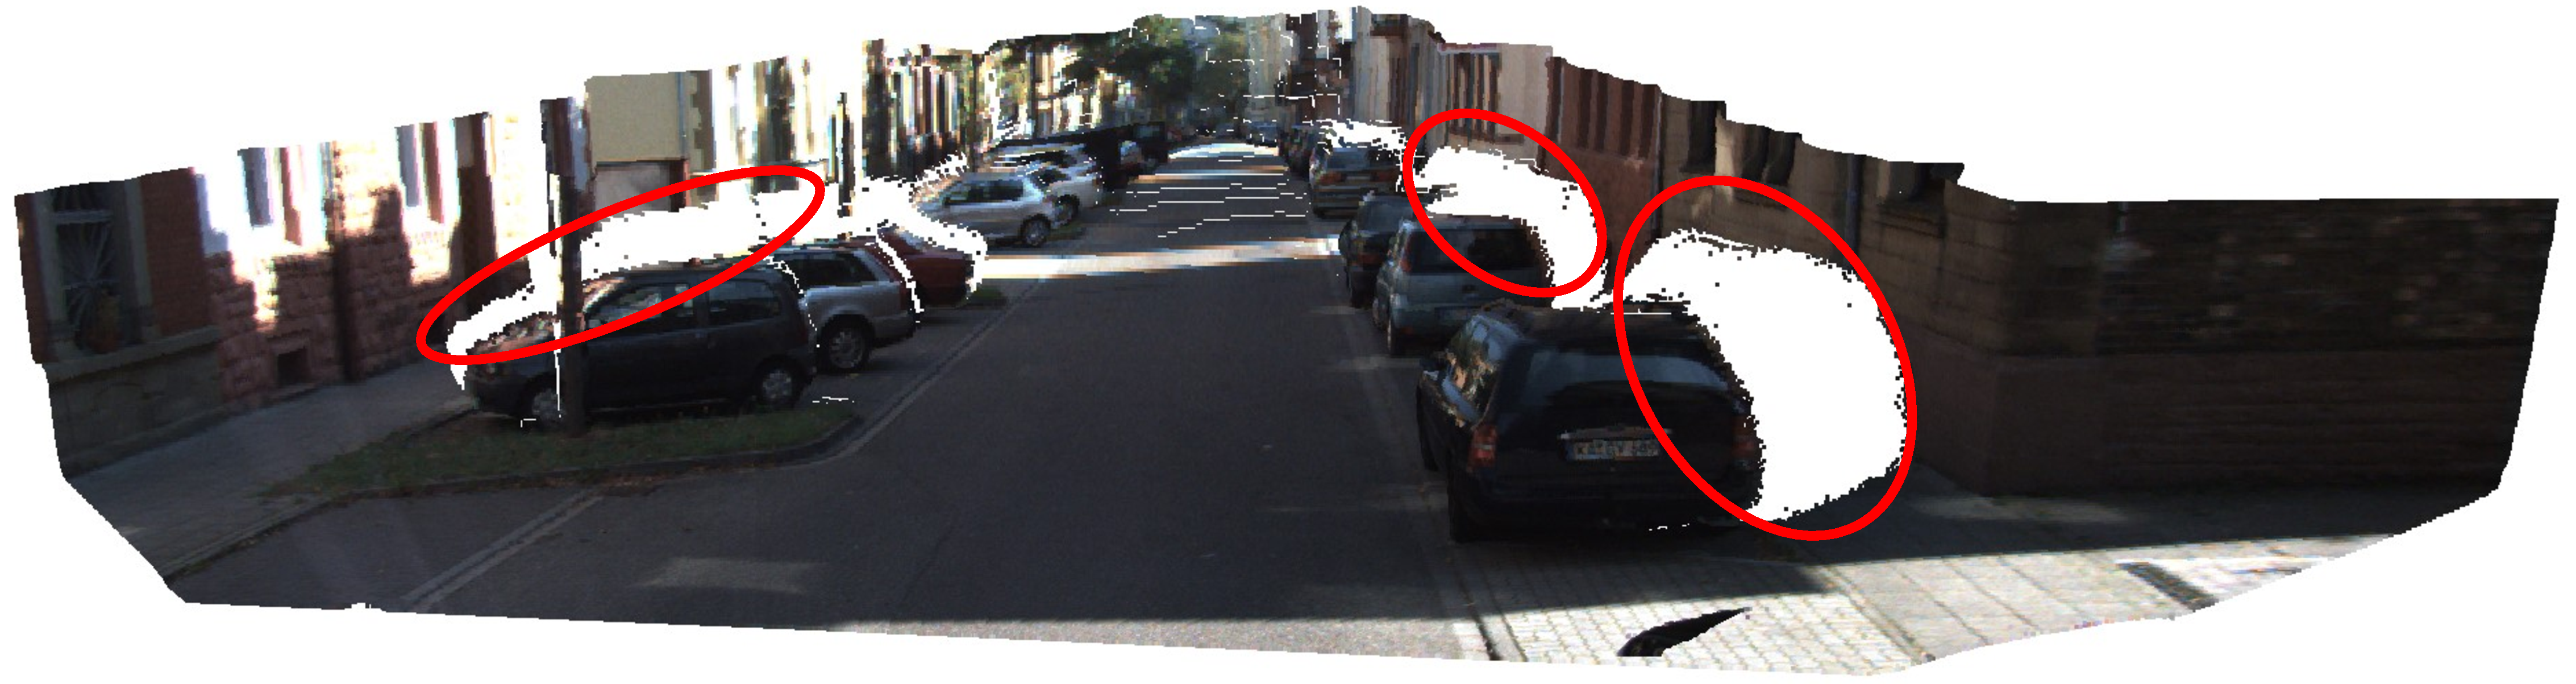
\includegraphics[width=0.88\linewidth]{fig/nmrf/nmrf.pdf}
		\end{tabular}
		\vspace{-0.2em}
		\caption{\small KITTI point-cloud reconstruction}
		\label{fig:nmrf_sharp}
	\end{subfigure}
	\hfill
	\begin{subfigure}[t]{0.55\linewidth}
		\centering
		\tabcolsep=0.01cm
		\renewcommand*{\arraystretch}{0.35}
		\begin{tabular}{c c}
			\raisebox{1.8em}{\rotatebox{90}{\scriptsize \textsf{Middlebury}}} 
			& 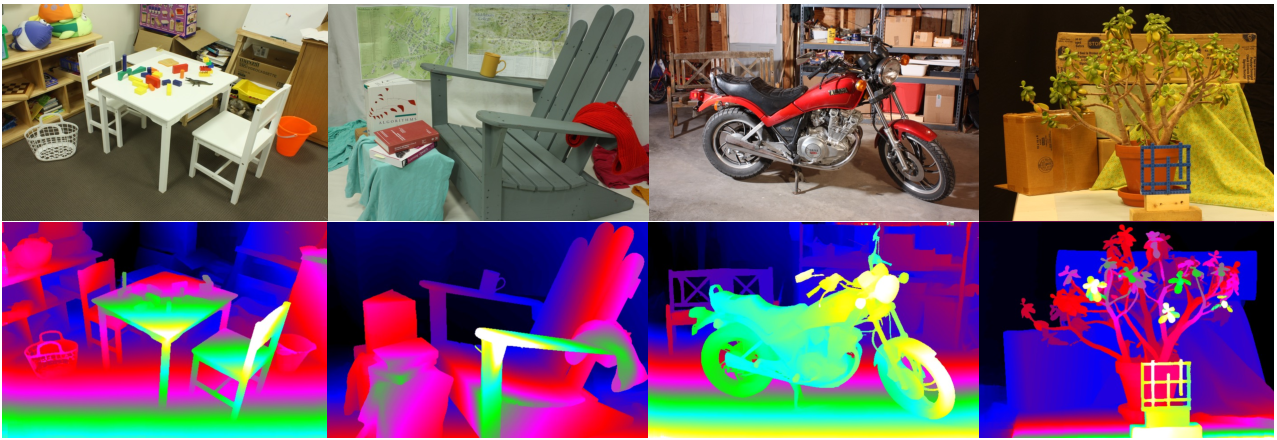
\includegraphics[width=0.88\linewidth]{fig/nmrf/middlebury.pdf} \\
			
			\raisebox{1.9em}{\rotatebox{90}{\scriptsize \textsf{ETH3D}}} 
			& 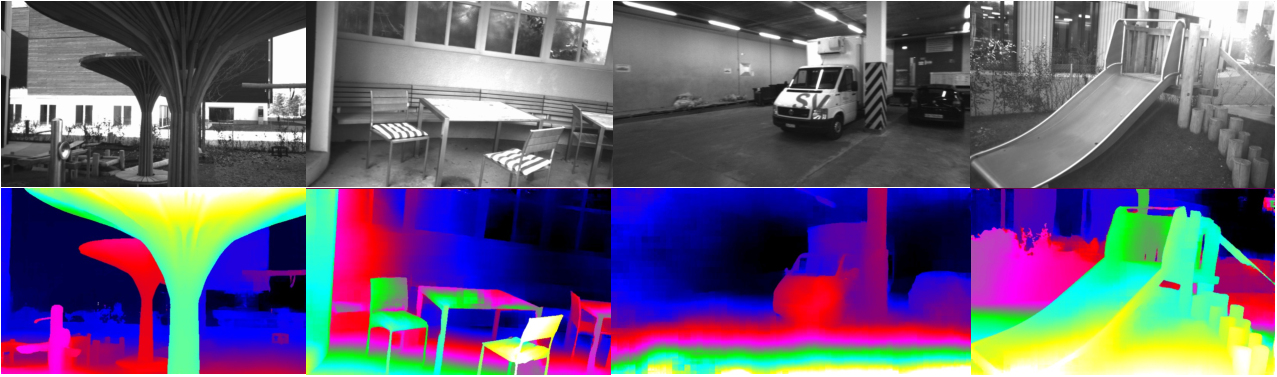
\includegraphics[width=0.88\linewidth]{fig/nmrf/eth3d.pdf}
		\end{tabular}
		
		\vspace{0.1em}
		\caption{\small Zero-shot generalization}
		\label{fig:qua-zero_shot}
	\end{subfigure}
	\vspace{-1.0em}
	\caption{\textbf{Qualitative evaluation of reconstruction quality and cross-dataset generalization.}
	(a) Point-cloud reconstruction results on the KITTI test set. Compared with LEAStereo~\cite{cheng2020hierarchical} and IGEV~\cite{xu2023iterative}, the proposed NMRF method produces sharper geometric boundaries and reduces bleeding artifacts around object contours.
	(b) Zero-shot qualitative results on Middlebury and ETH3D, demonstrating the generalization ability of the proposed method across datasets with different scene structures and imaging conditions.}
	\vspace{-0.5em}
\end{figure}

\subsection{Zero-Shot Generalization}

A stereo model trained on synthetic data should transfer reliably to real-world domains, since acquiring dense and accurate real-world disparity annotations is expensive and often impractical.
To assess this ability, we train models only on SceneFlow and directly evaluate them on KITTI, Middlebury, and ETH3D without any target-domain fine-tuning.
The quantitative results are reported in Table~\ref{tab:results_zero_shot}.
The proposed method demonstrates strong cross-domain robustness and outperforms DSMNet~\cite{zhang2020domain} and CREStereo++~\cite{jing2023uncertainty}, both of which are specifically designed to improve domain generalization.
This result indicates that the proposed candidate-label representation and neural MRF inference can capture transferable geometric structure rather than overfitting to synthetic appearance statistics.
The real-time \emph{NMRF-light} variant remains competitive, although its generalization performance is slightly lower than that of the original NMRF configuration.
Qualitative zero-shot results on ETH3D and Middlebury are provided in Figure~\ref{fig:qua-zero_shot}, showing that the model generalizes to diverse image conditions, including indoor scenes, grayscale images, and high-resolution stereo pairs.


\subsection{Ablation Studies}
We conduct ablation studies to analyze the contribution of the main architectural components.
For efficiency, all ablation experiments use the lightweight ResNet backbone unless otherwise specified.

\noindent\textbf{Effectiveness of the Disparity Proposal Network.} The quality of candidate labels is critical because the subsequent neural MRF inference is performed over the proposed hypothesis set.
If the correct disparity is not covered by any candidate, later message passing cannot fully recover it.
We therefore evaluate the Disparity Proposal Network (DPN) using two metrics.
The first is $x$-pixel recall, defined as the percentage of pixels for which at least one candidate label lies within $x$ pixels of the ground-truth disparity.
The second is the EPE between the ground-truth disparity and the closest candidate label.
As shown in Table~\ref{tab:proposal_quality}, the DPN significantly improves the quality of candidate hypotheses compared with the initialized label seeds.
At the 8-pixel threshold, corresponding to one pixel at the coarse feature resolution, the generated candidates achieve 99.8\% recall across commonly used datasets.
Moreover, the candidate-label EPE is substantially lower than the final disparity EPE, for example 0.22 versus 0.45 on SceneFlow.
These results demonstrate that the DPN provides a highly reliable hypothesis set and is unlikely to be the bottleneck of the overall framework.

\begin{table}[!t]
	\small
	\centering
	\caption{
	\textbf{Zero-shot generalization and ablation studies.}
	(a) zero-shot evaluation across KITTI 2012, KITTI 2015, Middlebury, and ETH3D. (b) ablation study on the SceneFlow test set.
	}
	\vspace{-1.0em}
	\begin{subtable}[t]{0.58\linewidth}
		\centering
		\scriptsize
		%\renewcommand{\arraystretch}{1.05}
		%\setlength{\tabcolsep}{1.8pt}
		\caption{\footnotesize Zero-shot generalization}
		\label{tab:results_zero_shot}
		\begin{tabular}{l c c c c}
			\toprule
			Method 
			& KITTI-12 
			& KITTI-15 
			& Midd. $\nicefrac{1}{4}$ 
			& ETH3D \\
			\midrule
			DSMNet~\cite{zhang2020domain} 
			& 6.2 & 6.5 & 8.1 & 6.2 \\
			RAFT-Stereo~\cite{lipson2021raft} 
			& 4.7 & 5.5 & 9.4 & \textbf{3.3} \\
			CREStereo++~\cite{jing2023uncertainty} 
			& 4.7 & \underline{5.2} & -- & 4.4 \\
			IGEV-Stereo~\cite{xu2023iterative} 
			& 5.2 & 5.7 & 8.8 & 4.0 \\
			\midrule
			NMRF 
			& \textbf{4.2} & \textbf{5.1} & \textbf{7.5} & 3.8 \\
			NMRF-light 
			& \underline{4.5} & 5.3 & \underline{8.0} & \underline{3.7} \\
			\bottomrule
		\end{tabular}
	\end{subtable}
	\hfill
	\begin{subtable}[t]{0.39\linewidth}
		\centering
		\scriptsize
		%\renewcommand{\arraystretch}{1.05}
		%\setlength{\tabcolsep}{2.0pt}
		\vspace{-0.5em}
		\caption{\footnotesize Component ablation}
		\label{tab:ablation_comp}
		\begin{tabular}{l c c c}
			\toprule
			Variant 
			& EPE 
			& Bad1.0 
			& Time \\
			\midrule
			baseline 
			& 0.58 & 5.96 & 0.064 \\
			w/ adaptive bias 
			& 0.57 & 5.80 & 0.067 \\
			w/ position aggregation 
			& 0.57 & 5.53 & 0.072 \\
			w/ \textit{shared} self edges 
			& 0.56 & 5.48 & 0.072 \\
			w/ self edges 
			& 0.53 & 5.24 & 0.081 \\
			\rowcolor{lightgray}
			w/ refinement 
			& 0.45 & 4.50 & 0.101 \\
			w/ refinement $\times 2$ 
			& 0.43 & 4.13 & 0.121 \\
			\bottomrule
		\end{tabular}
	\end{subtable}
\end{table}

\noindent\textbf{Number of candidate labels.} The number of candidate labels controls the trade-off between hypothesis diversity, computational cost, and inference stability.
In the main experiments, \emph{NMRF-light} uses two candidate labels per pixel, while \emph{NMRF-SwinT} uses four.
We further vary the number of labels $K$ to study its influence on accuracy, generalization, and runtime.
As shown in Figure~\ref{fig:k_boxplot}a, the model remains competitive even with a single candidate label, indicating that the proposal network often produces highly accurate hypotheses.
Increasing $K$ can improve candidate diversity, but the gain is not strictly monotonic.
When too many candidates are retained, inaccurate hypotheses may also enter the MRF inference stage and increase ambiguity.
For example, using six candidates does not consistently outperform using five.
Overall, $K=2$ offers a favorable accuracy-efficiency balance and is therefore adopted in the real-time model.

\begin{figure}[!t]
	\centering
	\vspace{1.5em}
	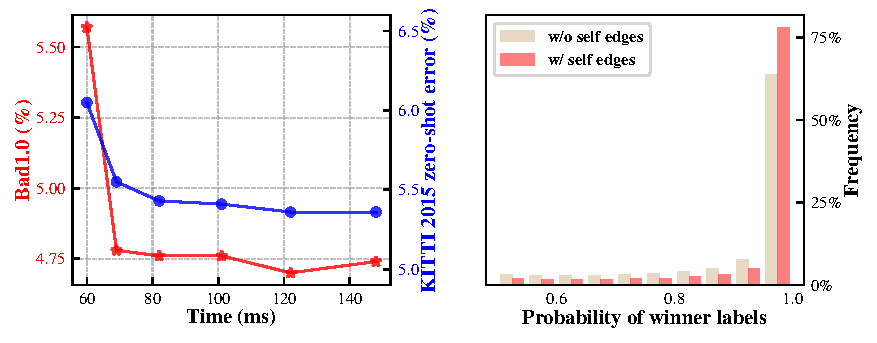
\includegraphics[width=0.96\linewidth]{fig/nmrf/ablation.pdf}\\
	\vspace{-0.2em}
	\makebox[0.5\linewidth]{\hspace{1em}\footnotesize (a)}
	\makebox[0.02\linewidth]{}
	\makebox[0.45\linewidth]{\hspace{-1em}\footnotesize (b)}\\
	\vspace{-0.5em}
	\caption{
		\textbf{Effect of candidate-label cardinality and self-edge propagation.}
		(a) Comparison of accuracy, inference time, and zero-shot generalization as the number of candidate labels varies from 1 to 6.
		(b) Histogram of the posterior probability associated with the winning label. Self-edge message passing makes the inferred label distributions more peaked, assigning higher probability to the selected candidate. The statistics are collected from 4.5M uniformly sampled pixels on the SceneFlow test set.
	}
	\label{fig:k_boxplot}
	\vspace{-1.0em}
\end{figure}

\noindent\textbf{Role of self edges.} We next study the role of self edges in neural MRF inference.
Unlike conventional stereo MRF formulations, where message passing is mainly defined between neighboring pixels, our model also allows information exchange among candidate labels belonging to the same pixel.
This design enables the network to reason about intra-pixel competition and reinforce the most plausible hypothesis.
As shown in Table~\ref{tab:ablation_comp}, including self edges improves disparity accuracy, reducing EPE from 0.57 to 0.53.
Figure~\ref{fig:k_boxplot}b depicts that self-edge message passing helps sharpen the posterior distribution over candidate labels and allows the loss in Equation~\ref{eq:loss-est} to more effectively emphasizing the selected hypothesis.
We also compare against a variant that shares the same potential function for self and neighboring edges ($4^{\mathrm{th}}$ row in Table~\ref{tab:ablation_comp}).
The performance drop of this shared-potential variant confirms that intra-pixel and spatial interactions should be modeled with distinct functions.

\noindent\textbf{Attentional aggregation components.} We further evaluate the two attentional aggregation designs in Equation~\ref{eq:nmrf_agg}: content-adaptive positional bias and position aggregation.
The results in Table~\ref{tab:ablation_comp} show that both components reduce disparity estimation outliers.
The content-adaptive positional bias is particularly beneficial around object boundaries, where aggregation should be sensitive to local appearance structure.
This behavior is consistent with the sharp discontinuities observed in Figure~\ref{fig:nmrf_sharp}.
Position aggregation, which injects positional information into the value branch, contributes more strongly to overall accuracy and improves predictions in broad textureless regions, as illustrated in Figure~\ref{fig:sceneflow_kt}.
Together, these two components make message aggregation both geometry-aware and content-adaptive.

\noindent\textbf{Disparity refinement.} Finally, we analyze the effect of the refinement module.
Among the components listed in Table~\ref{tab:ablation_comp}, the refinement module brings the largest performance gain.
This is expected because fine-level features at $\nicefrac{1}{4}$ resolution contain spatial details that are not fully preserved during coarse-level proposal extraction and MRF inference.
The refinement module therefore plays an important role in recovering thin structures, sharpening boundaries, and improving local disparity coherence.
Adding a second refinement module further improves in-domain accuracy but slightly weakens cross-domain generalization, as shown the last row of Table~\ref{tab:ablation_comp}.
This trade-off suggests that additional refinement can better fit the training distribution, while a simpler refinement design may preserve better robustness under domain shift.
In practice, the number of refinement stages can be chosen according to the target application, depending on whether maximum benchmark accuracy or stronger generalization is preferred.

\begin{table}[!t]
	\small
	\centering
	\caption{
		\textbf{Analysis of disparity proposal quality and seed propagation design.}
		(a) We evaluate the quality of the proposed disparity candidates on SceneFlow and KITTI validation splits. (b) We compare two attention patterns used for propagating label seeds. Candidate recall is measured by the percentage of pixels whose candidate set contains a label within a given threshold, while final disparity quality is measured by EPE and Bad 1.0.
	}
	\vspace{-0.5em}
	\begin{subtable}[t]{0.52\linewidth}
		\centering
		\scriptsize
		\caption{Quality of generated disparity candidates.
		}
		\label{tab:proposal_quality}
		\setlength{\tabcolsep}{2.2pt}
		\renewcommand{\arraystretch}{1.05}
		\begin{tabular}{c c c c c c}
			\toprule
			& \multicolumn{3}{c}{candidate labels} & \multicolumn{2}{c}{label seeds}\\
			\cmidrule(lr){2-4}
			\cmidrule(lr){5-6}
			Datasets & 3px & 8px & EPE & 8px & 16px \\
			& [\%]$\uparrow$ & [\%]$\uparrow$ & [px]$\downarrow$ & [\%]$\uparrow$ & [\%]$\uparrow$\\
			\cmidrule(lr){1-4}
			\cmidrule(lr){5-6}
			SceneFlow-test & 99.29 & 99.77 & 0.22 & 91.94 & 94.85\\
			KITTI-12 \textit{val} & 98.88 & 99.72 & 0.31 & 93.87 & 95.89\\
			KITTI-15 \textit{val} & 99.66 & 99.95 & 0.21 & 93.91 & 95.92\\
			\bottomrule
		\end{tabular}
	\end{subtable}
	\hfill
	\begin{subtable}[t]{0.44\linewidth}
		\centering
		\scriptsize
		\caption{Effect of the attention pattern for seed propagation.}
		\label{tab:proposal_attention}
		\setlength{\tabcolsep}{2.4pt}
		\renewcommand{\arraystretch}{1.05}
		\begin{tabular}{c c c c c c}
			\toprule
			& \multicolumn{2}{c}{candidate labels} & \multicolumn{2}{c}{disparity estimation}\\
			\cmidrule(lr){2-3}
			\cmidrule(lr){4-5}
			& 3px & 8px  & EPE & Bad 1.0 \\
			& [\%]$\uparrow$ & [\%]$\uparrow$ & [px]$\downarrow$ & [\%]$\downarrow$ \\
			\cmidrule(lr){1-3}
			\cmidrule(lr){4-5}
			cross-shaped & 99.29 & 99.77  & 0.45 & 4.50\\
			local window & 99.18 & 99.72 & 0.47 & 4.56 \\
			\bottomrule
		\end{tabular}
		
	\end{subtable}
	
	%\vspace{-0.5em}
	\label{tab:res_proposal}
	%\vspace{-1.7em}
\end{table}

\section{Application in Road Surface Perception}
The geometric profile of road surfaces critically impacts the driving performance of autonomous vehicles, as surface irregularities, such as bumps, potholes, and subtle elevation changes, can compromise vehicle stability, traction, and control.
Accurate, real-time perception of these features is essential for adaptive path planning, suspension control, and collision avoidance.
However, conventional sensing modalities face significant limitations in meeting the dual requirements of dense metric accuracy and operational robustness.
While LiDAR provides precise 3D measurements, its sparse point density (typically $< 100\,\mathrm{pt/m}^2$ at a $10\,\mathrm{m}$ range) limits its ability to capture fine-grained road elevation variations, such as cracks or shallow potholes with depths under $5\,\mathrm{cm}$.
Moreover, the high sensor cost and mechanical complexity of LiDAR hinder its widespread deployment in cost-sensitive applications.
Monocular depth estimation, although more cost-effective and lower in maintenance, faces challenges such as inherent scale ambiguity and instability in texture-scarce regions.
These issues are common to homogeneous paved roads, where elevation changes often lack distinct visual cues. Stereo vision addresses these gaps by providing dense, metric depth estimation at moderate cost, making it uniquely suited for detecting subtle road surface irregularities.
However, a critical challenge arises in this application: road surfaces often exhibit large textureless regions (\eg, uniform asphalt or concrete), where conventional stereo matching algorithms struggle due to insufficient intensity variations for reliable correspondence estimation.
Our NMRF architecture overcomes this limitation through long-range, data-dependent message passing, which propagates disparity hypotheses from geometrically confident regions (\eg, textured edges, lane markings) into textureless areas. 
Learned attention rules dynamically prioritize message from reliable neighbors, enabling the model to infer disparities via global structural reasoning rather than error-prone local matching.
For example, in flat road segments, the system synthesizes depth estimates by extrapolating cues from adjacent lane markings (top row of Figure~\ref{fig:road-ele}), effectively ``hallucinating'' plausible geometry where texture is absent.

To evaluate our architecture's road surface perception capability, we utilize the Road Surface Reconstruction Dataset (RSRD)~\cite{zhao2024road}, a specialized benchmark for road geometry analysis. 
RSRD contains 2,800 high-resolution stereo pairs ($1920 \times 1080$) with centimeter-level elevation ground truth derived from LiDAR-acquired disparities and 6-DoF poses.
The dataset focuses on diverse asphalt/concrete road conditions, including potholes, speed bumps, cracks, and subtle depressions, under varying illumination.
For texture-scarce evaluation, we adopt RoadBEV's~\cite{zhao2024roadbev} 1,210/371 train-test split at $960 \times 540$ resolution, prioritizing sequences with severe unevenness and minimal road markings. 
This configuration mirrors real-world challenges where homogeneous regions dominate and local textures are inadequate for conventional stereo matching. RSRD's sparse-texture, high-precision design provides a rigorous testbed for safety-critical automotive depth estimation systems.
For fair comparison, the evaluation region of interest (RoI) in Figure~\ref{fig:road-ele} aligns with the benchmark's prior work~\cite{zhao2024roadbev}, covering lateral and longitudinal ranges of $[-1.0\mathrm{m},0.9\mathrm{m}]$ and $[2.1\mathrm{m},7.1\mathrm{m}]$, respectively.
\begin{figure}[!t]
	\centering
	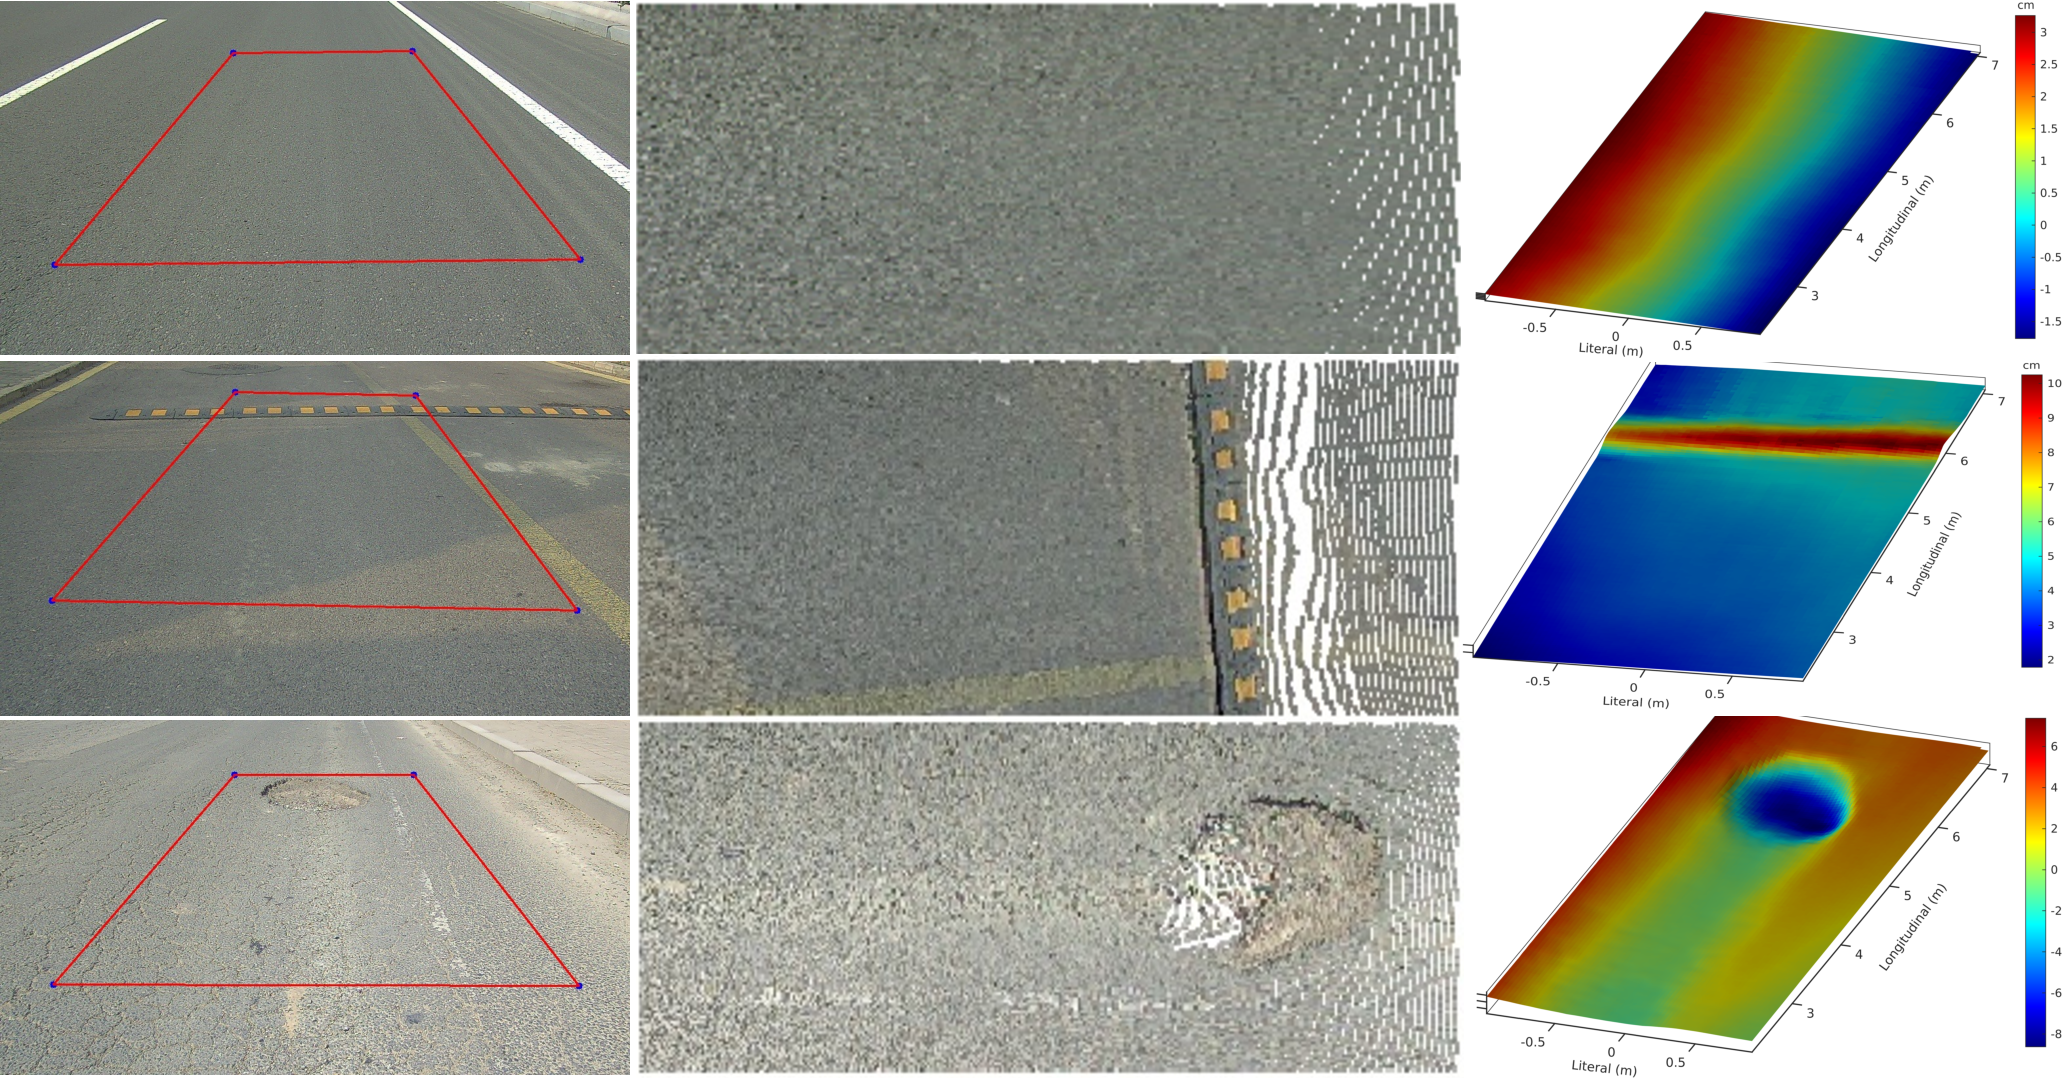
\includegraphics[width=0.99\linewidth]{fig/nmrf/elevation.pdf}
	%\vspace{-0.3em}
	\caption{\textbf{Visualization of road surface reconstruction using our method.} From left to right: left images, recovered road point clouds in a bird's-eye view, and estimated road meshes with colored elevation. Only the road surface within the region of interest (ROI) is visualized and evaluated.}
	\label{fig:road-ele}
\end{figure}

\section{Conclusion}
This chapter presented a neural Markov random field architecture for stereo matching.
Instead of relying on dense cost volume aggregation or recurrent ConvGRU refinement, the proposed method formulates stereo disparity estimation as structured inference over a compact set of candidate disparity labels.
This design retains the structural bias of classic MRF-based stereo methods while allowing the inference process to be learned end-to-end.
Experiments on synthetic and real-world benchmarks demonstrated strong accuracy, robust cross-domain generalization, and competitive efficiency. 
Within this thesis, this chapter establishes the stereo correspondence foundation for learning visual geometry, which will be extended in later chapters by incorporating additional sources of depth and motion cues.

\chapter{Structure-Aware Depth Completion for Robust Geometry Supervision}\label{ch:pseudo-label}
\section{Introduction}

Chapter~\ref{ch:nmrf} introduced Neural Markov Random Field (NMRF) as a structured neural inference framework for stereo matching.
By adaptively generating disparity hypotheses and refining them through neural message passing, NMRF enables efficient correspondence reasoning that resolves matching ambiguities while preserving sharp geometric discontinuities.
However, accurate depth learning depends not only on the model architecture, but also on the quality of ground-truth label.
In real-world robotic datasets, depth annotations are often sparse, noisy, and imperfectly aligned with the reference image.
These imperfections can significantly affect the geometry learned by stereo networks.

Outdoor stereo datasets commonly obtain depth annotations by projecting LiDAR measurements into the camera frame.
Although these measurements provide metric depth at sampled locations, the resulting labels are sparse in the image plane and usually suffer from sensor noise, calibration error, and temporal aggregation artifacts.
These issues are especially obvious near object boundaries, where projected labels can become spatially misaligned with the RGB image.
As a result, foreground objects may appear artificially thickened ($2^\mathrm{nd}$ row in Figure~\ref{fig:pseudo-labels}), thin structures may be removed, and small holes or fine details may be filled incorrectly.
When used directly as training targets, such labels can cause the network to reproduce the same artifacts, leading to blurred depth boundaries and degraded local 3D geometry.

This chapter addresses this supervision problem through structure-aware depth completion.
The goal is to convert sparse and noisy real-world depth annotations into denser and more reliable geometry supervision.
Rather than treating the available labels as fully accurate, we regard them as partial metric measurements that should be completed and corrected with the help of dense stereo prediction and image structure.
Specifically, an adapted NMRF model provides dense disparity estimates, confidence scores, and adaptive regularization weights, while the sparse labels provide metric anchors where measurements are available.
These sources are integrated by an optimization model that encourages local geometric coherence while preserving discontinuities aligned with image structures.
The completed labels are then used as additional supervision for training the stereo network.
This strategy is particularly useful near depth discontinuities and thin structures, where sparse LiDAR annotations are most likely to be unreliable.
Compared with direct training on sparse labels, structure-aware completion provides supervision that is denser, better aligned with visual boundaries, and less affected by annotation noise.
As a result, the trained model produces disparity maps with sharper boundaries and improved local surface quality.

The main contribution of this chapter are summarized as follows.
First, we analyze the effect of sparse and noisy real-world depth annotations on stereo learning, with particular attention to boundary thickening and degraded local geometry.
Second, we introduce a structure-aware depth completion formulation that combines sparse depth labels, dense NMRF predictions, confidence estimation, and image-guided geometric regularization.
Third, we show that the completed labels provide robust geometry supervision, improving disparity accuracy, boundary quality, and surface normal estimation under imperfect real-world annotations.

\section{From Sparse Labels to Robust Geometry Supervision}
Large-scale depth labels are essential for training modern stereo networks.
Synthetic datasets provide dense and accurate disparity labels, but their appearance statistics often differ from real-world scenes.
Real-world datasets better reflect deployment conditions, but their annotations are usually sparse and imperfect.
This creates a central tension in depth estimation: synthetic labels are geometrically accurate but visually less realistic, while real-world labels are visually relevant but often incomplete and noisy.
In autonomous driving datasets, depth labels are commonly obtained by projecting multi-frame aggregated LiDAR points into the camera frame.
Because LiDAR and cameras have different viewpoints and sampling pattern, the projected labels do not always align perfectly with image structures.
Moreover, many datasets increase label density by accumulating LiDAR scans across multiple frames.
Although this procedure provides more measurements, it also introduces errors when pose estimation, calibration, or dynamic-object handling is imperfect.
These errors often manifest as expanded object boundaries or misplaced depth discontinuities.
Such artifacts are harmful because depth prediction networks are trained imitate the provided supervision.
If a foreground object boundary is thickened in the label, the network may learn to predict a similarly expanded disparity pattern.
This produces bleeding artifacts in reconstructed point clouds and propagates errors to downstream 3D perception.
Therefore, robust depth learning requires not only a strong neural network, but also ground-truth depth labels that accurately captures the underlying scene geometry.
A natural remedy is to complete and refine sparse labels before using them for training.
However, depth completion is itself challenging.
Sparse measurements alone cannot determine dense geometry, while dense predictions from a pretrained network may fail under domain shift, occlusion, reflection, or weak texture.
The proposed approach resolves this ambiguity by combining both source within a structure-aware optimization framework.
Sparse labels provide metric constraints, dense NMRF predictions provide plausible geometry, and image-guided regularization encourages the completed depth to adhere to scene structure.

\section{Structure-Aware Depth Completion}
Given a rectified stereo image pair, let $d\in\mathbb{R}^{\Omega}_+$ denote the dense disparity predicted by a pretrained NMRF model over the image domain $\Omega$.
The model also predicts a confidence map $w\in[0,1]^{\Omega}$, where larger values indicate more reliable predictions.
In addition, an adaptive regularization weight $\alpha_1\in\mathbb{R}^{\Omega}_{+}$ is estimated to modulate the strength of local smoothness.
Let $d^{\mathrm{gt}}$ denote the sparse ground-truth disparity labels provided by the dataset.
Our goal is to estimate a completed disparity map $u\in\mathbb{R}^{\Omega}_+$ that satisfies three requirements.
It should preserve the metric information from available ground-truth sparse labels, remain close to reliable dense NMRF predictions, and maintain local geometric coherence without oversmoothing true depth discontinuities.
We formulate this objective as
\begin{equation}
	\min_{u}
	\;
	R(u; I^L)
	+
	G(u; d, w),
	\label{eq:sadc-energy}
\end{equation}
where $G(u;d,w)$ is a confidence-weighted data term and $R(u;I^L)$ is an image-aware geometric regularizer.

The dense NMRF prediction provides useful geometry in regions where sparse labels are unavailable.
However, these predictions should not be trusted uniformly.
We therefore weight their influence using the predicted confidence map:
\begin{equation}
	G(u; d, w)
	=
	\int_{\Omega}
	\frac{1}{2} w(x)
	\bigl(u(x)-d(x)\bigr)^2
	\mathrm{d}x .
	\label{eq:sadc-data}
\end{equation}
When $w(x)$ is high, the completed disparity is encouraged to follow the network prediction.
When $w(x)$ is low, the optimization relies more on sparse measurements and regularization.
During pseudo-label generation, available sparse labels are used as metric anchors so that the completed disparity remains consistent with real sensor measurements.

The regularization term is designed to encourage locally coherent geometry while preserving sharp boundaries.
We adopt a second-order Total Generalized Variation (TGV)~\cite{bredies2010total} prior:
\begin{equation}
	\mathrm{TGV}_{\alpha}^{2}(u)
	=
	\min_{\mathbf{v}}
	\left\{
	\alpha_1
	\int_{\Omega}
	|\nabla u-v| \mathrm{d}x
	+
	\alpha_0
	\int_{\Omega}
	|\nabla v| \mathrm{d}x
	\right\},
	\label{eq:sadc-tgv}
\end{equation}
where $\mathbf{v}$ is an auxiliary vector field that approximates the disparity gradient.
Compared with first-order smoothness, TGV better preserves piecewise affine surfaces, which are common in man-made environments.
Standard TGV does not consider image structure and may smooth across object boundaries.
To make the regularization aware of image structures, we introduce an anisotropic diffusion tensor derived from the left image:
\begin{equation}
	T
	=
	\exp
	\left(
	-\beta |\nabla I^L|^{\gamma}
	\right)
	nn^{\top}
	+
	n^{\perp}{n^{\perp}}^{\top},
	\label{eq:sadc-tensor}
\end{equation}
where $n=\nabla I^L/|\nabla I^L|$ denotes the image gradient direction, $n^{\perp}$ is its orthogonal counterpart, and $\beta$, $\gamma$ are hyperparameters controling the tensor's magnitude and sharpness.
This tensor suppress smoothing along the image gradient direction $n$ while promoting smoothness in the orthogonal direction $n^{\perp}$, to better align disparity transitions with image edges.
Combining the data term and the regularizer gives the final completion objective:
\begin{equation}
	\begin{aligned}
		\min_{u,v}
		\quad
		&
		\int_{\Omega} \alpha_1(x)
		|T(\nabla u-v)| \dd x
		+
		\alpha_0
		\int_{\Omega}
		|\nabla v| \dd x
		\\
		&
		+
		\int_{\Omega}
		\frac{1}{2}w(x)
		\bigl(u(x)-d(x)\bigr)^2 \dd x .
	\end{aligned}
	\label{eq:sadc-final-energy}
\end{equation}
The spatially varying weight $\alpha_1$ allows the regularization strength to adapt to local image and disparity structures.

\section{Primal-Dual Optimization}
The proposed optimization problem Equation~\ref{eq:sadc-final-energy} is convex but non-smooth due to the TGV regularizer.
To efficiently solve it, we adopt it through the first-order primal-dual algorithm proposed by~\cite{chambolle2011first}.
By introducing dual variables $p$ and $q$, the problem can be reformulated as a convex-concave saddle point problem using the Legendre-Fenchel transform:
\begin{equation}
	\begin{aligned}
		\min_{u,v}
		\max_{p\in\mathcal{P},q\in\mathcal{Q}}
		\quad
		&
		\alpha_1
		\langle T(\nabla u-v),p\rangle
		+
		\alpha_0
		\langle \nabla v,q\rangle
		\\
		&
		+
		\sum_{(i,j)\in\Omega}
		\frac{1}{2}w_{ij}(u_{ij}-d_{ij})^{2}.
	\end{aligned}
	\label{eq:sadc-saddle}
\end{equation}
Here $p$, $q$ are dual variables with feasible sets
\begin{equation}
	\mathcal{P}
	=
	\{p:\Omega\rightarrow\mathbb{R}^{2}
	\mid
	\|p_{ij}\|\leq 1\},
	\qquad
	\mathcal{Q}
	=
	\{q:\Omega\rightarrow\mathbb{R}^{4}
	\mid
	\|q_{ij}\|\leq \alpha_0\}.
\end{equation}
This reformulation enables iterative updates of primal and dual variables for each pixel.
Optimization proceeds via gradient-ascent on $q$ and $q$, followed by gradient-descent on $u$ and $v$.
Additionally, over-relaxation is applied to the primal variables to ensure convergence.

The variables are initialized as follows: $u^0=d$, $v^0=p^0=q^0=0$.
In practice, a fixed number of iterations is sufficient for generating pseudo labels.
Choose step size $\sigma_p>0$, $\sigma_q>0$, $\tau_u>0$, and $\tau_v>0$, the iterations proceed as:
\begin{equation}
	\begin{cases}
		p^{n+1}&=\mathcal{P}_p\left\{p^n+\sigma_p\alpha_1\left(T(\nabla \bar{u}^n-\bar{v}^n)\right)\right\}\\
		q^{n+1}&=\mathcal{P}_q\left\{q^n+\sigma_q \nabla \bar{v}^n\right\}\\
		u^{n+1}&=\frac{u^n+\tau_u\left(\alpha_1\nabla^\mathsf{T} Tp^{n+1} + wd\right)}{1 + \tau_u w}\\
		v^{n+1}&=v^n+\tau_v\left( \nabla^\mathsf{T} q^{n+1} + \alpha_1Tp^{n+1}\right)\\
		\bar{u}^{n+1}&=u^{n+1}+\theta (u^{n+1}-\bar{u}^n)\\
		\bar{v}^{n+1}&=v^{n+1}+\theta (v^{n+1}-\bar{v}^n)\\
	\end{cases}
	\label{eq:pd-step}
\end{equation}
The operators $\mathcal{P}_p$ and $\mathcal{P}_q$ perform pointwise Euclidean projection onto the feasible sets $P$ and $Q$:
\begin{equation}
	\mathcal{P}_p\{\tilde{p}_{i,j}\}=\frac{\tilde{p}_{i,j}}{\max(1, ||\tilde{p}_{i,j}||)},
	\mathcal{P}_q\{\tilde{q}_{i,j}\}=\frac{\tilde{q}_{i,j}}{\max(1, \nicefrac{||\tilde{q}_{i,j}||}{\alpha_0})}.
\end{equation}
We use a fixed relaxation parameter $\theta=1$.
The gradient operator $\nabla$ and divergence operator $\nabla^\mathsf{T}$ are discretized using forward and backward differences, with Neumann and Dirichlet boundary conditions applied where appropriate.

\section{Generating Pseudo Depth Labels}

The completed disparity map should be used for training only where it is sufficiently reliable.
Although dense NMRF predictions provide useful structure, they may still be inaccurate in regions with severe domain shift, occlusion, reflections, weak texture.
Therefore, pseudo-label generation should not simply densify sparse labels everywhere.
Instead, it should selectively combine reliable dense predictions with sparse metric measurements and discard regions where the completed geometry is insufficiently supported.

\subsection{Adapting NMRF for Completion}
To provide necessary cues for structure-aware depth completion, we slightly adapt the NMRF refinement module (Section~\ref{sec:nmrf_refinement}).
In addition to predicting the refined disparity map $d$, the network is extended to estimate two auxiliary maps: a confidence map $w$ and an adaptive regularization coefficient $\alpha_1$.
These maps are not used as final depth outputs.
Rather, they guide the depth completion process by determining where the dense prediction should be trusted and how strongly local smoothness should be imposed.

The confidence map $w\in[0,1]^{\Omega}$ measures the reliability of the dense disparity prediction.
A large value indicates that the prediction is likely to provide a useful constraint in the completion objective, while a small value weakens the influence of the network prediction.
For numeric stability, the network predicts an unconstrained variable $s$ and maps it to the confidence in log-space:
\begin{equation}
	w(x)=\exp\bigl(-s(x)\bigr),
	\qquad
	s(x)\in[0,10].
\end{equation}
This parameterization ensures positive confidence values and avoid numeric instability as we directly regress aleatoric uncertainty in log space.
The adaptive coefficient $\alpha_1$ controls the strength of the first-order term in the structure-aware regularizer.
Intuitively, large $\alpha_1$ encourages stronger local geometric coherence, while small $\alpha_1$ relaxes the smoothness constraint near likely discontinuities or complex structures.
The network predicts another variable $\zeta$ and maps it into a bounded interval:
\begin{equation}
	\alpha_1(x)
	=
	\alpha_1^{-}
	+
	\bigl(\alpha_1^{+}-\alpha_1^{-}\bigr)
	\sigma\bigl(\zeta(x)\bigr),
	\label{eq:sadc-alpha}
\end{equation}
where $\sigma(\cdot)$ denotes the sigmoid function, and $\alpha_1^{-}$ and $\alpha_1^{+}$ define the minimum and maximum regularization strengths.
In practice, these maps are decoded from the fine-level NMRF features using a lightweight prediction head parallel to the disparity residual head.
This design allows the completion model to use not only the disparity prediction itself, but also the network's estimate of prediction reliability and local geometric complexity.

With this adaption, the pretrained NMRF model provides three dense inputs for label generation:
\begin{equation}
	d,\; w,\; \alpha_1
	=
	f_{\mathrm{NMRF}}(I^L,I^R),
	\label{eq:sadc-nmrf-cues}
\end{equation}
where $d$ is the dense disparity prediction, $w$ is the confidence map, and $\alpha_1$ is the adaptive regularization coefficient.
These cues are then combined with the sparse real-world label $d^{\mathrm{gt}}$ in the structure-aware completion objective introduced in Equation~\ref{eq:sadc-final-energy}.
The confidence map $w$ and adaptive regularization coefficient $\alpha_1$ should provide meaningful cues for the structure-aware completion model.
To encourage this behavior, we introduce an auxiliary supervision signal by unrolling the primal-dual optimization steps in Equation~\ref{eq:pd-step}.
The unrolled solver is differentiable, allowing gradients to propagate through the completion process and update the NMRF branches that predict $d$, $w$, and $\alpha_1$.
Let $\hat{u}$ and $\hat{v}$ denote the outputs of the unrolled completion solver for the optimization problem.
Here, $\hat{u}$ is the completed disparity map, and $\hat{v}$ is the auxiliary field associated with local disparity variation.
A direct way to transfer the effect of the completion solver to NMRF would be to enforce consistency between the solver output $\hat{u}$ and the network prediction $d$, \ie, $|\hat{u}-d|$.
However, the completed output is not always more accurate than the network prediction.
In regions with complex non-planar geometry, very thin structures, or weak image evidence, the piecewise-affine regularization assumption may be imperfect and can over-smooth local details.
To make the auxiliary supervision robust, we anchor both the network prediction and the completed output to the available ground-truth disparity:
\begin{equation}
	L^{\textsf{aux}}
	=
	\frac{1}{|\Omega|}
	\sum_{(i,j)\in\Omega}
	\left(
	|\hat{u}_{ij}-d^{\mathrm{gt}}_{ij}|
	+
	|d_{ij}-d^{\mathrm{gt}}_{ij}|
	\right).
	\label{eq:loss-aux}
\end{equation}
This objective can be interpreted as a supervised upper bound on the direct consistency loss, since
\begin{equation}
	|\hat{u}_{ij}-d^{\mathrm{gt}}_{ij}|
	+
	|d_{ij}-d^{\mathrm{gt}}_{ij}|
	\geq
	|\hat{u}_{ij}-d_{ij}|.
	\label{eq:aux-upper-bound}
\end{equation}
Therefore, the auxiliary loss encourages agreement between the network and the optimization-based completion process without assuming that the completed output is always a better target than the original prediction.
This auxiliary loss serves two purposes.
First, it adapts the confidence and regularization branches so that they produce useful cues for the completion objective.
Second, it encourages the disparity prediction to be compatible with the structure-aware regularization used during pseudo label generation.
As a result, NMRF learns not only to predict accurate disparities, but also to provide completion-aware cues that are useful for constructing robust geometry labels.
The auxiliary variable $\hat{v}$ also has a geometric interpretation.
Since it approximates the local disparity gradient in the TGV formulation, it can be converted into surface normals using camera intrinsics following~\cite{rossi2020joint}.
Thus, the unrolled completion solver can provide additional geometric information for applications that require local surface orientation, such as mesh reconstruction.
\subsection{Pseudo Label Generation}

\begin{algorithm}[t]
	\caption{Structure-Aware Pseudo-Label Generation}
	\label{alg:sadc-pseudo-label}
	\begin{algorithmic}[1]
		\REQUIRE Stereo pair $(I^L,I^R)$, sparse disparity label $d^{\mathrm{gt}}$, confidence threshold $w_{\mathrm{thres}}$, discount factor $\eta$
		\ENSURE Pseudo disparity label $u$
		\STATE Predict dense completion cues with adapted NMRF:
		\[
		d,\; w,\; \alpha_1 = f_{\mathrm{NMRF}}(I^L,I^R)
		\]
		\STATE Set $w(x)=0$ for pixels where $w(x)<w_{\mathrm{thres}}$
		\STATE Discount the remaining confidence values by $w\leftarrow w/\eta$
		\STATE Perform iteration Equation~\ref{eq:pd-step} using $d$, $w$, $\alpha_1$, and sparse metric constraints from $d^{\mathrm{gt}}$
		\STATE Build a binary support mask from valid pixels in $d^{\mathrm{gt}}$
		\STATE Apply morphological closing to fill small holes in the support mask
		\STATE Keep completed labels only inside the closed mask and where $w>0$
		\STATE Mark all other pixels as invalid during training
	\end{algorithmic}
\end{algorithm}

Given the dense cues $\{d,w,\alpha_1\}$ and the sparse label $d^{\mathrm{gt}}$, we generate pseudo labels by solving the completion objective.
The sparse label provides metric anchors where measurements are available, while the dense prediction supplies candidate geometry in unlabeled regions.
The confidence map determines the strength of the dense prediction in the data term, and the adaptive coefficient modulates the local regularization strength.
Since dense predictions are not always reliable, we apply a filtering strategy before and after completion.
First, low-confidence predictions are ignored by thresholding:
\begin{equation}
	w(x)=0
	\quad
	\text{if}
	\quad
	w(x)<w_{\mathrm{thres}} .
	\label{eq:sadc-confidence-threshold}
\end{equation}
Second, the remaining confidence values are discounted by a factor $\eta$:
\begin{equation}
	w \leftarrow \frac{w}{\eta}.
	\label{eq:sadc-confidence-discount}
\end{equation}
This prevents the dense prediction from overwhelming the sparse sensor measurements, especially when the available sparse labels are limited.
After confidence filtering, the completion problem is solved with the sparse labels preserved at measured pixels.
The resulting completed disparity map is then filtered using the support of the sparse measurements.
Specifically, we construct a binary mask from the valid pixels in $d^{\mathrm{gt}}$ and apply morphological closing to fill small holes in the sparse label support region.
Pseudo labels are retained only inside this measurement-supported region and only when the confidence remains nonzero.
Pixels outside this region are marked as invalid and ignored during training.
The full procedure is summarized in Algorithm~\ref{alg:sadc-pseudo-label}.
This strategy makes pseudo-label generation deliberately selective.
The dense prediction is used to recover missing structures and improve boundary alignment, but only when it is sufficiently confident and supported by nearby sparse measurements.
The sparse labels maintain metric consistency with the real sensor data, while structure-aware regularizer encourages the completed disparity to follow coherent surfaces and respect image-aligned discontinuities.
As a result, the generated labels provide denser and cleaner geometry supervision, as shown in Figure~\ref{fig:pseudo-labels}.
\begin{figure}[!t]
	\centering
	\small
	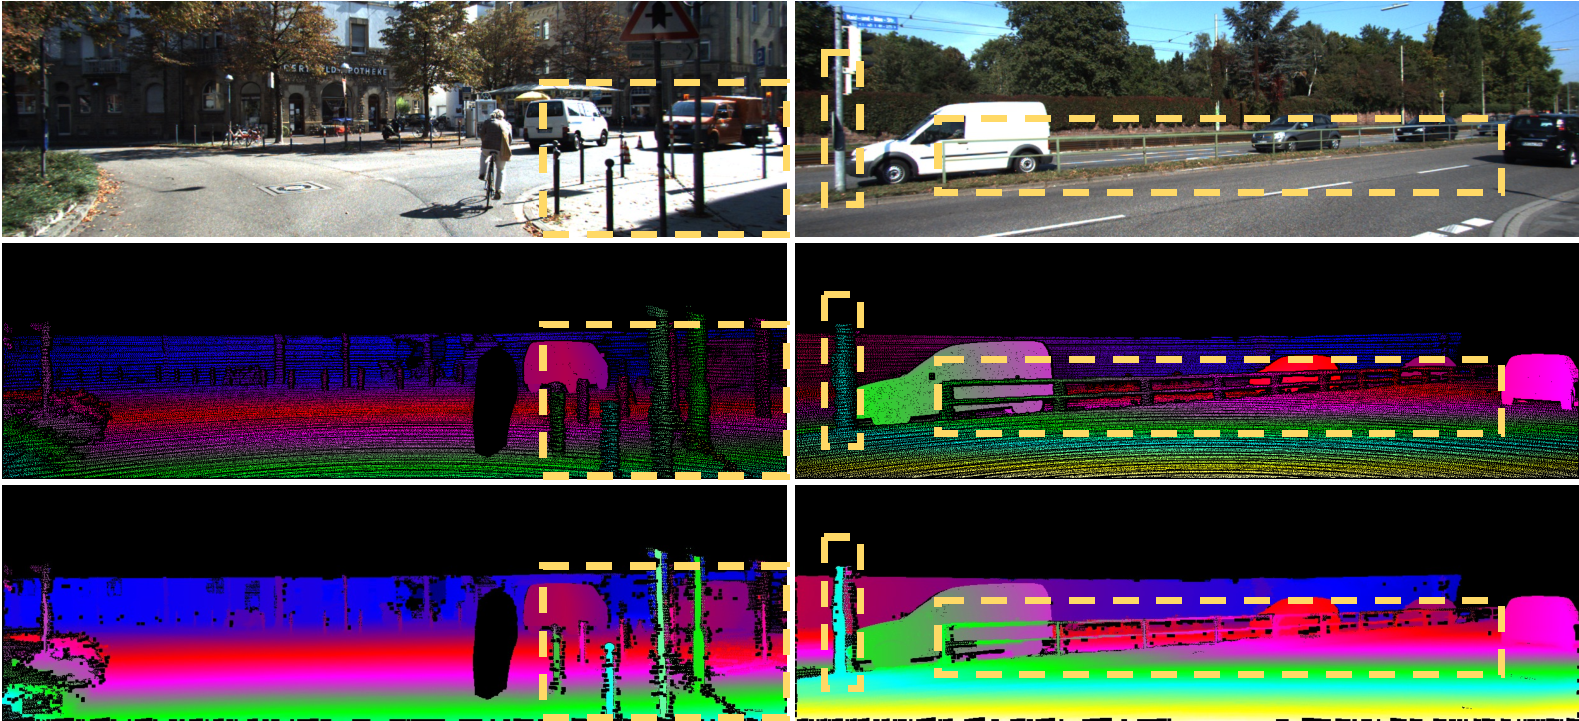
\includegraphics[width=0.99\linewidth]{fig/pseudo/pseudo.pdf}
	\vspace{-0.5em}
	\caption{
	\textbf{Depth Labels in KITTI.} First row: reference images, middle row: sparse ground-truth depth labels,
	last row: pseudo depth labels generated by our approach. Notably, ground truth depth labels suffer from thickening issues and our method restores the fine-grained structures from noisy ground truth labels. Black regions are ignored during training.
	}
	\label{fig:pseudo-labels}
	\vspace{-1.2em}
\end{figure}

\section{Experiments}

\subsection{Controlled Evaluation on KITTI-CARLA}

Evaluating pseudo-label quality on real-world datasets like KITTI is difficult because dense ground-truth disparities are not available for the benchmark test set, and the training labels are sparse and noisy.
Instead, we curate a synthetic datasets using KITTI-CARLA~\cite{deschaud2021kitticarla} to emulate KITTI's sparse and noisy depth annotations.
Following KITTI's data collection protocol, LiDAR points are integrated over a temporal window of 21 frames (spanning $[-10, +10]$ frames relative to the current frame) to generate sparse depth maps.
To simulate real-world measurement noise, perturbations are applied to LiDAR points and sensor poses during integration: Gaussian noise ($\sigma=1.5\,\mathrm{cm}$) is added to LiDAR points, while poses are perturbed with translational ($\sigma=2\,\mathrm{cm}$) and rotational ($\sigma=0.07^\circ$) random noise.
This procedure ensures depth maps exhibit sparsity and noise characteristics consistent with KITTI's ground truth.
The curated dataset is divided into 24,500 training and 10,500 test image pairs.
Sparse and noisy disparity maps are used for training and pseudo-label generation, while the precise KITTI-CARLA ground-truth disparities are reserved for evaluation.

Using the curated KITTI-CARLA dataset, we conduct a controlled experiment.
We compare two training strategies using the same NMRF architecture and hyperparameters.
The baseline model is trained directly with the sparse noisy labels.
The proposed model is trained with additional pseudo labels generated by structure-aware depth completion.
As shown in Table~\ref{tab:pseudo} (right), our additional pseudo labels bring a 32.3\% reduction in End-Point Error (EPE) and a 15.9\% improvement in the D1 metric (percentage of erroneous pixels with disparity error larger than 3 pixels and 5\% of the ground truth).
Qualitative results (Figure~\ref{fig:res_thin}) further demonstrate that pseudo-labels suppress the ``thickening'' artifacts, \ie, erroneous depth discontinuities induced by noisy supervision, yielding sharper object boundaries aligned with the reference image.
These results underscore the capability of pseudo labels to mitigate the label noise, enabling the model to achieve robust performance under imperfect real-world conditions.

Beyond disparity estimation, we evaluate the impact of pseudo label generation on surface normal quality, critical output for downstream 3D tasks (\eg, mesh reconstruction), obviating the need for an additional dedicated normal estimation network.
Surface normals are derived directly from disparity maps using camera intrinsic parameters, as described in~\cite{rossi2020joint}.
To isolate the effect of auxiliary loss (Equation~\ref{eq:loss-aux}), we train original NMRF and our adapted version on the SceneFlow dataset and evaluate normal errors on its test set.
Normal accuracy is quantified as the percentage of pixels with angular errors exceeding thresholds $t\in \{10^\circ,15^\circ,20^\circ,30^\circ\}$ (lower is better).
As reported in Table~\ref{tab:pseudo}, our auxiliary supervision reduces the error rate under the $20^\circ$ threshold by 35.6\%, confirming that our auxiliary supervision grounded on energy-based optimization enforces geometric consistency crucial for accurate normal derivation.
This highlights the broader utility of neural-energy fusion in learning geometrically coherent representation for robotic perception.
\begin{table}[t!]
	\centering
	\footnotesize
	\caption{Left: surface normal evaluation on the SceneFlow~\cite{mayer2016large}, where normal maps are derived from disparity estimates using the approach in~\cite{rossi2020joint}. Right: disparity evaluation on curated KITTI-CARLA dataset~\cite{deschaud2021kitticarla}. Bold values indicate the better performance for each metric.}
	\resizebox{0.99\linewidth}{!}{
		%\setlength\tabcolsep{2pt}
		\renewcommand\arraystretch{1.05}
		\begin{tabular}{l|cccc|cccc}
			\toprule
			\multirow[c]{2}{*}{Methods}
			& \multicolumn{4}{c|}{SceneFlow~\cite{mayer2016large}}
			& \multicolumn{4}{c}{Curated KITTI-CARLA~\cite{deschaud2021kitticarla}}\\
			%\cmidrule{2-9}
			\cline{2-9}
			& {\scriptsize $10^\circ$} & {\scriptsize $15^\circ$} & {\scriptsize $20^\circ$} & {\scriptsize $30^\circ$}
			& EPE & D1 & bad 1 & bad 3\\
			\midrule
			NMRF~\cite{guan2024neural} & 55.33 & 43.20 & 34.91 & 24.18 & 0.96 & 4.98 & 6.95 & 5.07\\
			Ours & \textbf{38.92} & \textbf{28.92} & \textbf{22.49} & \textbf{14.83} & \textbf{0.65} & \textbf{4.19} & \textbf{6.53} & \textbf{4.35}\\
			\bottomrule
		\end{tabular}
	}
	\label{tab:pseudo}
\end{table}

\begin{figure}[!t]
	\centering
	\tabcolsep=0.03cm
	\begin{tabular}{c c}
		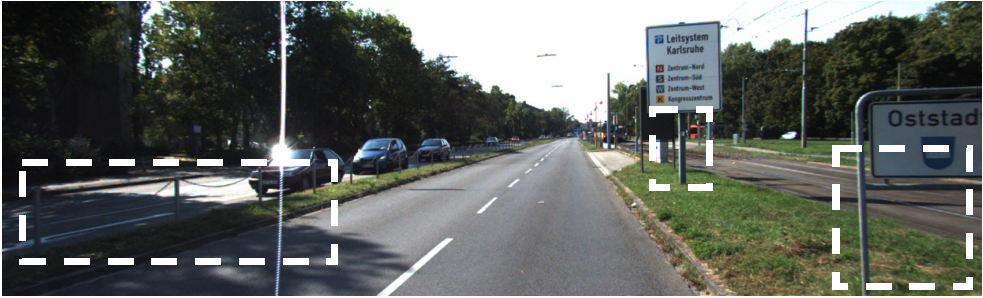
\includegraphics[width=0.49\linewidth]{fig/pseudo/thin_rgb.pdf}& 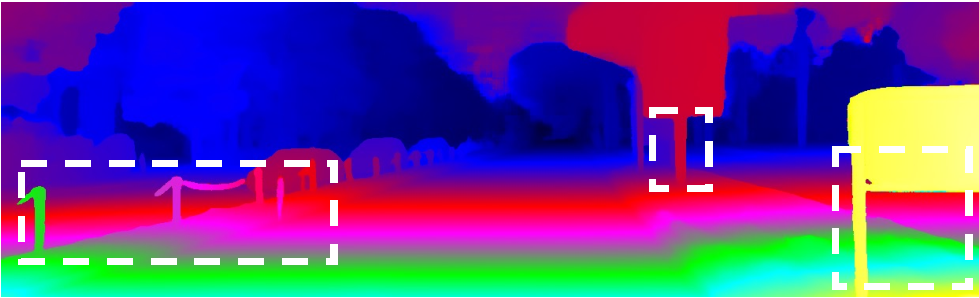
\includegraphics[width=0.49\linewidth]{fig/pseudo/thin_nmrf.pdf}\vspace{-1.0mm}\\ 
		(a) \textsf{\footnotesize Reference image} & (b) \textsf{\footnotesize NMRF~\cite{guan2024neural}}\\ 
		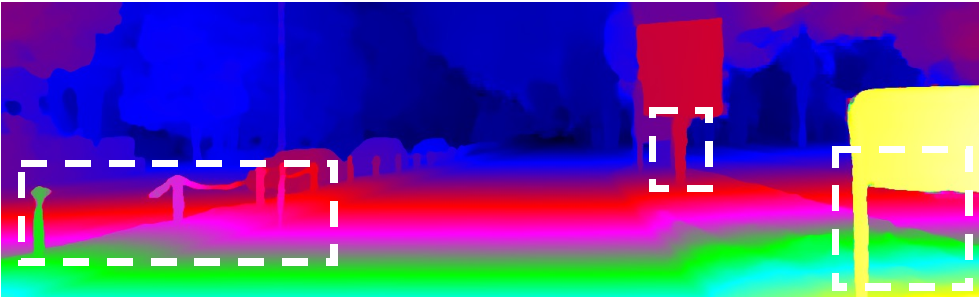
\includegraphics[width=0.49\linewidth]{fig/pseudo/thin_igev.pdf}& 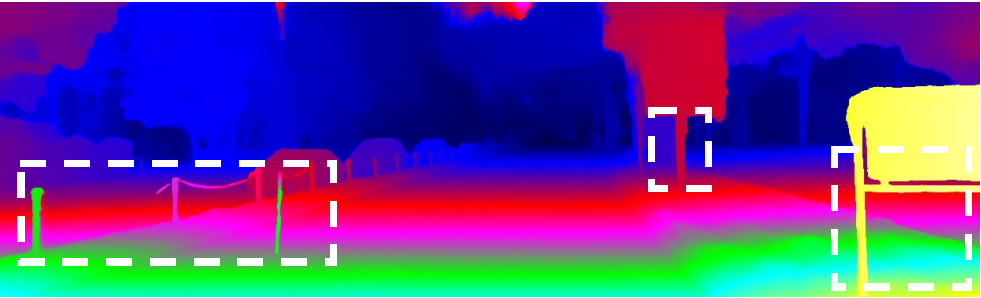
\includegraphics[width=0.49\linewidth]{fig/pseudo/thin_ours.pdf}\vspace{-1.0mm}\\
		(c) \textsf{\footnotesize IGEV~\cite{xu2023iterative}} & (d) \textsf{\footnotesize Ours}
	\end{tabular}
	%\vspace{-0.8em}
	\caption{\textbf{Qualitative results on KITTI benchmark.} Noisy ground truth depth labels lead to overly thickening object boundaries, even in state-of-the-art models~\cite{guan2024neural,xu2023iterative}. Our pseudo label supervision approach effectively mitigates this issue, preserving thin structures and holes.}
	\label{fig:res_thin}
	\vspace{-1.2em}
\end{figure}

\chapter{Bridging Monocular and Stereo Reasoning with Latent Alignment}\label{ch:bridgedepth}
\section{Introduction}
Chapter~\ref{ch:nmrf} and~\ref{ch:pseudo-label} introduced neural Markov random fields for stereo matching, a framework that recasts classical graphical-model inference as a learnable message-passing network.
The key advantage of this formulation is that it preserves an important geometric inductive bias of stereo vision: depth is inferred by selecting, propagating, and refining disparity hypotheses under local spatial consistency constraints.
By combing disparity proposal generation, neural message passing, and learned regularization, the resulting model achieves accurate and efficient stereo matching while retaining the interpretability of hypothesis-based correspondence reasoning.
Nevertheless, the approach remains fundamentally stereo-centric.
Its evidence comes primarily from correspondences between two views, and it therefore inherits a central limitation of stereo matching: when image correspondence becomes unreliable, the recovered geometry may also become unstable as well.

This limitation is closely connected to the broader motivation of this thesis.
Robust visual geometry is difficult to recover from a single source of evidence.
Stereo correspondence provides metric constraints through epipolar geometry and is highly effective when reliable matches are available.
Yet stereo reasoning is fragile in regions where matching is ambiguous or misleading, including weakly textured surfaces, repetitive patterns, occlusions, transparent materials, and specular reflections.
These failures are not merely artifacts of a particular network architecture.
They reveal an intrinsic weakness of correspondence-based geometry: when the image evidence does not uniquely identify the correct match, local matching alone cannot provide a stable geometric explanation.

Monocular perception provides a complementary form of evidence.
Although a single image cannot uniquely determine metric 3D structure, it contains rich contextual cues, including semantic layout, object-level regularities, perspective, surface continuity, and learned priors about scene organization.
Recent large-scale monocular foundation models~\cite{ranftl2020towards,ke2023repurposing,depth_anything_v1,piccinelli2024unidepth} have substantially strengthened this form of holistic depth reasoning, producing coherent depth ordering and plausible scene  structures across diverse visual domains.
Such models can be more robust than stereo matching in regions where local correspondence is ambiguous, because they can infer structure from global context rather than relying only on pixel-level matching evidence.
At the same time, monocular depth remains geometrically under-constrained.
Without explicit multi-view constraints, monocular predictions may lack metric accuracy, fine local details, and reliable scale.

The natural step beyond neural MRF stereo matching is therefore not to abandon correspondence reasoning, but to enrich it with monocular context while preserving the metric precision of stereo geometry.
This chapter explores that direction by studying how monocular and stereo representations can be unified during geometrical reasoning.
The central observation is that their strengths are complementary at the level of latent representation.
Monocular features provide structural priors that can regularize ambiguous disparity hypotheses, while stereo hypotheses provide metric geometric evidence that can ground monocular depth reasoning.
A unified model should therefore allow these two forms of reasoning to interact before the final prediction is made, rather than combining their outputs only after separate reasoning processes have already been completed.

To this end, this chapter presents \emph{BridgeDepth}, a latent alignment approach that integrates monocular contextual reasoning and stereo geometric matching within a single network.
Instead of treating monocular depth as an external prior, an auxiliary prediction, or a post-hoc fusion signal, BridgeDepth introduces monocular contextual representations directly into the stereo hypothesis aggregation.
The monocular branch extracts structural features from a pretrained depth foundation model, while the stereo branch maintains a compact set of disparity hypotheses at each pixel.
To make cross-modal interaction efficient, the stereo search space is first pruned into a small number of representative hypotheses, following the proposal-based reasoning introduced in NMRF~\cite{guan2024neural}.
This compact hypothesis representation provides a tractable interface for aligning monocular context with stereo geometry.

The core of BridgeDepth is an iterative bidirectional latent alignment mechanism.
At each alignment step, stereo hypotheses first perform a \emph{monocular-readout} operation, in which they attend to monocular contextual features through cross-attention.
This operation allows semantic and structural priors to guide correspondence reasoning before stereo cost aggregation, especially in ambiguous regions where local matching evidence is weak or deceptive.
The stereo hypotheses are then aggregated through neural message passing, which propagates geometric consistency across neighboring pixels and resolves competition among candidate disparities.
After aggregation, a reverse \emph{monocular-update} operation lets monocular features attend back to the refined stereo hypotheses.
In this direction, geometrically validated correspondence information is injected into the monocular representation, reducing its ambiguity and improving its consistency with metric scene structure.
Through iterative readout, aggregation, and update operations, monocular context and stereo geometry are progressively synchronized in a shared latent space.

This bidirectional alignment design is important for the thesis narrative because it moves beyond treating visual geometry as a collection of isolated estimation problems.
The previous chapters showed that stereo matching benefits from structured hypothesis reasoning, where disparity candidates are refined through learned message passing under spatial consistency.
However, the source of geometric evidence in that formulation is still largely restricted to binocular correspondence.
BridgeDepth extends this reasoning paradigm by introducing monocular scene understanding into the hypothesis aggregation process.
Each disparity hypothesis is therefore evaluated not only by local matching evidence, but also by contextual priors about scene layout, object structure, and surface continuity.
At the same time, the monocular representation is updated by aggregated stereo hypotheses, so its contextual features become grounded by metric geometric constraints rather than remaining purely prior-driven.

This mechanism is more than a fusion strategy for improving stereo depth estimation.
It represents a step forward the broader goal of this thesis: learning unified geometric representations in which complementary visual cues interact during reasoning.
Rather than concatenating monocular and stereo features or applying a final-stage correction to the stereo output, BridgeDepth establishes a recurrent exchange between contextual priors and geometric evidence.
Through this exchange, monocular reasoning becomes more geometrically constrained, while stereo reasoning becomes more robust to ambiguous correspondence.
The resulting formulation reflects the central hypothesis of this thesis: robust structure and motion estimation requires a coherent latent space in which multiple sources of visual geometry, including spatial correspondence, semantic context, and eventually temporal motion cues, can be jointly represented and refined.

Following this principle, BridgeDepth preserves separate task-specific predictions while allowing their underlying representations to interact.
The framework produces two outputs: a metric disparity map from the stereo stream and a relative depth map from the monocular stream.
The stereo output remains the primary source of geometrically accurate reconstruction, as it is directly constrained by binocular correspondences.
The monocular output, however, is not merely an auxiliary prediction used for additional supervision.
Since the monocular representation is repeatedly updated by aggregated stereo hypotheses, its prediction indicates whether metric geometric evidence has been successfully injected into the contextual stream.
The dual-output design therefore encourages bidirectional alignment during training and provides a direct way to examine its effect: stereo reasoning becomes more robust through monocular priors, while monocular reasoning becomes more consistent with multi-view geometry.

The effectiveness of this design is validated through extensive experiments.
On standard stereo benchmarks, BridgeDepth achieves competitive or state-of-the-art accuracy while maintaining efficient inference.
More importantly, it substantially improves zero-shot generalization from synthetic training data to real-world datasets such as Middlebury and ETH3D, where domain shift and correspondence ambiguity are particularly challenging.
Qualitative results in Figure~\ref{fig:tsear}, further show stronger robustness on reflective and transparent surfaces, where conventional stereo methods often produce fragmented or physically implausible disparities.
These results support the central argument of this chapter: monocular context and stereo geometry should not be treated as independent estimators whose outputs are fused after separate prediction, but as complementary representations that are aligned and refined during latent reasoning.

\begin{figure}[!t]
	\centering
	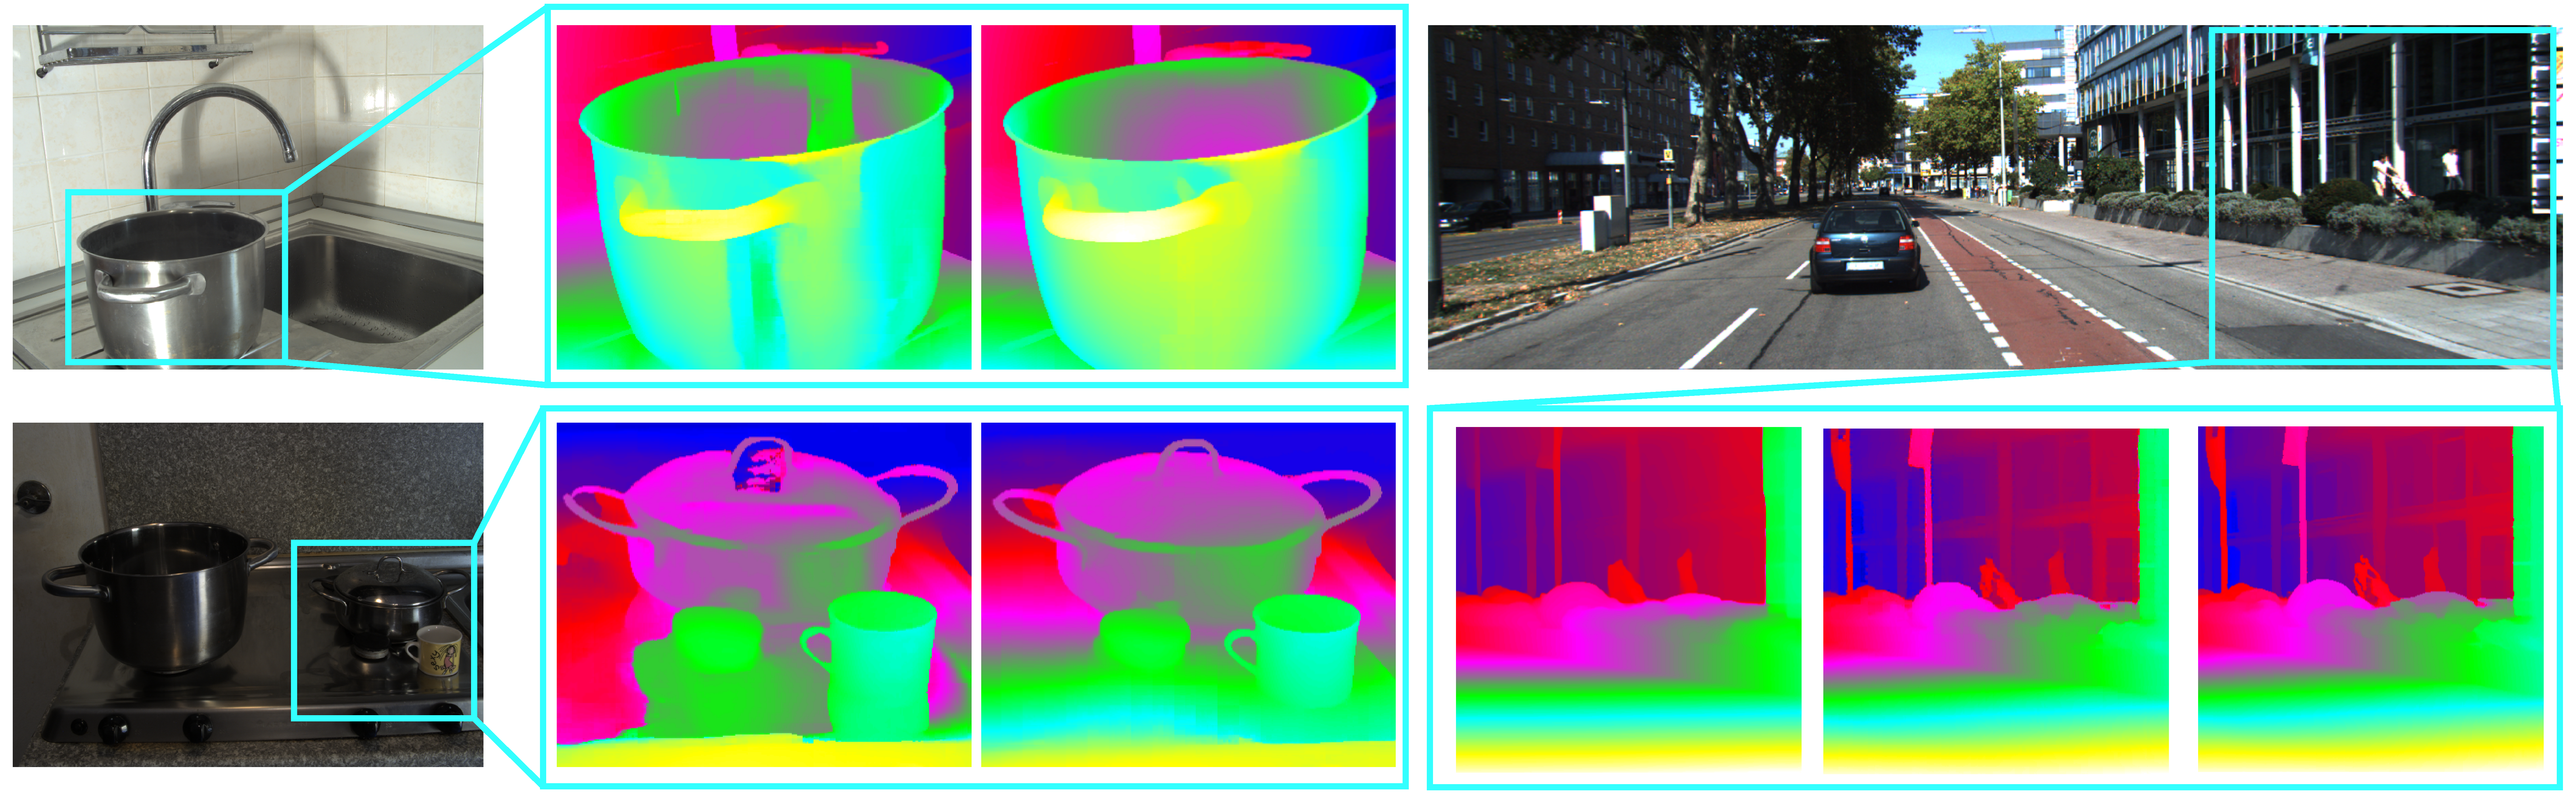
\includegraphics[width=0.99\linewidth]{fig/bridgedepth/bridgedepth.pdf}\\
	\makebox[0.21\linewidth]{}
	\makebox[0.16\linewidth]{\footnotesize \textsf{NMRF~\cite{guan2024neural}}}
	\makebox[0.17\linewidth]{\footnotesize \hspace{-0.5em}\textsf{Ours-\emph{Stereo}}}
	\makebox[0.14\linewidth]{\footnotesize \textsf{DepthAnythingV2~\cite{yang2024depth}}}
	\makebox[0.14\linewidth]{\footnotesize \textsf{Ours-\emph{Mono}}}
	\makebox[0.14\linewidth]{\footnotesize \textsf{Ours-\emph{Stereo}}}
	\vspace{-5pt}
	\captionof{figure}{By aligning latent representations, the proposed approach unifies monocular geometric reasoning with stereo matching.
	It achieves both higher overall depth accuracy and finer detail than the monocular baseline DepthAnythingV2~\cite{yang2024depth}, while also improving over the stereo method NMRF~\cite{guan2024neural}, particularly on textureless surfaces and reflective regions where correspondence is unreliable.}
	\label{fig:tsear}
	\vspace{-5pt}
\end{figure}

In summary, this chapter extends the hypothesis-based stereo architecture developed in Chapter~\ref{ch:nmrf} into a unified monocular and stereo reasoning formulation.
The proposed method preserves the metric precision of stereo matching while incorporating the robustness of monocular contextual reasoning.
By aligning spatial correspondence and semantic context within a shared representation, BridgeDepth provides a concrete instance of the broader thesis hypothesis: robust visual geometry emerges when complementary cues jointly shape the reasoning process rather than acting in isolation.

\section{Methodology}
\subsection{Overview of the Architecture}
Given a rectified stereo pair $\bm{I}_1, \bm{I}_2$, the approach estimates two outputs: a metric disparity map $D$ from the stereo reasoning stream and a relative depth map $R$ from the monocular reasoning stream.
The architecture consists of two stages, as illustrated in Figure~\ref{fig:bridgedepth_overview}.
The first stage, \textbf{pre-alignment}, constructs modality-specific representations.
The monocular stream processes the reference image $\bm{I}_1$ using a pretrained monocular depth foundation model and extracts a contextual feature map.
The stereo stream extracts multi-scale features from both images and uses a Disparity Proposal Network (DPN) to produce a small set of candidate disparities at each pixel.
Each candidate is then embedded as a latent stereo hypothesis.
The second stage, \textbf{bidirectional latent alignment}, iteratively synchronizes the monocular and stereo representations.
At each alignment step, stereo hypotheses first read from monocular features through cross-attention.
This readout injects contextual priors into the stereo hypotheses before cost aggregation.
The stereo hypotheses are then aggregated using neural message passing, which performs both inter-pixel propagation and intra-pixel hypothesis competition.
Finally, the monocular features are updated by attending to the aggregated stereo hypotheses, allowing geometrically validated information to flow back into the monocular stream.
A coarse-to-fine cascade further refines disparity at a higher spatial resolution.

This design differs from post-hoc fusion~\cite{bae2022multi,li2024local} in an important way. 
The monocular and stereo streams are not merely combined near the output.
Instead, they interact throughout the reasoning process, allowing the model to learn a shared latent space in which monocular context and stereo geometry mutually constrain each other.

\begin{figure}[!t]
	\centering
	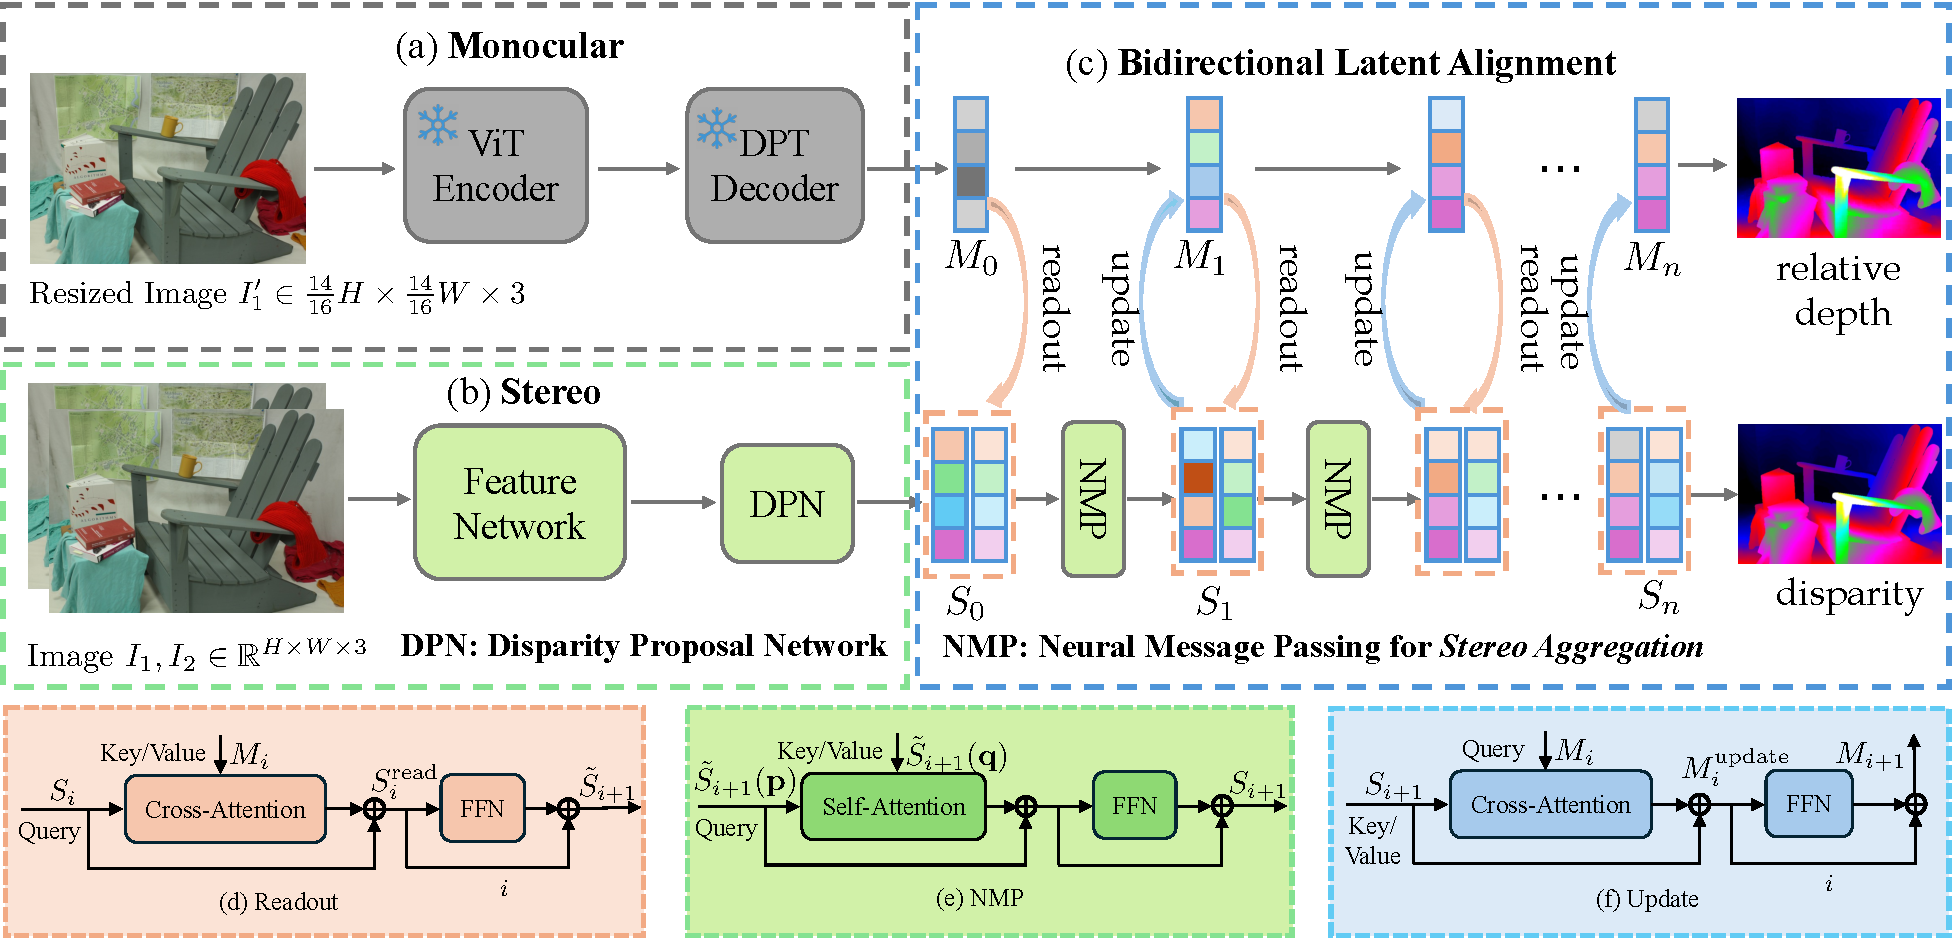
\includegraphics[width=0.97\linewidth]{fig/bridgedepth/bridgedepth_overview.pdf}
	\caption{\textbf{Architecture of the proposed BridgeDepth framework.} The model operates in two phases.
	During pre-alignment, (a) a monocular encoder aggregates contextual information from the reference view, while (b) a stereo pathway uses DPN~\cite{guan2024neural} to reduce the disparity search space from 40 labels to 2 candidate labels. 
	During bidirectional latent alignment, (c) the two modalities are iteratively synchronized through cross-modal interaction; spatial dimensions are collapsed in the diagram for clarity. 
	The network predicts relative depth from the monocular stream and metric disparity from the stereo stream.}
	\label{fig:bridgedepth_overview}
	\vspace{-0.8em}
\end{figure}

\subsection{Monocular Contextual Feature Extraction}
The monocular stream is initialized from a pretrained monocular depth foundation model.
In the implementation described in this chapter, the stream follows a  DepthAnything-style architecture that combines a DINOv2~\cite{oquab2023dinov2} visual encoder with a DPT~\cite{ranftl2021vision} decoder.
The pretrained encoder provides strong general-purpose visual features, while the decoder aggregates multi-level representations into dense contextual features for depth prediction.
Let $\bm{I}_1 \in \mathbb{R}^{H \times W \times 3}$ denote the reference image.
To match the $14\times 14$ patch size of the ViT encoder, the image is resized by a factor of $14/16$, producing $\bm{I}_1'$.
The DPT decoder outputs a feature map whose spatial resolution corresponds to $8/14$ of $\bm{I}_1'$, \ie one half of the original image resolution.
This feature map is then downsampled by a strided-4 convolution so that its resolution matches the coarse stereo branch.
The resulting monocular feature map is denoted as
$M_0 \in \mathbb{R}^{\frac{H}{8} \times \frac{W}{8} \times C}$.
The role of $M_0$ is not limited to monocular depth prediction. 
It serves as a contextual memory that encodes semantic layout, object structure, surface continuity, and monocular depth priors. 
These cues are later queried by stereo hypotheses during alignment.
In the main configuration, the pretrained monocular stream is frozen during training.
Freezing helps preserve the generalization capability learned from internet-scale data and prevents the stereo training set from over-specializing the monocular representation.
Additional experiments (see Table~\ref{tab:mono_foundation}) show that the framework is compatible with multiple monocular backbones, including diffferent variants of DepthAnythingV2~\cite{yang2024depth}, UniDepthV2~\cite{piccinelli2025unidepthv2}, and MoGe~\cite{wang2025moge,wang2025moge2} models.

\subsection{Stereo Hypothesis Representation}
\noindent\textbf{Multi-scale stereo feature extraction.}
The stereo stream extracts image features from the left and right views using a Siamese feature network.
For each scale $s \in \{4,8\}$, the network produces feature maps $\bm{F}_{1,s}, \bm{F}_{2,s} \in \mathbb{R}^{\frac{H}{s} \times \frac{W}{s} \times C}$, where $\bm{F}_{1,s}$ and $\bm{F}_{2,s}$ correspond to the reference and target images, respectively.
The $1/8$-resolution features are used for coarse stereo reasoning, while the $1/4$-resolution features are later used for fine-grained refinement.

A conventional cost-volume formulation would evaluate many disparity candidates at each pixel.
For example, if the maximum disparity is 320 pixels and the feature stride is 8, the coarse disparity dimension contains approximately 40 candidates.
Directly aligning such a dense cost volume with monocular features would be computationally expensive because cross-attention complexity grows quadratically with both the number of spatial tokens and the number of disparity hypotheses.

\noindent\textbf{Disparity hypotheses pruning.}
To make cross-modal alignment efficient, the stereo stream uses a disparity proposal mechanism to reduce the number of hypotheses.
Starting from the coarse feature maps $\bm{F}_{1,8}$ and $\bm{F}_{2,8}$, the proposal module computes matching scores over the initial disparity range and selects the top $K$ candidates for each pixel. 
In the default configuration, the full candidate set is reduced from 40 to $K=2$ hypotheses per pixel.
A disparity propagation module~\cite{guan2024neural} then refines the selected candidates by spreading plausible disparities over local neighborhoods and suppressing unlikely ones.
The resulting candidates are denoted by $\{d^k_{i,j}\}_{k=1}^{K}$,
where $d^k_{i,j}$ is the $k$-th disparity proposal at pixel $(i,j)$ on the coarse grid.
This compact representation preserves the main disparity modes while making bidirectional alignment tractable.

\noindent\textbf{Hypothesis embedding.}
Each disparity candidate is embedded into a latent vector that combines concatenation-based and correlation-based matching cues. For the $k$-th hypothesis at location $(i,j)$, the embedding is defined as
\begin{align}
	S_0(i,j,k)&=\text{FFN}\left(\mathbf{x}_{i,j,k}^{{\tt concat}} \parallel \mathbf{x}_{i,j,k}^{{\tt corr}}\right), \nonumber \\
	\mathbf{x}_{i,j,k}^{{\tt concat}}&=\delta_1\left(\bm{F}_{1,8}(i,j)\right) \parallel\delta_1\left(\bm{F}_{2,8}(i,j-d_{i,j}^{k})\right), \label{eq:hypothesis-embedding} \\
	\mathbf{x}_{i,j,k}^{{\tt corr}}(g)&=\frac{G}{C}\left\langle\delta_2(\bm{F}_{1,8}(i,j,g)),\delta_2(\bm{F}_{2,8}(i,j-d_{i,j}^k,g))\right\rangle \nonumber.
\end{align}
Here, $\parallel$ denotes channel concatenation.
The feature channels are divided into $G$ groups for grouped correlation, and $g$ indexes one group.
The functions $\delta_1$ and $\delta_2$ normalize the feature distributions before concatenation and correlation. 
Each consists of convolutional layers with normalization and nonlinear activation. 
For sub-pixel disparity proposals, bilinear sampling is used to obtain the right-image feature at the shifted location.
The embedded stereo hypotheses are collected as
$S_0 \in \mathbb{R}^{\frac{H}{8} \times \frac{W}{8} \times K \times C}$.
This tensor is the stereo counterpart of the monocular contextual features $M_0$ and serves as the input to the latent alignment module.

\subsection{Bidirectional Latent Alignment}
The bidirectional alignment module performs iterative interaction between monocular contextual features and stereo hypothesis embeddings.
Let $M_i$ and $S_i$ denote the monocular and stereo representations at iteration $i$.
Each iteration contains three operations: monocular readout, stereo aggregation, and monocular update.

\noindent\textbf{Monocular readout: context-guided stereo hypotheses.}
Before stereo aggregation, the stereo hypotheses query the monocular feature map, as illustrated in Figure~\ref{fig:bridgedepth_overview} (d).
This operation allows each disparity hypothesis to access contextual information such as object boundaries, semantic regions, and likely structure layout.
For efficiency, the feature maps are divided into non-overlapping $N\times N$ spatial windows.
Within each window, the stereo embeddings serve as queries, while the monocular features serves as key and values:
\begin{equation} \begin{aligned} Q_s = \mathrm{LN}(S_i) W_q, \quad K_m = \mathrm{LN}(M_i) W_k, \quad V_m = \mathrm{LN}(M_i) W_v. \end{aligned} \end{equation}
The readout operation is then defined as
\begin{align} 
	S_i^{\mathrm{read}} &= S_i + \mathrm{WindowAttn}(Q_s, K_m, V_m), \\ \widetilde{S}_{i+1} &= S_i^{\mathrm{read}} + \mathrm{FFN}\left(\mathrm{LN}(S_i^{\mathrm{read}})\right). 
	\label{eq:bridge_readout}
\end{align}
This produces contextual-aware stereo embeddings $\widetilde{S}_{i+1}$, which are subsequently aggregated by the stereo reasoning module.

\noindent\textbf{Content-adaptive positional bias.} The window attention in Equation~\ref{eq:bridge_readout} adopts a content-adaptive positional bias to preserve spatial structure during cross-modal interaction.
For query, key, and value tensors $Q$, $K$, and $V$, attention is computed as
\begin{equation} \mathrm{WindowAttn}(Q,K,V) = \mathrm{softmax}\left(\frac{QK^{\top}}{\sqrt{d}} + \beta \right)V, \end{equation}
with
\begin{equation} \beta = Q^{\top}R^k + K^{\top}R^q. \label{eq:bridge_pos_bias} \end{equation}
The learnable position embeddings $R^q$ and $R^k$ encode relative positions inside a window and distinguish the roles of query and key tokens.
Unlike a fixed relative bias, this formulation lets the positional term depend on feature content, allowing the attention mechanism to adapt spatial aggregation according to local image structure.

\noindent\textbf{Stereo aggregation by neural message passing.} After monocular readout, the stereo hypotheses are aggregated using neural message passing (NMP) module of NMRF, as depicted in Figure~\ref{fig:bridgedepth_overview} (e).
This module can be interpreted as a structured form of self-attention over the stereo hypothesis graph.
It performs two complementary operations.
First, inter-pixel aggregation propagates information between neighboring pixels.
This encourages adjacent pixels on the same surface to support consistent disparity hypotheses while still allowing discontinuities near object boundaries.
Second, intra-pixel aggregation models competition among multiple hypotheses at the same pixel.
This helps suppress inconsistent candidates and sharpen the posterior around the most plausible disparity.
The output of this aggregation step is denoted as
\begin{equation} S_{i+1} = \mathrm{NMP}\left(\widetilde{S}_{i+1}\right), \end{equation}
where $S_{i+1}$ contains stereo hypotheses that have been refined using both monocular contextual priors and geometric consistency from neighboring hypotheses.

\noindent\textbf{Monocular update: geometry-grounded contextual features.}
The second direction of alignment, shown in Figure~\ref{fig:bridgedepth_overview} (f), injects stereo-validated geometric information back into the monocular stream.
After stereo aggregation, the monocular features query the updated stereo embeddings:
\begin{equation} \begin{aligned} Q_m = \mathrm{LN}(M_i) W'q, \quad K_s = \mathrm{LN}(S_{i+1}) W'k, \quad V_s = \mathrm{LN}(S_{i+1}) W'_v. \end{aligned} \end{equation}
The monocular update is given by
\begin{align} 
	M_i^{\mathrm{update}} &= M_i + \mathrm{WindowAttn}(Q_m, K_s, V_s), \\
	 M_{i+1} &= M_i^{\mathrm{update}} + \mathrm{FFN}\left(\mathrm{LN}(M_i^{\mathrm{update}})\right).
	\label{eq:bridge_update} 
\end{align}
This operation grounds the monocular features with geometric evidence, including disparity boundaries, depth ordering, and local surface consistency.
The updated contextual representation is therefore no longer purely monocular; it becomes a geometry-aware latent representation refined by stereo geometry evidence.

\noindent\textbf{Iterative alignment.} The readout, aggregation, and update operations form one alignment block.
Stacking multiple blocks creates an iterative refinement process:
\begin{equation} (M_i, S_i) \rightarrow (M_{i+1}, S_{i+1}), \quad i=0,\ldots,l-1. \end{equation}
Each iteration improves the consistency between monocular and stereo representations.
Stereo hypotheses become more aware of global scene structure, while monocular features become more geometrically grounded.
This iterative exchange is the core difference between latent alignment and static feature fusion.

\subsection{Coarse-to-Fine Detail Recovery}
The main alignment stage operates at $1/8$ of input image resolution for efficiency.
Although this resolution is sufficient for robust global reasoning, it may miss thin structures and sharp disparity discontinuities.
To recover fine details, the model uses a coarse-to-fine refinement stage.
After $l$ iterations of coarse alignment, the stereo stream decodes a coarse disparity prediction $D_{\mathrm{coarse}}$. 
This disparity is downsampled to the $1/4$ scale using median pooling, which preserves discontinuities better than average pooling.
The downsampled disparity initializes a new set of fine-level stereo embeddings using the $1/4$-resolution image features $\bm{F}_{1,4}$ and $\bm{F}_{2,4}$.
The same feature-warping and grouped-correlation formulation used to construct $S_0$ is applied at this higher resolution.

To balance accuracy and efficiency, the stereo stream is refined at $1/4$ resolution while the monocular stream remains at $1/8$ resolution.
Since the two streams now have different spatial scales, the cross-attention window size of the monocular stream is adjusted so that windows in both stream cover an equivalent image region.
In practice, if the stereo window size is $N$, the monocular window size is reduced to $N/2$.
This asymmetric design allows the framework to recover fine geometric structures without running full monocular-stereo alignment at high resolution.
The fine-level stereo embeddings continue to query monocular context and update the monocular representation, while the computational cost remains manageable.

\subsection{Dual Output Prediction}
After the coarse and fine alignment stages, the model decodes two outputs: metric disparity from the stereo stream and relative depth from the monocular stream.
The stereo decoder maps the final stereo embeddings to a full-resolution disparity map.
A lightweight multilayer perceptron projects the $1/4$-resolution embeddings into a feature tensor with 16 channels for spatial reconstruction. 
A pixel shuffle operation then produces the full-resolution disparity map $D \in \mathbb{R}^{H \times W}$.
The monocular decoder follows an analogous structure and predicts a relative depth map $R \in \mathbb{R}^{H \times W}$.

The dual-output design has two purposes.
First, it provides direct supervision to both streams and encourages the monocular representation to participate in the alignment process.
Second, it offers a diagnostic signal for whether stereo geometry has been transferred back to the monocular stream.
If the monocular output becomes more scale-consistent and detail-preserving after alignment, this indicates that the monocular features have absorbed useful geometric information rather than merely acting as a static prior for stereo matching.
More broadly, this dual-output strategy suggests a general pattern for multi-cue visual geometry.
When two cues are complementary, the network can learn not only to produce one final estimate but also to maintain task-specific outputs that regularize the shared latent representation.
This idea is relevant beyond stereo vision, for example to the joint modeling of depth and optical flow, where monocular depth and temporal correspondence could be aligned in a similar way.

\subsection{Training Objective}
The framework is trained with stereo and monocular losses.
Let $\{D_i\}_{i=0}^{l+l^{\prime}-1}$ denote the sequence of disparity predictions from all alignment iterations, with $l$ coarse resolution iterations and $l^{\prime}$ fine-resolution iterations.
Similarly, let $\{R_i\}_{i=0}^{l+l^{\prime}-1}$ denote the corresponding monocular relative depth predictions.
The stereo stream is supervised with an $L1$ disparity loss:
\begin{equation} \mathcal{L}_{\mathrm{stereo}} = \sum_{i=0}^{l+l^{\prime}-1} w_i \left|D_i - D_{\mathrm{gt}}\right|_1, \label{eq:bridge_stereo_loss} 
\end{equation}
where $D_{\mathrm{gt}}$ is the ground-truth disparity and $w_i$ balances predictions from different iterations.
The monocular stream is supervised using an affine-invariant loss:
\begin{equation} \mathcal{L}_{\mathrm{mono}} = \sum_{i=0}^{l+l^{\prime}-1} \gamma^{l+l^{\prime}-i} \rho\left(R_i, D_{\mathrm{gt}}\right), \label{eq:bridge_mono_loss} 
\end{equation}
where $\rho(\cdot,\cdot)$ denotes the affine-invariant depth loss introduced by MiDAS~\cite{ranftl2020towards}, and $\gamma=0.8$ controls the weighting over iterations.
Although the monocular branch predicts relative depth, the affine-invariant formulation allows it to be supervised using disparity-derived ground truth after accounting for scale and shift differences.

The final objective is
\begin{equation} 
\mathcal{L} = \mathcal{L}_{\mathrm{stereo}} + \lambda_{\mathrm{mono}}\mathcal{L}_{\mathrm{mono}}, 
\end{equation}
where $\lambda_{\mathrm{mono}}$ controls the strength of monocular supervision.
In practice, the monocular loss improves generalization because it explicitly enforces consistency between the contextual representation and metric stereo geometry.

\subsection{Implementation Details}
The model is implemented in PyTorch and trained using the AdamW optimizer with a one-cycle learning-rate schedule.
Data augmentation follows common stereo training practice~\cite{guan2024neural,lipson2021raft}, including random cropping and appearance perturbation.
Unless otherwise stated, the monocular stream uses a frozen ViT-L version of the DepthAnythingV2~\cite{yang2024depth}.
The stereo feature extractor is based on a lightweight convolutional encoder.
Pretraining is performed on the Scene Flow dataset for 300K iterations with a batch size of 8.
Input images are randomly cropped to $384 \times 768$, and the learning rate follows a cosine one-cycle schedule with a peak value of $5\times10^{-4}$.
For KITTI evaluation, the Scene Flow pretrained model is further fine-tuned on mixed KITTI 2012 and KITTI 2015 training data for 40K iterations. 
Fine-tuning uses random crops of $304 \times 1152$, a batch size of 4, and a reduced peak learning rate of $2\times10^{-4}$.

An enlarged variant, BridgeDepth-L, replaces the lightweight ResNet stereo encoder with a stronger ConvNeXt-Tiny-based feature network~\cite{liu2022convnet}. 
The first three stages of the original ConvNext-Tiny backbone are adopted and produce features at $1/4$, $1/8$, and $1/16$ resolutions. 
A DPT-style fusion module merges these multi-scale features into a $1/4$-resolution representation with 128 channels, which is then average-pooled to obtain the $1/8$-resolution features used for coarse alignment. 
This variant demonstrates that the proposed alignment framework can benefit from stronger stereo features while preserving the same overall architecture.

\section{Experiments}
\subsection{Datasets and Metrics}
The model is evaluated on synthetic and real-world stereo benchmarks.
\textbf{Scene Flow}~\cite{mayer2016large} is used for synthetic pretraining and in-domain evaluation. 
It contains dense ground-truth disparity maps and includes FlyingThings3D, Driving, and Monkaa subsets.
\textbf{KITTI 2012}~\cite{geiger2012we} and \textbf{KITTI 2015}~\cite{menze2015object} are used for real-world driving scene evaluation.
They provide sparse LiDAR-based disparity annotations and are standard benchmarks for outdoor stereo matching.
\textbf{Middlebury 2014}~\cite{scharstein2014high} evaluates indoor stereo matching with high-resolution imagery and accurate structured-light ground truth.
It is used primarily for zero-shot generalization analysis.
\textbf{ETH3D}~\cite{schops2017multi} contains grayscale indoor and outdoor stereo pairs and provides another challenging zero-shot benchmark.
\textbf{Booster}~\cite{zamaramirez2022booster} is used for qualitative evaluation in ill-posed regions, especially reflective and transparent surfaces.

The experiments use the following standard disparity metrics.
\textbf{End-Point Error (EPE)} is the mean absolute disparity error over valid pixels.
\textbf{Bad-pixel rate (BP-$x$)} measures the percentage of pixels whose absolute disparity error exceeds $x$ pixels.
\textbf{D1 error} measures the percentage of pixels whose disparity error exceeds both an absolute threshold of 3 pixels and a relative threshold of $5\%$ of the ground-truth disparity.
For Scene Flow dataset, pixels with ground-truth disparity larger than 192 pixels are excluded following common evaluation protocol.

\subsection{Results}
\begin{table}[!t]
	\small
	\centering
	\resizebox{0.98\linewidth}{!}{
		\begin{tabular}{r c c c c c c c}
			\toprule 
			Method & RAFT-Stereo~\cite{lipson2021raft} & DLNR~\cite{zhao2023high} & 
			Selective-IGEV~\cite{wang2024selective} & NMRF~\cite{guan2024neural} & Mocha-Stereo~\cite{chen2024motif} & BridgeDepth & BridgeDepth-L\\
			\midrule
			EPE & 0.56 & 0.48 & 0.44 & 0.45 & 0.41 & 0.37 & \textbf{0.32}\\
			BP-1 &6.63 &5.39&4.98&4.50&5.07&3.67&\textbf{3.25}\\
			\bottomrule
		\end{tabular}
	}
	\vspace{-0.5em}
	\caption{\textbf{Performance on the Scene Flow test split.} Across both error metrics, the proposed method outperforms all prior stereo models. \textbf{Bold}: Best.}
	\vspace{-1.2em}
	\label{tab:bridge_results_sceneflow}
\end{table}

\noindent\textbf{Scene Flow.} On the Scene Flow test set, the proposed model achieves strong in-domain accuracy.
As shown in Table~\ref{tab:bridge_results_sceneflow}, BridgeDepth obtains an EPE of $0.37$ and a BP-1 error of $3.67\%$.
The enlarged BridgeDepth-L variant further improves the results to $0.32$ EPE and $3.25\%$ BP-1, demonstrating that the latent alignment framework scales with stronger stereo feature extraction.
These results indicate that monocular-stereo alignment improves not only robustness under domain shift, but also accuracy within the synthetic training domain.

\noindent\textbf{KITTI benchmark results.} After fine-tuning on mixed KITTI 2012 and KITTI 2015 data, the model achieves state-of-the-art performance on both datasets, as shown in Table~\ref{tab:bridge_results_kitti}.
On KITTI 2012, it obtains a BP-3 error of $1.32\%$ in non-occluded regions and $1.65\%$ over all regions. 
On KITTI 2015, it obtains a D1 error of $1.13\%$ on background regions, $2.73\%$ on foreground regions, and $1.40\%$ overall.
The method is particularly effective on reflective regions in KITTI 2012.
Compared with geometry-only stereo baselines, the aligned monocular features improve robustness around transparent windows and reflective objects while preserving fine disparity details, as shown in Figure~\ref{fig:kitti_ft}.
The runtime is also favorable: BridgeDepth runs in approximately $0.13$ seconds on an NVIDIA RTX 3090 in the reported benchmark setting, more than $3$ times faster than competing methods such as Monster~\cite{cheng2025monster}, DEFOM-Stereo~\cite{jiang2025defom}, and IGEV++~\cite{xu2024igev++}.
The results show that latent alignment can improve accuracy and robustness without incurring the heavy computational overhead of more complex hybrid or foundation-model-based stereo systems.

\begin{table}[!t]
	\small
	\centering
	\resizebox{\linewidth}{!}{
	\begin{tabular}{l c c c c c c c c c c c c}
		\toprule
		& \multicolumn{4}{c}{KITTI 2012 Reflective} & \multicolumn{4}{c}{KITTI 2012} & \multicolumn{3}{c}{KITTI 2015} &\\
		\cmidrule(lr){2-5}
		\cmidrule(lr){6-9}
		\cmidrule(lr){10-12}
		Method & \multicolumn{2}{c}{Out-2} & \multicolumn{2}{c}{Out-3} & \multicolumn{2}{c}{Out-2} & \multicolumn{2}{c}{Out-3}  
		& BG & FG & ALL & Runtime$^\dag$\\
		\cmidrule(lr){2-3}
		\cmidrule(lr){4-5}
		\cmidrule(lr){6-7}
		\cmidrule(lr){8-9}
		& Noc & All & Noc & All & Noc &  All &  Noc &  All & \multicolumn{3}{c}{All Areas} & (s) \\
		%\cmidrule(lr){1-5}
		%\cmidrule(lr){7-10}
		\midrule
		%GCNet~\cite{kendall2017end} & 16.58 & 19.07 & 10.80 & 12.80 & 2.71 & 3.46  & 1.77 & 2.30 &  2.21 & 6.16 &  2.87 & 0.9\\
		%PSMNet~\cite{chang2018pyramid} & 13.77 & 16.06 & 8.36 & 10.18 & 2.44 & 3.01 & 1.49 & 1.89  & 1.86 & 4.62 &  2.32 & 0.41\\  
		%GwcNet~\cite{guo2019group} & 12.49 & 14.57 & 7.80 & 9.28 & 2.16 & 2.71 & 1.32 & 1.70 & 1.74 & 3.93 & 2.11 & 0.32\\
		GANet-deep~\cite{Zhang2019GANet}  & 10.75 & 12.94 & 6.22 & 7.92 & 1.89 & 2.50 & 1.19 & 1.60 &1.48 &3.46 & 1.81 & - \\
		CSPN~\cite{cheng2019learning} & 10.40 & 12.73 & 6.40 & 8.17 & 1.79 & 2.27 & 1.19 & 1.53 & 1.51 & 2.88 & 1.74 & -\\
		RAFT-Stereo~\cite{lipson2021raft} & - & - & - & - & 1.92 & 2.42 & 1.30 & 1.66 & 1.58 & 3.05 & 1.82 & 0.38\\
		LEAStereo~\cite{cheng2020hierarchical} & 9.66 & 11.40 & 5.35 & 6.50 & 1.90 & 2.39 & 1.13 & 1.45 & 1.40 & 2.91 & 1.65 & -\\
		ACVNet~\cite{xu2022attention} & 11.42 & 13.53 & 7.03 & 8.67 & 1.83 & 2.35 & 1.13 & 1.47 & 1.37 & 3.07 & 1.65 & 0.2\\
		IGEV-Stereo~\cite{xu2023iterative} & 7.57 & 8.80 & 4.35 & 5.00 & 1.71 & 2.17 & 1.12 & 1.44 & 1.38 & 2.67 & 1.59 & 0.18\\
		PCWNet~\cite{shen2022pcw} & 8.94 & 10.71 & 4.99 & 6.20 & 1.69 & 2.18 & 1.04 & 1.37 & 1.37 & 3.16 & 1.67 & -\\
		%\cmidrule(lr){1-6}
		%\cmidrule(lr){7-10}
		%\hline
		%PBCP~\cite{seki2016patch} & 3.63 & 5.01 & 2.36 & 3.45 & 2.58 & 8.74 & 3.61 & 68\\
		%LBPS~\cite{knobelreiter2020belief} & - & - & - & - & 2.85 & 6.35 & 3.44 & 0.39\\
		LoS~\cite{li2024local} & 6.31 & 7.84 & 3.47 & 4.45 & 1.69 & 2.12 & 1.10 & 1.38 & 1.42 & 2.81 & 1.65 & - \\
		Mocha-Stereo~\cite{chen2024motif} & 6.97 & 8.10 & 3.83 & 4.50 & 1.64 & 2.07 & 1.06 & 1.36 & 1.36 & \cellcolor{yellow!25}2.43 & 1.53 & - \\
		Selective-IGEV~\cite{wang2024selective} & 6.73 & 7.84 & 3.79 & 4.38 & 1.59 & 2.05 & 1.07 & 1.38 & 1.33 & 2.61 & 1.55 & 0.24 \\
		NMRF~\cite{guan2024neural} & 10.02 & 12.34 & 6.35 & 8.11 & 1.59 & 2.07 & 1.01 & 1.35 & 1.28 & 3.13 & 1.59 & \cellcolor{red!25}\textbf{0.09}\\
		\midrule
		IGEV++~\cite{xu2024igev++} & \cellcolor{red!25}\textbf{5.49} & 6.86 & \cellcolor{red!25}\textbf{2.68} & \cellcolor{yellow!25}3.48 & \cellcolor{yellow!25}1.36 & \cellcolor{yellow!25}1.74 & 0.89 & 1.13 & 1.15 & 2.80 & 1.43 & 0.48 \\
		MonSter~\cite{cheng2025monster} & \cellcolor{yellow!25}5.66 & \cellcolor{yellow!25}6.81 & \cellcolor{yellow!25}2.75 & \cellcolor{red!25}\textbf{3.38} & \cellcolor{yellow!25}1.36 & 1.75 & \cellcolor{yellow!25}0.84 & \cellcolor{yellow!25}1.09 & \cellcolor{red!25}\textbf{1.13} & 2.81 & \cellcolor{yellow!25}1.41 & 0.45\\
		DEFOM-Stereo~\cite{jiang2025defom} & 5.76 & \cellcolor{red!25}\textbf{6.72} & 3.04 & 3.56 & 1.43 & 1.79 & 0.94 & 1.18 & 1.25 & \cellcolor{red!25}\textbf{2.23} & \cellcolor{yellow!25}1.41 & 0.61\\
		%\hline
		BridgeDepth (Ours) & 5.80 & 6.85 & 2.91 & \cellcolor{yellow!25}3.48 & \cellcolor{red!25}\textbf{1.32} & \cellcolor{red!25}\textbf{1.65} & \cellcolor{red!25}\textbf{0.83} & \cellcolor{red!25}\textbf{1.03} & \cellcolor{red!25}\textbf{1.13} & 2.73 & \cellcolor{red!25}\textbf{1.40} & \cellcolor{yellow!25}0.13\\
		\bottomrule
	\end{tabular}
	}
	\vspace{-0.5em}
	\caption{\textbf{Performance comparison on KITTI 2012, KITTI 2015, and the reflective subset of KITTI 2012.} 
	For the reflective subset and the full KITTI 2012 set, outlier ratios (Out-$x$) report the fraction of pixels with disparity error above $x$ pixels, separately for non-occluded (Noc) and all (All) image regions. 
	On KITTI 2015, D1 error is reported for background (BG), foreground (FG), and all pixels (ALL). ($\dag$): Results obtained on an NVIDIA RTX 3090 GPU.}
	\label{tab:bridge_results_kitti}
	\vspace{-0.5em}
\end{table}

\begin{figure}[!t]
	\centering
	\tabcolsep=0.02cm
	\begin{tabular}{c c}
		\raisebox{1.4em}{\rotatebox{90}{\footnotesize \textsf{Ours} \hspace{0.6em} \textsf{NMRF}~\cite{guan2024neural} \hspace{0.0em} \textsf{Left Image}}} & 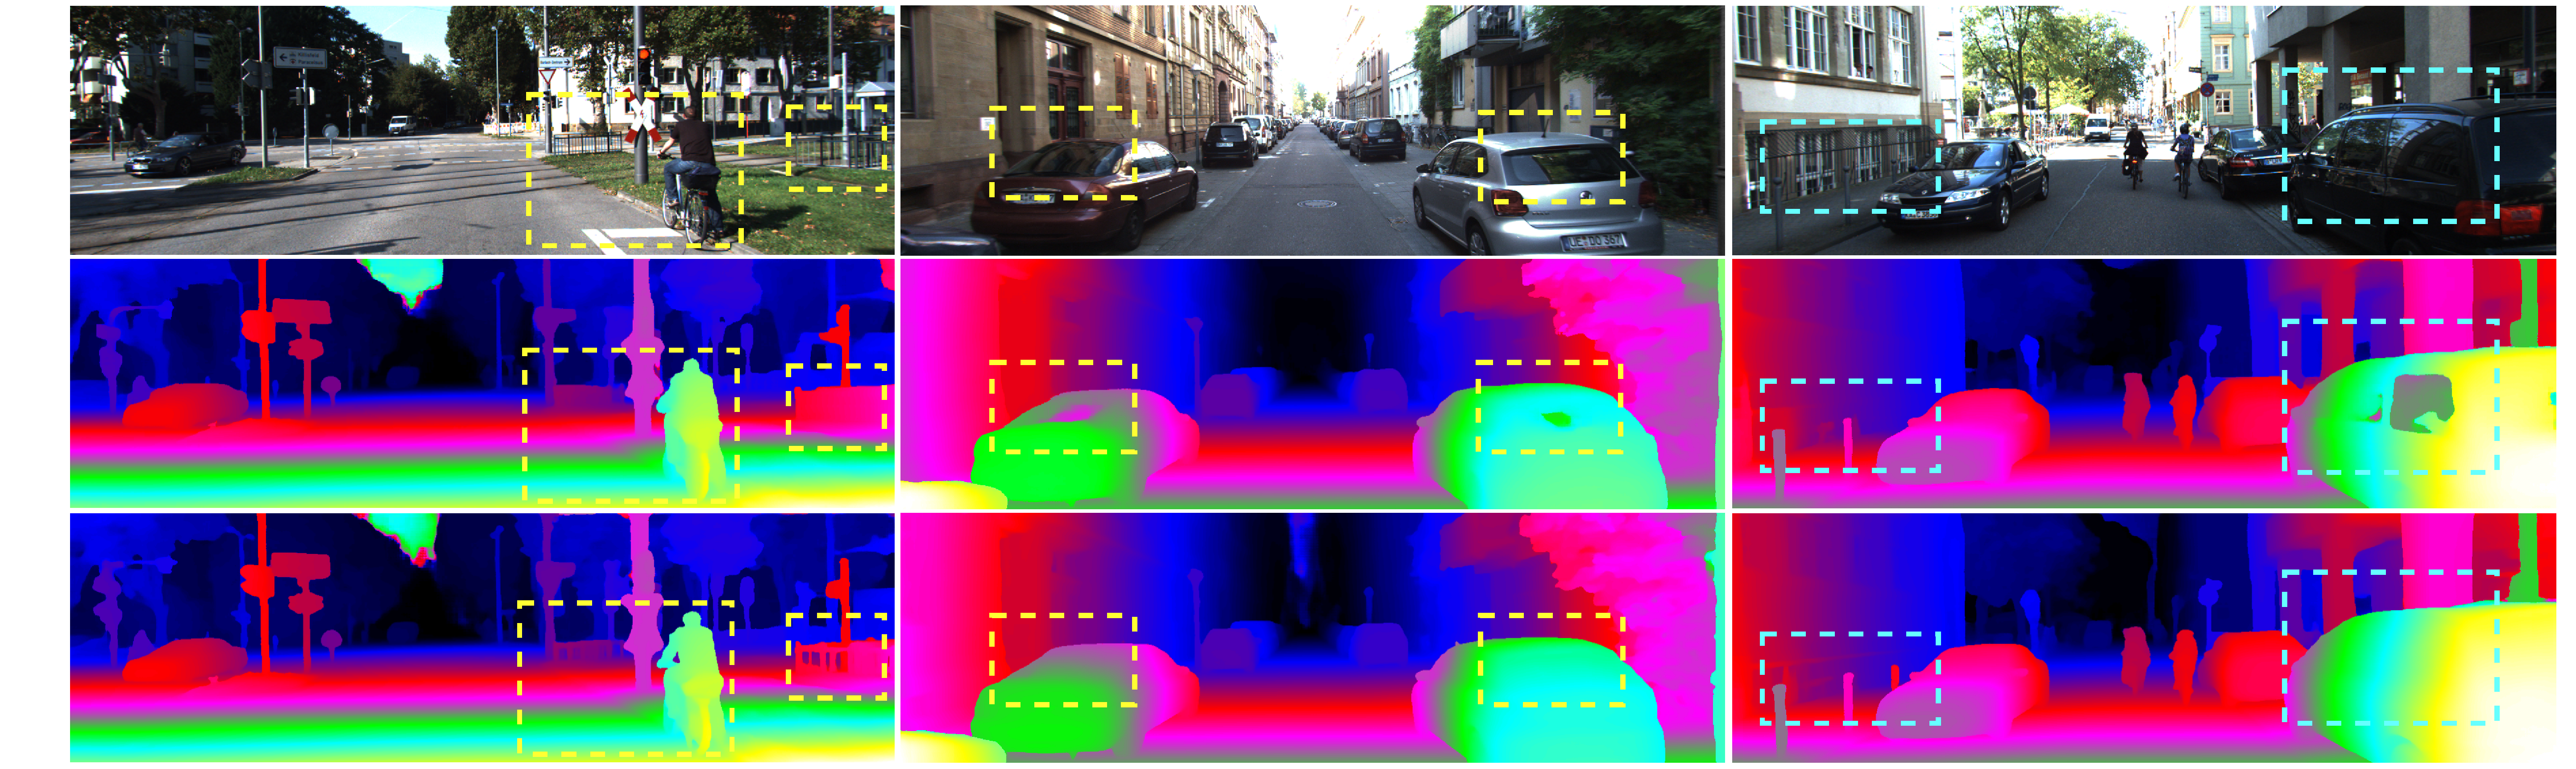
\includegraphics[width=0.96\linewidth]{fig/bridgedepth/kitti_ft.pdf} \\
	\end{tabular}
	\vspace{-0.5em}
	\caption{\textbf{Visual comparison on KITTI using a model fine-tuned on the combined KITTI 2012 and 2015 training sets}. 
	Relative to the state-of-the-art stereo method NMRF~\cite{guan2024neural}, the proposed approach better handles challenging regions such as transparent windows while maintaining fine structural detail.}
	\label{fig:kitti_ft}
	\vspace{-1.0em}
\end{figure}

\noindent\textbf{Zero-shot generalization.}
To evaluate cross-domain robustness, models trained only on Scene Flow are directly tested on real-world datasets without fine-tuning.
This setting is challenging for stereo matching because the appearance statistics, camera configurations, image noise, and disparity distributions differ significantly from the synthetic training domain.
The proposed stereo output improves substantially over the NMRF baseline on Middlebury and ETH3D.
The quantitative results are reported in Table~\ref{tab:bridge_zero_shot}. 
On Middlebury at quarter resolution, BP-2 error decreases from $7.5\%$ to $4.3\%$. On ETH3D, the BP-1 error decreases from $3.8\%$ to $1.3\%$.
The monocular output also generalizes well after alignment, indicating that stereo geometry improves the contextual branch rather than benefiting only the stereo prediction.
The substantial gains on ETH3D and Middlebury support the thesis argument that robust visual geometry benefits from combining complementary cues within a unified latent representation.

\begin{figure}[!t]
	\centering
	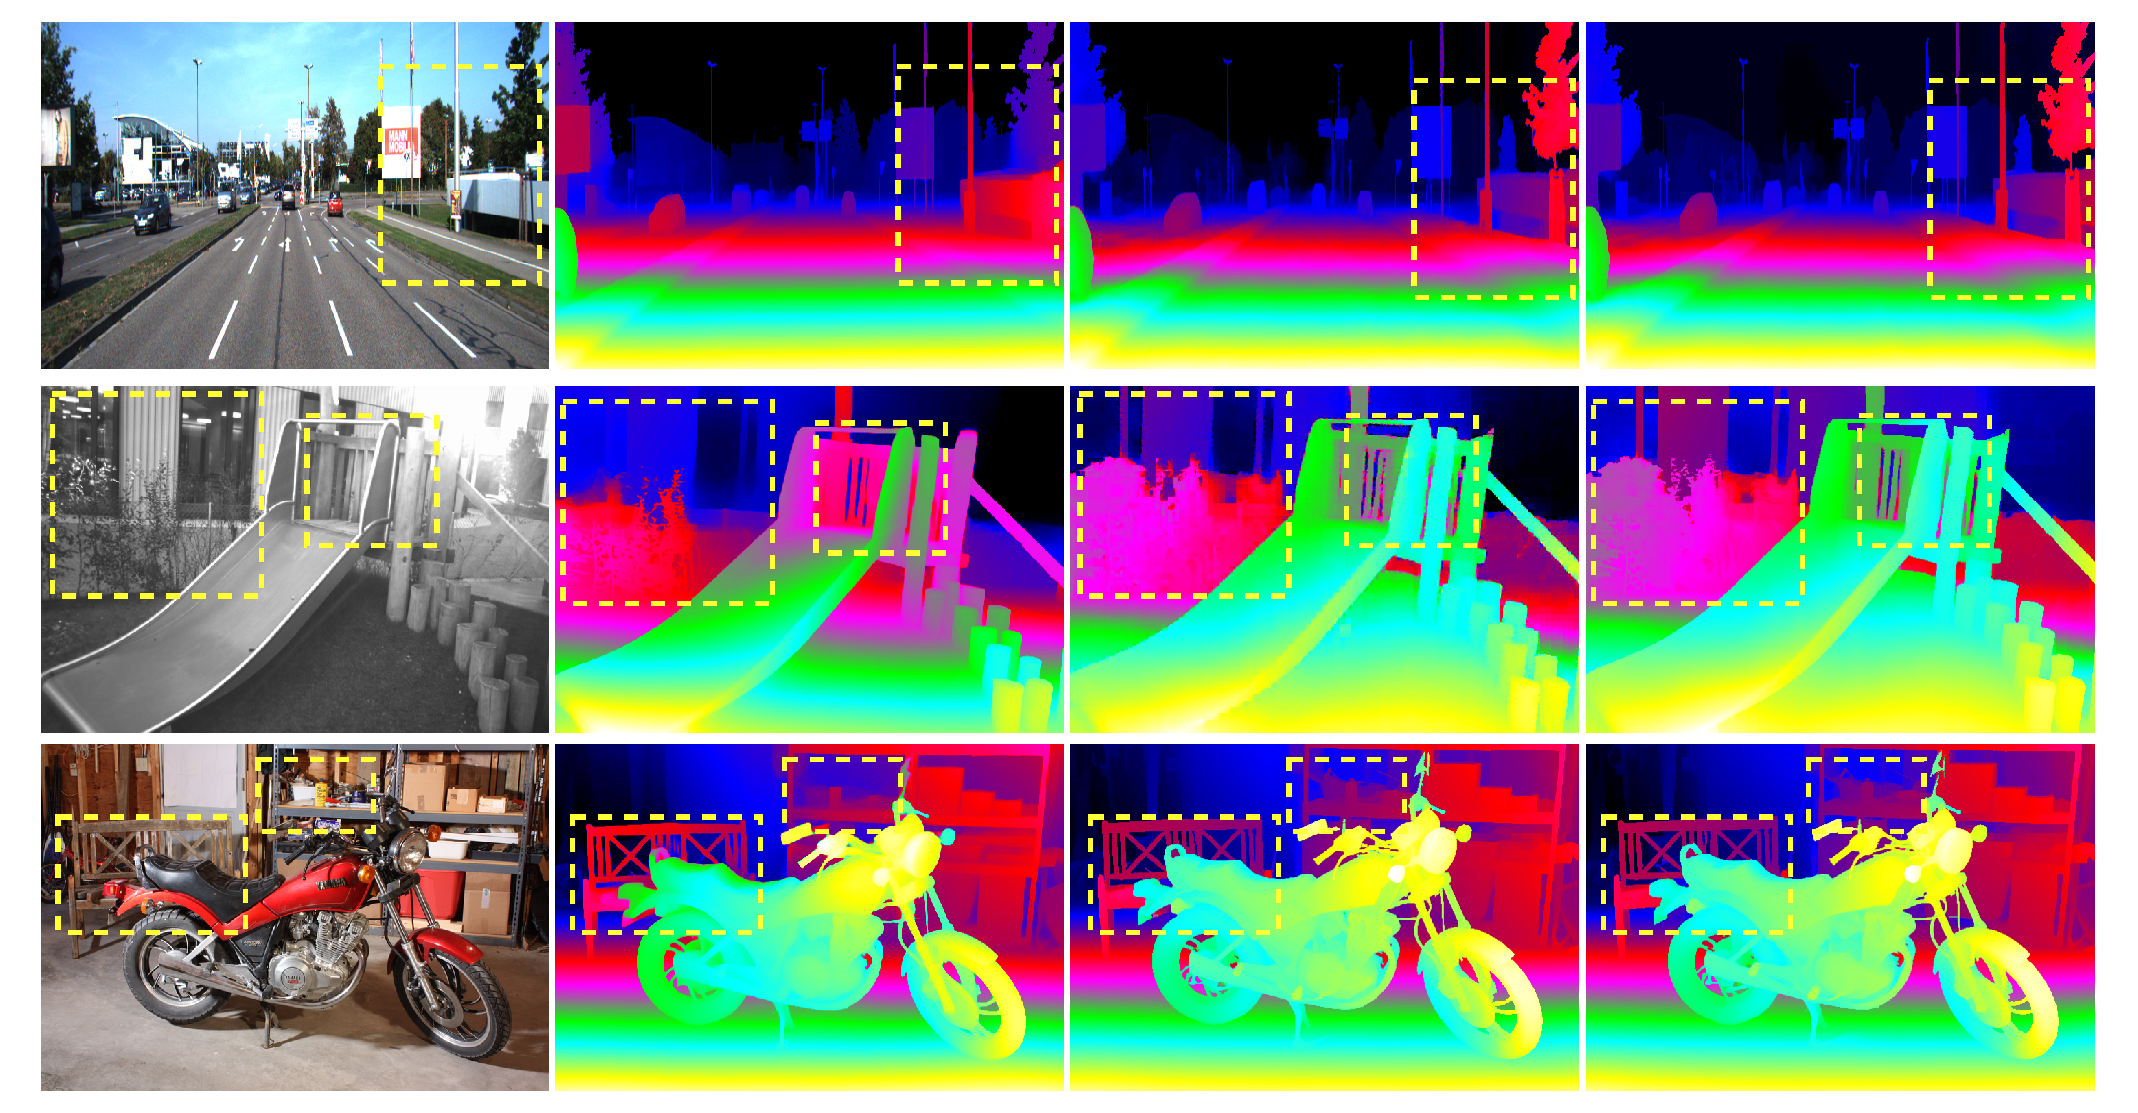
\includegraphics[width=1.0\linewidth]{fig/bridgedepth/zeroshot_mono.pdf}\\
	\vspace{-4pt}
	\makebox[0.245\linewidth]{\footnotesize\textsf{Input Image}}
	\makebox[0.24\linewidth]{\footnotesize\textsf{DAv2~\cite{yang2024depth}}}
	\makebox[0.24\linewidth]{\footnotesize\textsf{Ours-\emph{Mono}}}
	\makebox[0.245\linewidth]{\footnotesize\textsf{Ours-\emph{Stereo}}}\\
	\vspace{-4pt}
	\caption{\textbf{Zero-shot generalization of monocular depth outputs.} 
	Compared with DepthAnythingV2~\cite{yang2024depth}, the monocular stream of BridgeDepth produces estimates with stronger scale coherence and finer structural detail.}
	\label{fig:mono_zero}
	\vspace{-0.5em}
\end{figure}

\noindent\textbf{Ill-posed reflective and transparent regions.}
Qualitative evaluation on the Booster dataset, illustrated in Figure~\ref{fig:bridge_stereo_zero}, shows the benefit of latent alignment in regions where stereo correspondence is intrinsically ambiguous.
Matching-based stereo methods can produce fragmented predictions near mirrors, glass, transparent bottles, or specular hightlights because the apparent correspondence does not reliably represent the physical surface.
In contrast, the proposed method maintains more coherent surface structure by using monocular context to regularize stereo hypotheses.
This behavior is consistent with the design of the readout phase.
Stereo hypotheses query monocular features before aggregation, so the hypothesis representation has access to structural priors before selecting or propagating disparities.
As a result, the model is less likely to rely solely on local matching evidence in regions where that evidence is misleading.

\begin{figure}[!t]
	\centering
	\begin{minipage}{0.45\linewidth}
		\centering
		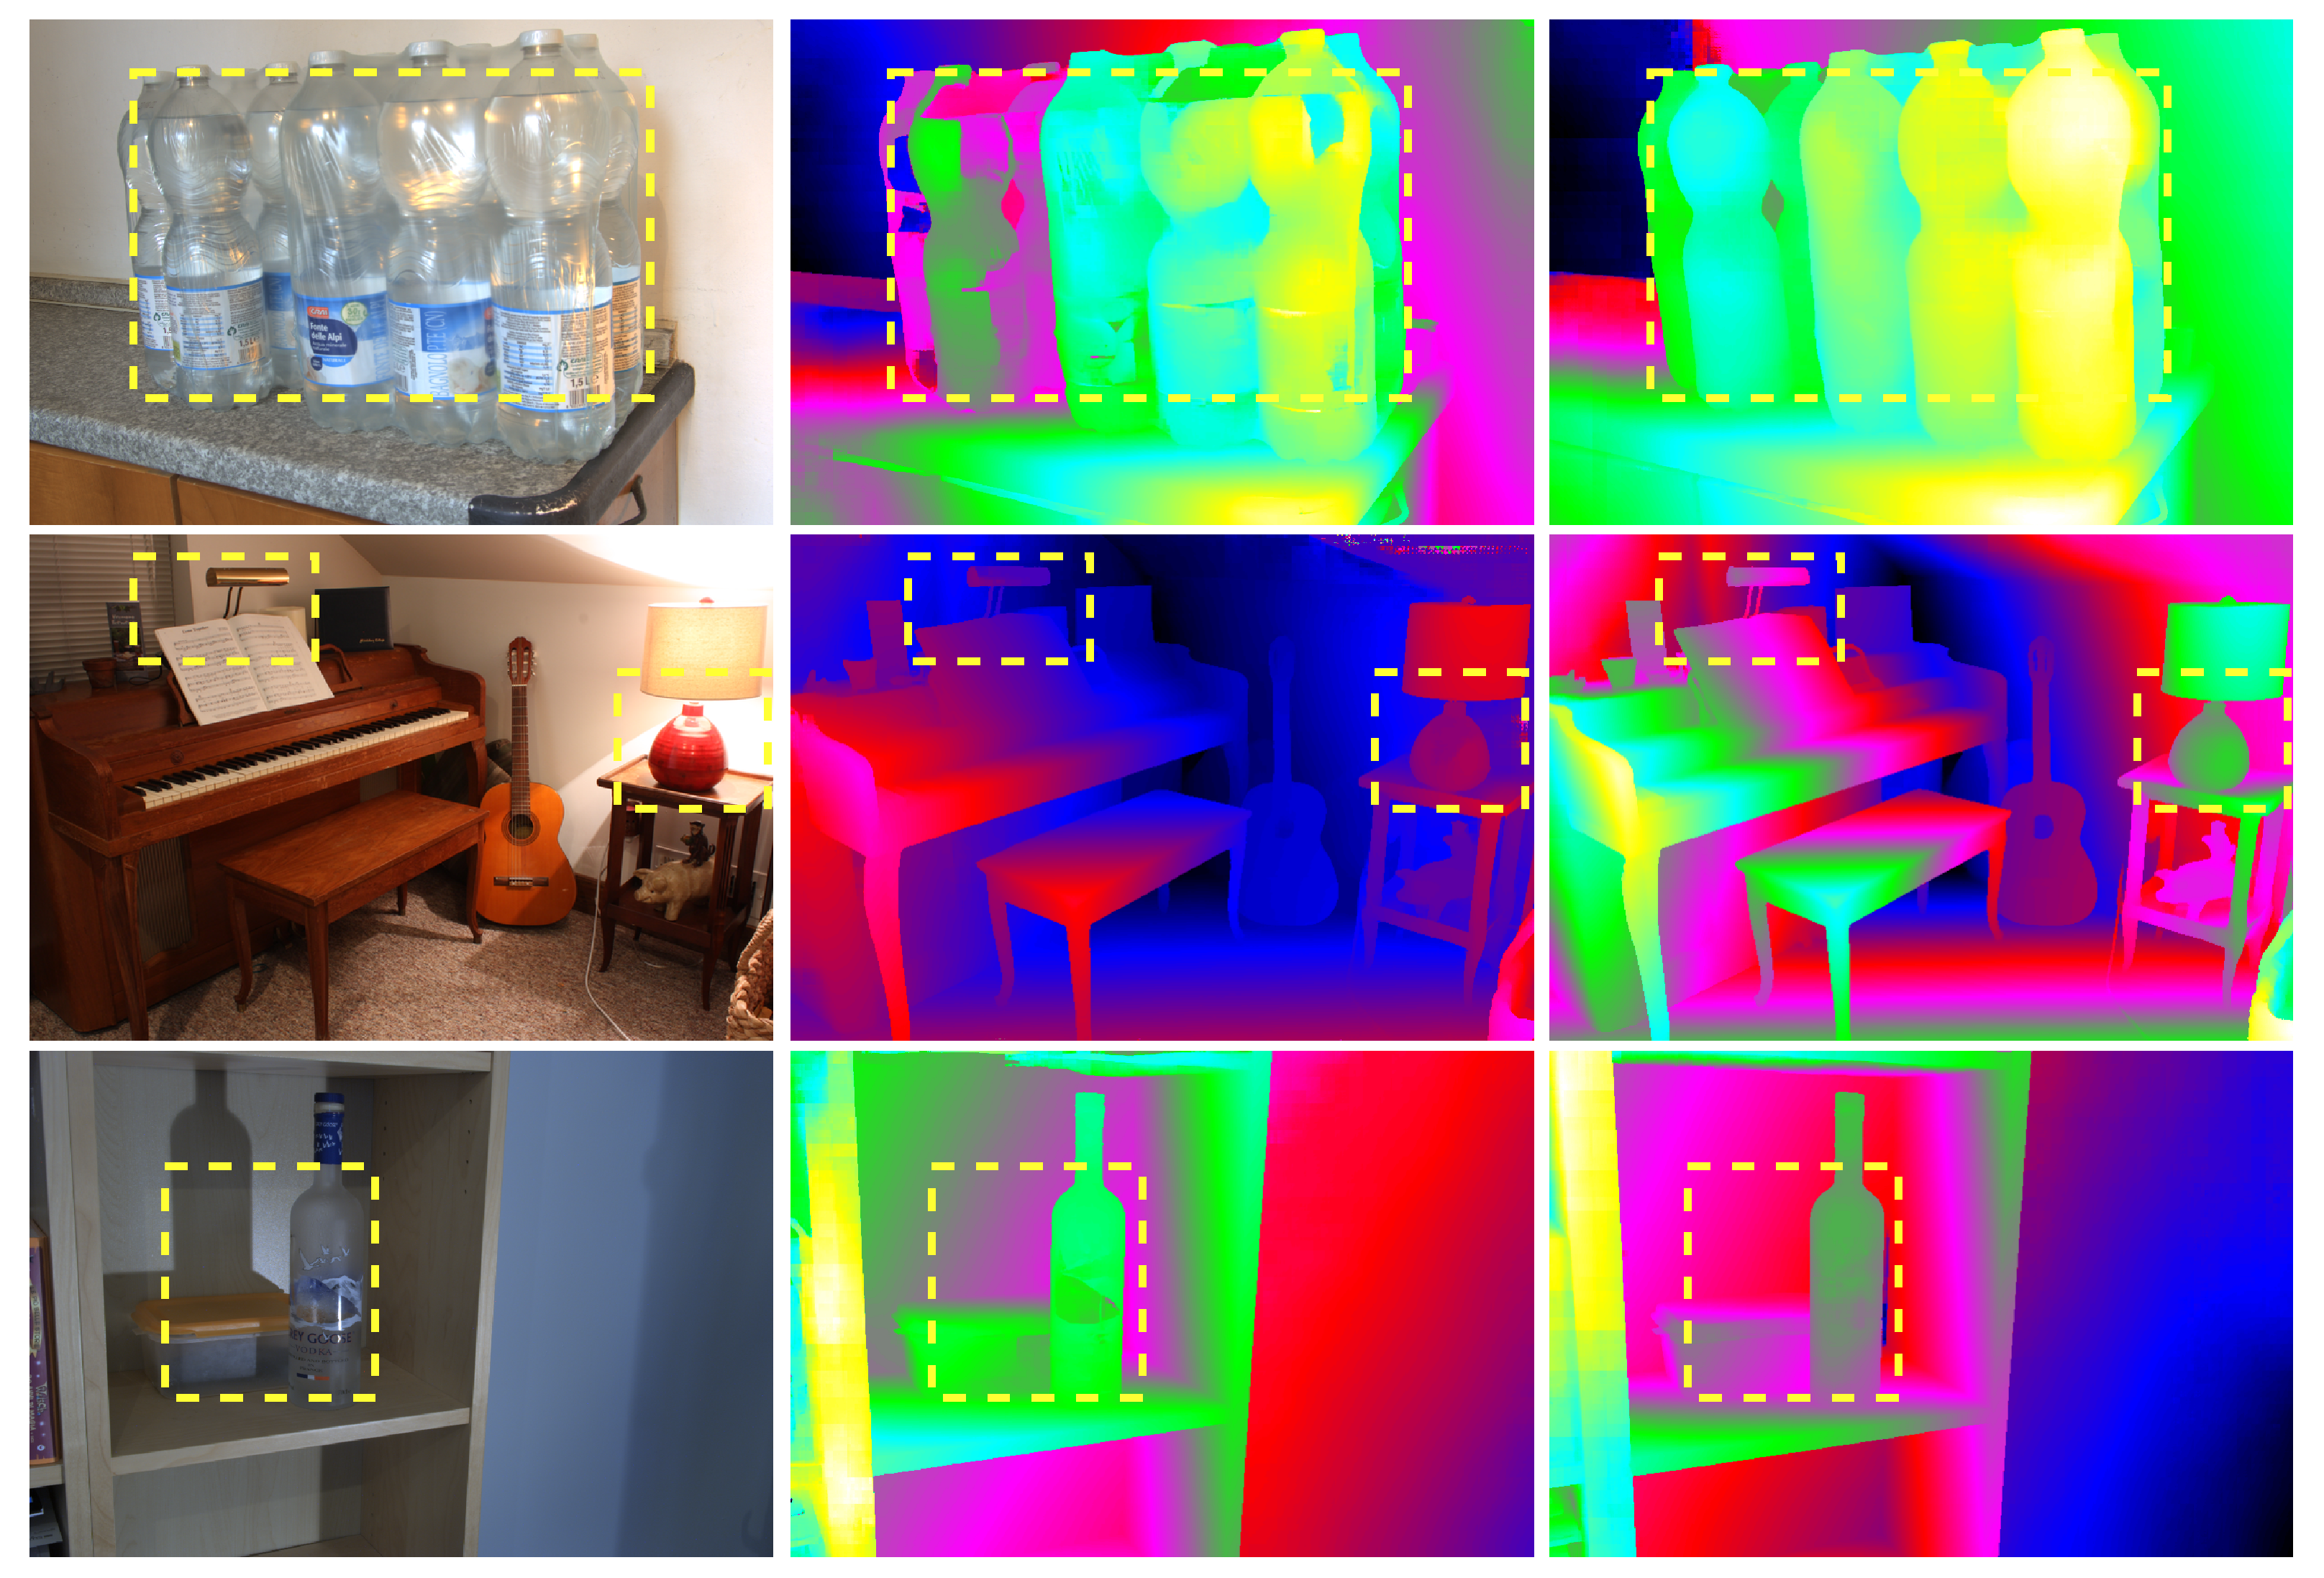
\includegraphics[width=\linewidth]{fig/bridgedepth/zero_stereo.pdf}
		\vspace{-3pt}
		\makebox[0.33\linewidth]{\footnotesize\textsf{Input Image}}
		\makebox[0.32\linewidth]{\footnotesize \textsf{NMRF}~\cite{guan2024neural}}
		\makebox[0.32\linewidth]{\footnotesize \textsf{Our-\emph{Stereo}}}
		%\subcaption{\textbf{Zero-shot stereo performance on ill-posed scenes.} Qualitative comparison between our method and the NMRF~\cite{guan2024neural} in difficult correspondence regions.}
		\captionof{figure}{\textbf{Zero-shot stereo performance on ill-posed scenes.}
		Qualitative comparison between the proposed method and NMRF~\cite{guan2024neural} in difficult correspondence regions.}
		\label{fig:bridge_stereo_zero}
	\end{minipage}
	\hfill
	\begin{minipage}{0.54\linewidth}
		\centering
		\resizebox{\linewidth}{!}{
		\begin{tabular}{l c c c c}
			\toprule
			\multirow{2}{*}{Methods} & KITTI-12 & KITTI-15 & Middlebury (Q) & ETH3D \\
			& (D1) & (D1) & (BP-2) & (BP-1) \\
			\midrule
			DSMNet~\cite{zhang2019domaininvariant} & 6.2 & 6.5 & 8.1 & 6.2\\
			Mask-CFNet~\cite{rao2023masked} & 4.8 & 5.8 & - & 5.7 \\
			
			CREStereo++~\cite{jing2023uncertainty} & 4.7 & 5.2 & - & 4.4\\
			Former-RAFT-DAM~\cite{zhang2024learning} & 3.9 & 5.1 & 5.4 & 3.3 \\
			RAFT-Stereo~\cite{lipson2021raft} & 4.7 & 5.5 & 9.4 & 3.3\\
			
			IGEV-Stereo~\cite{xu2023iterative} &5.2 & 5.7 & 8.8 & 4.0\\
			NMRF~\cite{guan2024neural} & 4.2 & 5.1 & 7.5 & 3.8\\
			IGEV++~\cite{xu2024igev++} & 5.1 & 5.9 & 7.8 & 4.1 \\
			FoundationStereo~\cite{wen2025foundationstereo} & \cellcolor{red!25}\textbf{3.2} & \cellcolor{yellow!25}4.9 & \cellcolor{yellow!25}5.5 & \cellcolor{yellow!25}1.8 \\
			\midrule
			BridgeDepth (Stereo) & \cellcolor{yellow!25}3.6 & \cellcolor{red!25}\textbf{4.5} & \cellcolor{red!25}\textbf{4.3} & \cellcolor{red!25}\textbf{1.3}\\
			BridgeDepth (Mono$^\dag$) & 3.7 & 4.2 & 5.8 & 1.7\\
			\bottomrule
		\end{tabular}
		}
		\captionof{table}{\textbf{Evaluation under zero-shot generalization.} All methods are trained exclusively on the Scene Flow dataset. The \colorbox{red!25}{\textbf{best}} and \colorbox{yellow!25}{second best} are color-coded. ($\dag$): Relative depth maps are aligned to ground truth using the ROE solver~\cite{wang2025moge}.}
		\label{tab:bridge_zero_shot}
	\end{minipage}
	%\vspace{-1.0em}
	%\caption{Left: Qualitative comparison on ill-posed stereo regions. Right: Quantitative zero-shot benchmarks for all methods trained solely on Scene Flow.}
\end{figure}

\noindent\textbf{ETH3D leaderboard evaluation.} On the ETH3D test set, the method also achieves state-of-the-art performance compared with recent stereo and hybrid systems.
As reported in Table~\ref{supp:tab_eth3d}, the method obtains $0.50\%$ BP-1 error, $0.16\%$ BP-2 error, $0.11$ pixel average error, and $0.26$ pixel RMS error.
These results demonstrate that our approach delivers accurate and robust depth estimation across diverse real-world conditions.

\begin{table}[!t]
	\centering
	\begin{subtable}{0.49\linewidth}
			%\vspace{0.2em}
			\footnotesize
			%\setlength\tabcolsep{2.5pt}
			%\renewcommand{\thetable}{{\alph{table}}}
			\centering
			\begin{tabular}{c|cccc}
				\toprule
				Method & BP-1 & BP-2 & AvgErr & RMS \\
				\midrule
				LoS~\cite{li2024local} & 1.03 & 0.32 & 0.15 & 0.34\\
				IGEV++~\cite{xu2024igev++} & 1.58 & 0.76 & 0.19 & 0.74\\
				Selective-IGEV~\cite{wang2024selective} & 1.56 & 0.51 & 0.15 & 0.57\\
				DEFOM-Stereo~\cite{jiang2025defom} & 0.78 & \underline{0.19} & \textbf{0.11} & \textbf{0.26}\\
				FoundationStereo~\cite{wen2025foundationstereo} & \textbf{0.48} & 0.26 & 0.13 & 0.61\\
				BridgeDepth (Ours) & \underline{0.50} & \textbf{0.16} & \textbf{0.11} & \textbf{0.26}\\
				\bottomrule
			\end{tabular}
			\caption{Performance on ETH3D test split}
			\label{supp:tab_eth3d}
	\end{subtable}
	\hfill
	\begin{subtable}{0.49\linewidth}
		\footnotesize
		\begin{tabular}{l c c c}
			\toprule
			& ETH3D & Middlebury & Time \\
			& (BP-1) & (BP-2) & (s) \\
			\midrule
			baseline (NMRF-s) & 3.7 & 8.0 & 0.044\\
			w/ monocular-readout & 2.3 & 5.9 & 0.123\\
			w/ monocular-update & 2.1 & 5.5 & 0.128\\
			w/ fine-grained & 1.6 & 4.8 & 0.147\\
			w/ monocular loss & 1.3 & 4.4 & 0.147\\
			\bottomrule
		\end{tabular}
		\caption{Impact assessment of individual architecture modules.}
		\label{tab:bridge_abl}
	\end{subtable}
	\vspace{-1.0em}
	\caption{Quantitative assessment of the proposed framework. Subtable (a) reports accuracy metrics on the ETH3D test set. Subtable (b) isolates the contribution of each architectural module through ablation.}
\end{table}

\noindent\textbf{Monocular output evaluation.} To evaluate the monocular stream, its relative depth prediction is aligned to the ground-truth disparity before computing the metrics.
Specifically, relative depth maps are aligned to ground truth using the ROE solver~\cite{wang2025moge}.
Compared with the original monocular foundation model and representative monocular metric depth models, the aligned monocular output achieves substantial improvement in Abs Rel and $\delta < 1.25$ across KITTI, ETH3D, and Middlebury, as shown in Table~\ref{supp:tab_depth}.
These results suggest that the monocular stream is not merely  a source of contextual priors for stereo matching.
Through bidirectional update, its latent representation is progressively grounded by aggregated stereo hypotheses and becomes more consistent with metric multi-view geometry.
This further verifies that BridgeDepth establishes mutual refinement between monocular context and stereo correspondence, rather than using monocular priors only as one-way guidance for stereo matching.

\begin{table}[t]
	%\vspace{-1em}
	\footnotesize
	\centering
	\begin{tabular}{c|cc|cc|cc|cc}
		\toprule
		\multirow{2}{*}{Model}& \multicolumn{2}{c|}{KITTI-12} & \multicolumn{2}{c|}{KITTI-15} & \multicolumn{2}{c|}{ETH3D} & \multicolumn{2}{c}{Middlebury}\\
		& Abs Rel $\downarrow$ & $\delta<1.25 \uparrow$ & Abs Rel $\downarrow$ & $\delta<1.25 \uparrow$ & Abs Rel $\downarrow$ & $\delta<1.25 \uparrow$ & Abs Rel $\downarrow$ & $\delta<1.25 \uparrow$ \\
		\midrule
		DAv2-L & 0.093 & 0.925 & 0.084 & 0.933 & 0.055 & 0.965 & 0.081 & 0.943\\
		UDv2-L & 0.054 & 0.967 & 0.067 & 0.949 & 0.052 & 0.972 & 0.056 & 0.982\\
		Ours & \textbf{0.033} & \textbf{0.982} & \textbf{0.048} & \textbf{0.975} & \textbf{0.020} & \textbf{1.000} & \textbf{0.019} & \textbf{0.990}\\
		\bottomrule
	\end{tabular}
	\vspace{-1.0em}
	\caption{\textbf{Monocular output evaluation.}
	Relative depth predictions are aligned to the ground-truth disparity using the ROE solver of MoGe~\cite{wang2025moge}.
	DAv2-L denotes the ViT-L variant of DepthAnythingV2, and UDv2-L denotes the ViT-L variant of UniDepthV2~\cite{piccinelli2025unidepthv2}.
	The monocular output of BridgeDepth achieves substantial improvement across KITTI, ETH3D, and Middlebury.
	}
	\label{supp:tab_depth}
	\vspace{-1.2em}
\end{table}

\subsection{Ablation Studies}
The ablation studies clarify how each component contributes to the central objective of this chapter: aligning monocular contextual reasoning with stereo hypothesis-based geometry.
Rather than treating the results only as incremental numeric improvements, the analysis focuses on three questions.
First, does the monocular stream provide useful structural priors for stereo matching under domain shift?
Second, does the reverse update from stereo to monocular representation contribute to genuine bidirectional alignment rather than one-way guidance?
Third, can the model recover fine geometric details without sacrificing the efficiency gained from compact stereo hypotheses?

All variants in Table~\ref{tab:bridge_abl} are trained only on Scene Flow and evaluated in the zero-shot setting on ETH3D and Middlebury.
This setting is intentionally chosen because it stresses the generalization ability of stereo matching.
A model trained only on synthetic data must handle real image statistics, different camera settings, grayscale imagery, and challenging regions where local correspondence evidence is often unreliable.
Improvement in this setting is therefore more informative than in-domain accuracy alone: it indicates whether the model has learned a more transferable form of geometric reasoning.
The baseline is a streamlined stereo-only model derived from NMRF~\cite{guan2024neural}.
It keeps the core hypothesis-based stereo formulation, including compact disparity proposals and neural message passing, but removes the monocular branch and all cross-modal alignment operations.
To make the comparison controlled and efficient, the baseline uses only two disparity hypotheses per pixel, matching the compact hypothesis representation used by BridgeDepth.
In this way, the baseline isolates the capability of stereo hypothesis reasoning alone.
Its performance reflects the limitation of relying only on binocular evidence when the candidate disparity set is small and the test domain differs from the training domain.

\noindent\textbf{Monocular readout.} As shown in Table~\ref{tab:bridge_abl}, adding monocular readout brings the most significant improvement.
In this variant, stereo hypotheses query monocular contextual representations before neural message passing.
This result confirms the primary motivation of this chapter: monocular representations are more useful when they participate in stereo reasoning before the model aggregates and selects hypotheses.
Since readout is applied before cost aggregation, contextual cues about scene layout, object structure, and surface continuity can guide how ambiguous hypotheses are propagated and suppressed.
The substantial improvement on ETH3D, where BP-1 decreases from 3.7\% to 2.3\%, and on Middlebury, where BP-2 decreases from 8.0\% to 5.9\%, suggests that monocular priors help compensate for unreliable correspondence evidence under domain shift.

\noindent\textbf{Monocular update.} The monocular update module completes the bidirectional alignment loop. 
Compared with monocular readout alone, the gain in stereo metrics is moderate, which is expected because the update primarily refines the monocular representation rather than directly changing the current stereo hypotheses.
Its value lies in the iterative nature of the model: once the monocular stream has absorbed aggregated stereo evidence, the updated contextual representation can provide more geometry-aware guidance in subsequent alignment blocks.
Therefore, the update step should not be interpreted only by its immediate numeric improvement in the stereo output.
It is important because it changes the role of the monocular stream from a fixed source of priors into a geometry-grounded representation that participates in mutual refinement.

\noindent\textbf{Fine-grained refinement.} The fine-grained refinement stage addresses a different limitation of the coarse alignment process.
The main bidirectional alignment operates at $1/8$ resolution for efficiency, which is suitable for robust global reasoning but insufficient for thin structures, sharp boundaries, and small disparity variations.
The fine stage initializes high-resolution stereo embeddings from the coarse prediction and performs additional alignment at $1/4$ resolution.
Importantly, the monocular stream remains at the coarse resolution, and the interaction window is adjusted to preserve a comparable receptive field.
This asymmetric design improves detail recovery while avoiding the high computational cost of full high-resolution cross-modal alignment.
The ablation therefore shows that fine-scale stereo evidence and coarse contextual priors can be combined efficiently.

\noindent\textbf{Monocular loss.} Finally, adding the monocular loss produces the strongest generalization performance.
This loss does not merely provide auxiliary supervision to an additional output.
It explicitly encourages the monocular representation to remain consistent with ground-truth geometry after receiving stereo updates.
As a result, bidirectional alignment is strengthened from both directions: stereo hypotheses are guided by monocular context, and monocular representations are encouraged to encode geometry consistent with stereo disparity.
The qualitative comparison in Figure~\ref{fig:abl} further supports this interpretation, showing that monocular supervision improves the structural consistency of the aligned representation and reduce artifacts in ambiguous regions.

\begin{figure}[!t]
	\centering
	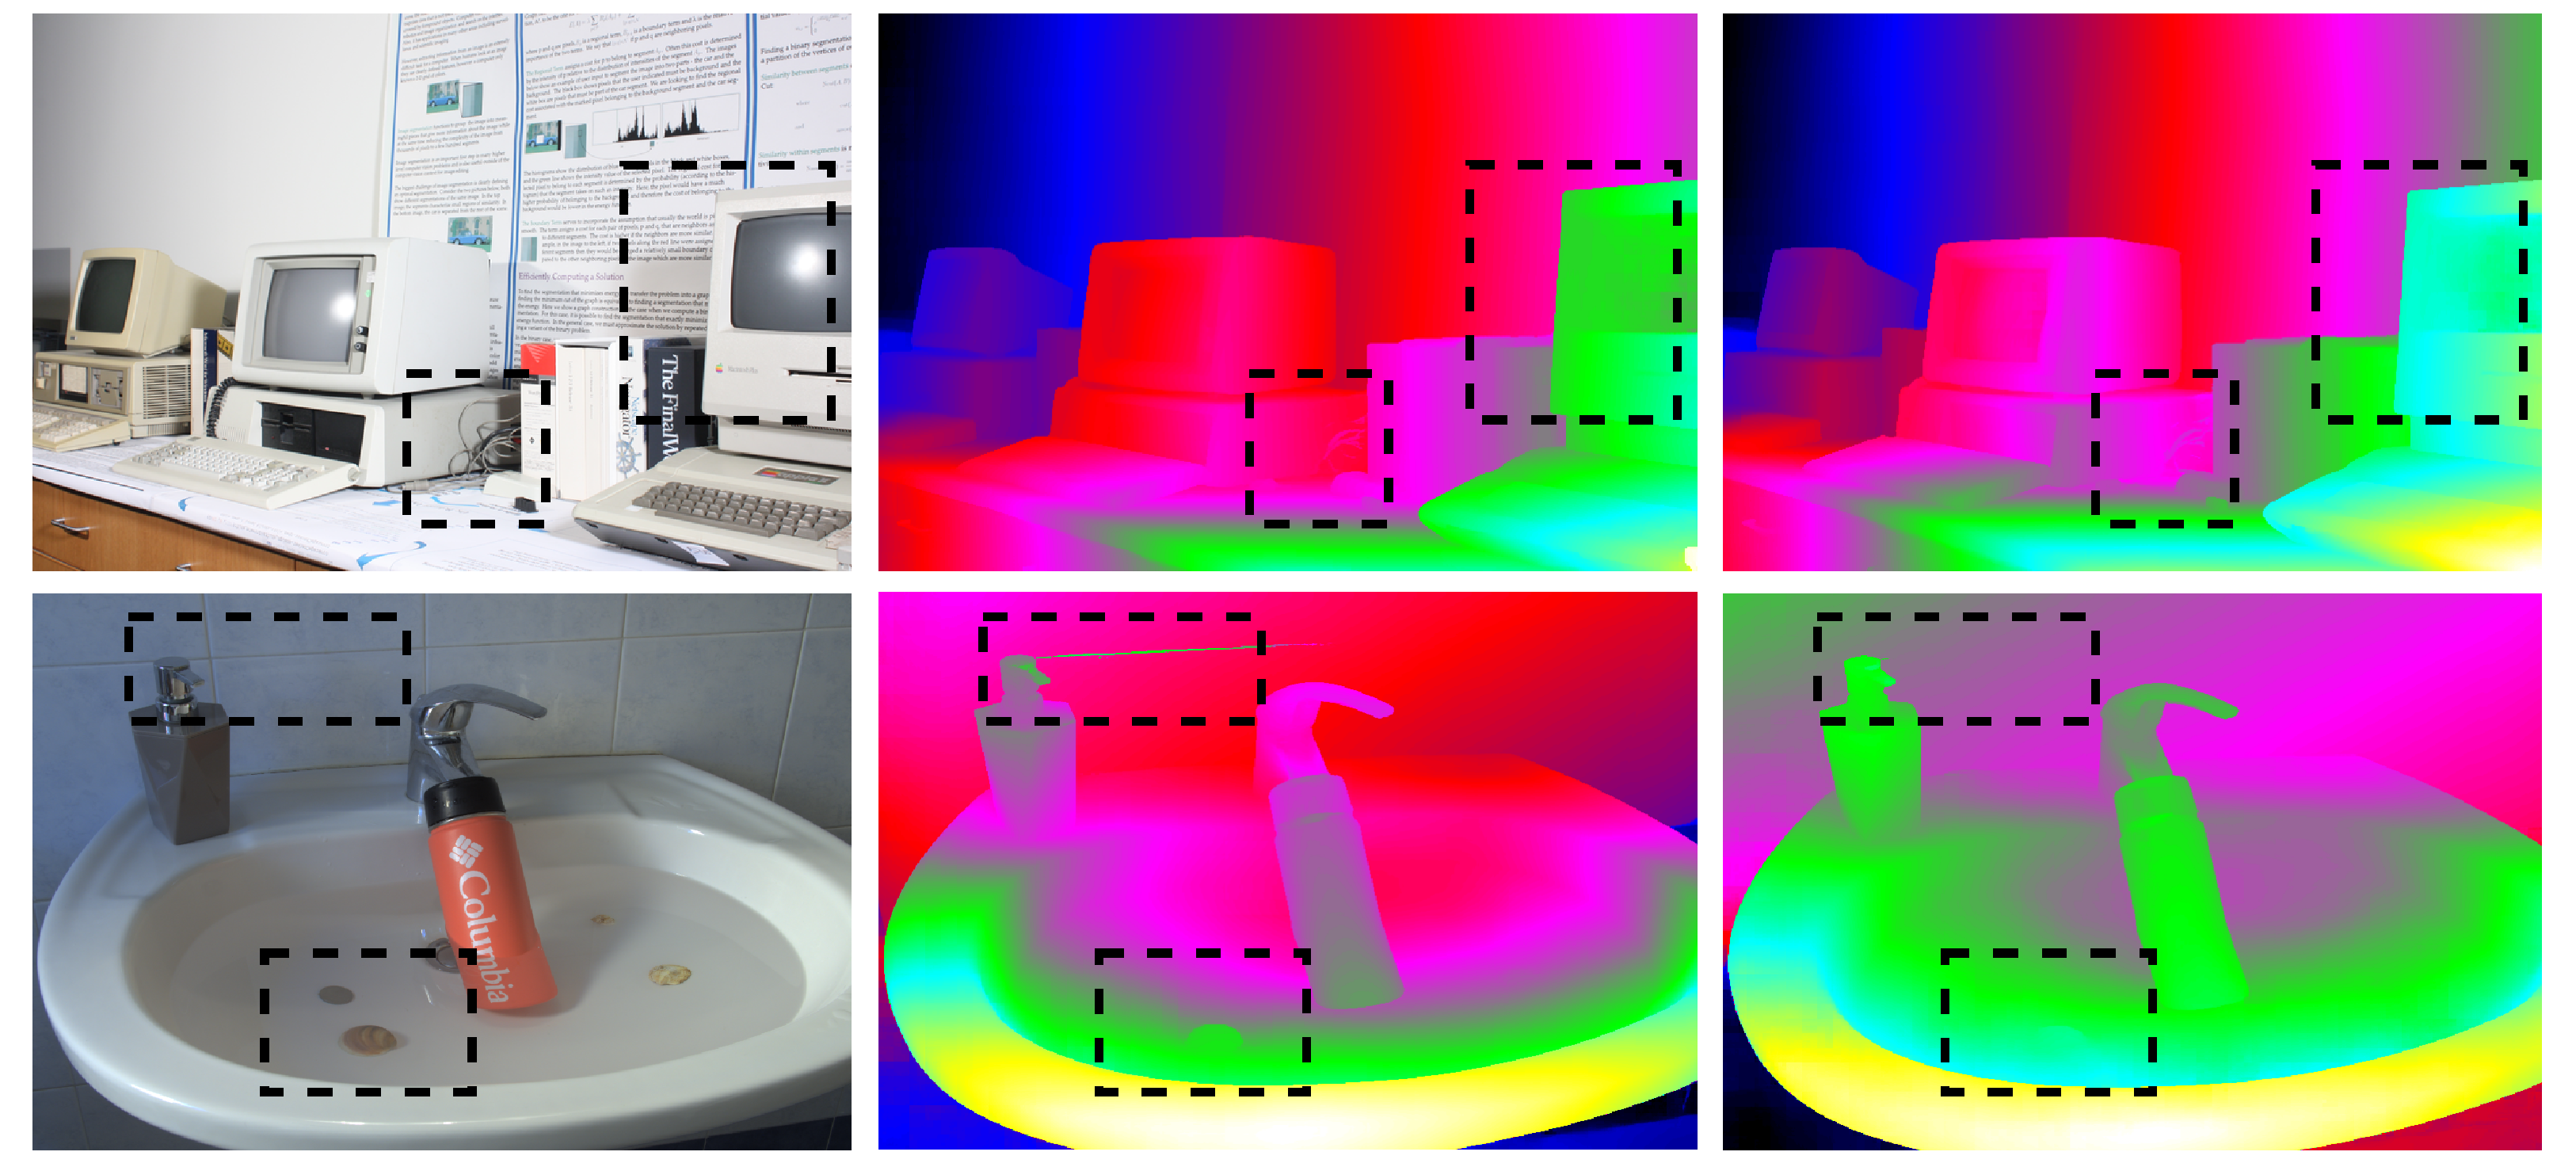
\includegraphics[width=0.75\linewidth]{fig/bridgedepth/abl.pdf}\\
		\vspace{-4pt}
		\makebox[0.25\linewidth]{\footnotesize\textsf{Input Image}}
		\makebox[0.24\linewidth]{\footnotesize $\mathcal{L}_{\text{stereo}}$}
		\makebox[0.25\linewidth]{\footnotesize$\mathcal{L}_{\text{stereo}}+\mathcal{L}_{\text{mono}}$}\\
		%\includegraphics[width=0.97\linewidth]{figs/zero-shot-booster.pdf}
		\vspace{-0.3em}
		\captionof{figure}{\textbf{Effect of monocular supervision.}
		Adding the monocular loss improves the geometric consistency of the aligned representation, producing more coherent depth structures in ambiguous regions than stereo-only supervision.}
		\label{fig:abl}
\end{figure}

\begin{table}[!t]
	\centering
	\footnotesize
	\begin{tabular}{c|c|cccc}
		\toprule
		\multirow{2}{*}{Backbone} & SceneFlow & KITTI-12 & KITTI-15 & ETH3D & Middlebury (Q)\\
		& EPE $\downarrow$ & D1 $\downarrow$ & D1 $\downarrow$ & BP-1 $\downarrow$ & BP-2 $\downarrow$\\
		\midrule
		baseline & 0.47 & 4.5 & 5.2 & 3.7 & 8.0\\
		\rowcolor{lightgray}
		DAv2-B & 0.37 & 3.8 & 4.7 & 1.4 & 4.7\\
		DAv2-L & 0.37 & 3.7 & 4.5 & 1.3 & 4.4\\
		UDv2 & 0.36 & 3.7 & 4.8 & 1.8 & 5.1\\
		MoGe & 0.36 & 3.3 & 4.5 & 1.8 & 5.1\\
		\midrule
		\rowcolor{lightgray}
		DAv2-B (post-hoc)&0.44&4.1&4.8&3.2&7.4\\
		\bottomrule
	\end{tabular}
	\vspace{-0.3em}
	\captionof{table}{\textbf{Ablation of monocular foundation models and fusion strategy.}
	We report in-domain accuracy on Scene Flow and zero-shot generalization on real-world datasets.
	The baseline is the NMRF model used in Table~\ref{tab:bridge_abl}.
	Here, DAv2 denotes DepthAnythingV2, and UDv2 denotes UniDepthV2.
	The gray rows use the same DAv2-B backbone to compare latent alignment with post-hoc fusion, showing that interaction during hypothesis reasoning is more effective than late-stage fusion.
	}
	\label{tab:mono_foundation}
	\vspace{-1.0em}
\end{table}

\noindent\textbf{Monocular foundation models and post-hoc fusion.} 
Beyond the main component analysis in Table~\ref{tab:bridge_abl}, additional ablations examine whether the proposed mechanism depends on a particular monocular foundation model and whether iterative alignment is preferable to post-hoc fusion. 
Replacing the monocular backbone with different foundation models still yields clear improvements over the stereo-only baseline, as shown in Table~\ref{tab:mono_foundation}).
This indicates that the framework is not tied to one specific monocular architecture.
Although the backbone affects final accuracy to some extent, the consistent trend suggests that the benefit comes from the alignment mechanism itself: stereo hypotheses can exploit high-level monocular structure as long as the monocular branch provides meaningful contextual features.

The post-hoc fusion ablation further clarifies this point.
In that variant, monocular features are fused with the already aggregated stereo representation using a lightweight residual network, bypassing the iterative readout-update process.
Although this static fusion introduces additional monocular context, it performs noticeably worse than bidirectional latent alignment, as shown in Table~\ref{tab:mono_foundation}).
This comparison is important for the thesis argument.
It shows that the gain does not simply come from adding a monocular stream or increasing model capacity.
The crucial factor is when and how the modalities interact.
If the modalities are fused only after most reasoning has already been completed, monocular context cannot effectively guide hypothesis selection, and stereo geometry cannot progressively ground the monocular representation.
Dynamic alignment during inference is therefore essential for learning a unified geometric representation.

Overall, the ablation studies support the design principle of BridgeDepth.
The stereo-only baseline demonstrates the limitation of matching-centric reasoning in ambiguous regions.
Monocular readout shows that contextual priors are most effective when introduced before stereo aggregation.
Monocular update and monocular supervision demonstrate that the monocular stream can be made geometry-aware rather than remaining a fixed prior.
Fine-grained refinement shows that local detail can be recovered without abandoning the efficient coarse alignment design.
Together, these results validate the central claim of this chapter: robust depth estimation benefits from a shared latent space in which monocular context and stereo correspondence are repeatedly exchanged and refined.

\section{Discussion}
\subsection{Why Latent Alignment Improves Generalization}
The improvement in zero-shot generalization can be understood from the different failure modes of monocular and stereo estimation.
Stereo matching depends on local correspondence evidence and therefore suffers when the target domain changes appearance statistics or contains ambiguous surfaces.
Monocular foundation models, trained on diverse data, encode more domain-robust priors about object shape and scene layout.
By allowing stereo hypotheses to read from monocular features during aggregation, the model can use these priors to regularize matching in unfamiliar domains.
At the same time, monocular prediction lacks metric grounding.
The update operation addresses this limitation by injecting aggregated stereo evidence into the monocular stream.
The resulting monocular representation is not merely a prior learned from single images; it becomes conditioned on multi-view geometry.
This mutual refinement explains why both outputs improve.

\subsection{Relation to the Thesis Narrative}
This chapter fits into the broader thesis theme of learning visual geometry by unifying complementary cues.
Stereo correspondence provides spatial geometry through multi-view constraints, while monocular depth estimation provides semantic and structural priors.
Neither cue is sufficient in isolation.
Stereo is precise but fragile under ambiguity; monocular reasoning is robust but geometrically under-constrained.
The latent alignment framework shows how a neural network can explicitly coordinate these cues in representation space.
The same principle extends naturally to temporal geometry.
Optical flow and camera motion provide another source of geometric information, but they also suffer from ambiguity, occlusion, and appearance changes.
A future geometry-native architecture could similarly align temporal correspondence representation with monocular structural priors.
Thus, the contribution of this chapter is not only a stereo depth estimator, but also a concrete example of the thesis hypothesis: robust depth and motion perception requires unified representations that allow different geometric cues to interact during inference.

\subsection{Limitations}
Although the proposed framework improves robustness and generalization, it still has limitations.
First, the use of a top-$K$ disparity proposal module may become restrictive at very high image resolutions or under very large disparity ranges.
If the correct disparity is not retained among the selected candidates, later alignment cannot recover it.
This issue can become more pronounced for images above 2K or scenes with a large disparity range.
Second, the monocular stream introduces additional computation and memory compared with a purely stereo network.
Although the proposed approach remains highly efficient relative to many concurrent hybrid systems, the cost of using a large monocular foundation model is non-negligible.

\section{Conclusion}
This chapter presented a latent alignment framework for bridging monocular contextual reasoning and stereo geometric matching.
The proposed model represents stereo matching as a compact set of disparity hypotheses and aligns these hypotheses with monocular foundation representations through iterative bidirectional cross-attention.
Monocular readout injects semantic and structural priors into stereo aggregation, while monocular update feeds geometrically validated stereo evidence back into the contextual representation. 
A coarse-to-fine refinement stage recovers local details, and a dual-output training objective jointly supervises metric disparity and relative depth.
Extensive experiments demonstrate that the framework improves both in-domain stereo accuracy and zero-shot generalization. 
It is especially effective in challenging regions where pure stereo matching is unreliable, such as reflective and transparent surfaces. 
Ablation studies confirm that dynamic latent alignment outperforms post-hoc fusion and that dual loss strengthens cross-modal consistency.

Within the thesis, this chapter provides an important step toward unified visual geometry learning.
It shows that monocular priors and stereo correspondences should not be treated as isolated modules, but as complementary cues that can be aligned and refined within a shared latent space.
This principle motivates the broader pursuit of depth and motion perception systems that integrate spatial, semantic, and temporal geometry in a coherent learning framework.

\chapter{Chapter 5}

\chapter{...}



%%%%%%%%%%%%%%%% BACK MATTER %%%%%%%%%%%%%%%%

% Put appendices, bibliography, and supplemental materials here

% The bibliography may be single spaced within each entry, but must be
% double-spaced between each entry. Most bibliography styles leave space between
% entries, so that shouldn't be a problem.
\begin{singlespacing}
  % I like "References" better than "Bibliography"
  \renewcommand{\bibname}{References}

  % Any bibliohgraphy style that leaves space between entries is fine
  %\bibliographystyle{acl_natbib}
  %\bibliographystyle{ieeenat_fullname}
  \bibliographystyle{plain}
  %\bibliographystyle{ecca}
  \bibliography{references}
\end{singlespacing}

% Appendices from all chapters should go at the end
%\input{appendix}

\end{document}
